\documentclass[11pt, a4paper, norsk]{NTNUlf}
\usepackage[utf8]{inputenc}
\usepackage[T1]{fontenc}
\usepackage{float}
\usepackage{graphicx}
\usepackage{enumitem}
\usepackage{pdfpages}
\usepackage{amsthm}
\usepackage{pgfplots}
\pgfplotsset{compat=1.15}
\usepackage{mathrsfs}
\usetikzlibrary{arrows}
\usepackage{cleveref}

\setlength{\intextsep}{2.0pt plus 2.0pt minus 4.0pt}
%\setlength{\abovecaptionskip}{-15pt}

\newcommand{\R}{\mathbb{R}}

\newtheorem{lemma}{Lemma}
 
\ovingnr{7}
\semester{Vår 2022}
\fag{MA2401 Geometri}
\institutt{Institutt for matematiske fag}
 
\begin{document}

%
 
\begin{oppgave}[1.6.3]
  Først observerer vi at det skraverte området i figuren til venstre er et kvadrat,
  siden summen av de to spisse vinklene i trekanten $\triangle ABC$ er $90^\circ$. 
  Vi ønsker å vise at det skraverte området i figuren til venstre (med areal $c^2$) 
  er like stort som det skraverte område i figuren til høyre (med areal $a^2+b^2$). 
  Begge de to store ytre kvadratene er like store, da sidene er $a+b$. Begge figurene
  inneholder fire kopier av trekanten $\triangle ABC$ (altså de hvite områdene i
  figurene). Dermed (ved å trekke fra disse fire trekantene) må de skraverte områdene
  i begge figurene være like store, altså har vi $a^2+b^2 = c^2$. 
\end{oppgave}
 
\begin{oppgave}[1.6.6]
  Merk at det er mange måter å løse disse oppgavene på, kun en av de er beskrevet her. 
  \begin{punkt}
    Konstruer to sirkler: den første skal skjære $B$ og ha sentrum i $A$; den andre 
    skal skjære $A$ og ha sentrum i $B$. Disse sirklene skjærer hverandre i to punkter. 
    Tegn en linje mellom disse to punktene. Dette er linjen vi er ute etter, altså 
    midtnormalen til linjen $\overline{AB}$. 
    \begin{figure}[H]
      \centering
      
\definecolor{qqqqff}{rgb}{0,0,1}
\begin{tikzpicture}[line cap=round,line join=round,>=triangle 45,x=1cm,y=1cm]
\clip(-4,-3.5) rectangle (7,3.5);
\draw [line width=1.2pt,domain=-7.428317161275942:7.849176681756118] plot(\x,{(-0-0*\x)/3});
\draw [line width=1.2pt] (0,0) circle (3cm);
\draw [line width=1.2pt] (3,0) circle (3cm);
\draw [line width=1.2pt] (1.5,-4.570805445724599) -- (1.5,4.135407391746856);
\begin{scriptsize}
\draw [fill=qqqqff] (0,0) circle (2pt);
\draw[color=qqqqff] (0.1831173115481543,0.1936181149389139) node {$A$};
\draw [fill=qqqqff] (3,0) circle (2.5pt);
\draw[color=qqqqff] (3.179856488450597,0.21320464550690366) node {$B$};
\end{scriptsize}
\end{tikzpicture}

      \caption{Midtnormalen til $\overline{AB}$}
    \end{figure}
  \end{punkt}

  \begin{punkt}
    Lag en sirkel med sentrum i punktet $P$ slik at sirkelen skjærer linjen $l$ i to 
    punkter -- kall disse $A$ og $B$. Konstruer midtnormalen til linjestykket 
    $\overline{AB}$, slik som i oppgave a). Denne linjen vil ved konstruksjon være 
    normal på $l$ og skjære $P$. 
    \begin{figure}[H]
      \centering
      

\definecolor{qqqqff}{rgb}{0,0,1}
\begin{tikzpicture}[line cap=round,line join=round,>=triangle 45,x=1cm,y=1cm]
\clip(-4,-3.5) rectangle (7,4);
\draw [line width=1.2pt,domain=-7.428317161275942:7.849176681756118] plot(\x,{(-0-0*\x)/3});
\draw [line width=1.2pt] (0,0) circle (3cm);
\draw [line width=1.2pt] (3,0) circle (3cm);
\draw [line width=1.2pt] (1.5,-4.443492997032665) -- (1.5,4.262719840438789);
\draw [line width=1.2pt] (1.5,1.393016028085612) circle (2.047069528497607cm);
\begin{scriptsize}
\draw [fill=qqqqff] (0,0) circle (2pt);
\draw[color=qqqqff] (0.1831173115481543,0.2436181149389139) node {$A$};
\draw [fill=qqqqff] (3,0) circle (2.5pt);
\draw[color=qqqqff] (2.779856488450597,0.21320464550690366) node {$B$};
\draw [fill=qqqqff] (1.5,3.440085556583219) circle (2.5pt);
\draw[color=qqqqff] (1.6814868999993756,3.750640760189109) node {$C$};
\end{scriptsize}
\end{tikzpicture}

    \end{figure}
  \end{punkt}

  \begin{punkt}
    Lag en sirkel med sentrum i $A$. Denne sirkelen skjærer linjestykkene $\overline{AB}$ 
    og $\overline{BC}$ i to punkter, kall disse $D$ og $E$ respektivt. Konstruer 
    midtnormalen til linjestykket $\overline{DE}$, denne linjen vil være 
    vinkelhalveringsstrålen til $\angle BAC$.
    
    \begin{figure}[H]
      \centering
      
\definecolor{qqqqff}{rgb}{0,0,1}
\begin{tikzpicture}[line cap=round,line join=round,>=triangle 45,x=1cm,y=1cm]
\clip(-4,-3.5) rectangle (7,3.5);
\draw [line width=1.2pt] (0,0)-- (5,2);
\draw [line width=1.2pt] (0,0)-- (5,-1);
\draw [line width=1.2pt] (0,0) circle (3.2310988842807022cm);
\draw [line width=1.2pt] (3,1.2) circle (1.841382833093036cm);
\draw [line width=1.2pt] (3.1683531271721495,-0.6336706254344299) circle (1.841382833093036cm);
\draw [line width=1.2pt,domain=-9.298830830518968:9.504238514751254] plot(\x,{(-0--0.16835312717214945*\x)/1.8336706254344297});
\begin{scriptsize}
\draw [fill=qqqqff] (0,0) circle (2.5pt);
\draw[color=qqqqff] (-0.17150758583571446,0.26217097192687866) node {A};
\draw [fill=qqqqff] (5,2) circle (2.5pt);
\draw[color=qqqqff] (5.253961381497465,2.1228913758859074) node {B};
\draw [fill=qqqqff] (5,-1) circle (2.5pt);
\draw[color=qqqqff] (5.253961381497465,-1.0599198414124311) node {C};
\draw [fill=qqqqff] (3,1.2) circle (2.5pt);
\draw[color=qqqqff] (3.079856488450595,1.4863291324262398) node {D};
\draw [fill=qqqqff] (3.1683531271721495,-0.6336706254344299) circle (2pt);
\draw[color=qqqqff] (3.3267554677105186,-0.905294944028564) node {E};
\end{scriptsize}
\end{tikzpicture}

      \caption{Vinkelhalveringsstrålen til $\angle BAC$}
    \end{figure}
  \end{punkt}
\end{oppgave}

\begin{oppgave}[1.6.7]

  \begin{punkt}
    Nei. Euklids postulater sier oss ingen ting om antall punkter på linjer. 
  \end{punkt}

  \begin{punkt}
    Nei. Euklids postulater sier oss ingenting dette. 
  \end{punkt}

  \begin{punkt}
    Nei. Euklids postulater sier oss at det eksisterer en linje mellom punktene, ikke at 
    det kun eksisterer \emph{én} linje. 
  \end{punkt}
\end{oppgave}

\begin{oppgave}[2.4.7]
  I Fanos geometri (se side 18 i læreboka) er punktene gitt ved symbolene $A$, $B$, 
  $C$, $D$, $E$, $F$, $G$ og linjene er de syv mengdene $\{A, B, C\}$, $\{C, D, E\}$, 
  $\{E, F, A\}$, $\{A, G, D\}$, $\{C, G, F\}$, $\{B, G, E\}$ og $\{B, D, F\}$. En 
  visualisering gitt ved følgende figur. 
  \begin{figure}[H]
    \centering
    \definecolor{qqqqff}{rgb}{0,0,1}
\begin{tikzpicture}[line cap=round,line join=round,>=triangle 45,x=1cm,y=1cm]
\clip(-1,-0.1) rectangle (7,6);
%\draw [line width=0pt] (0,0) circle (6cm);
%\draw [line width=0pt] (6,0) circle (6cm);
\draw [line width=1.2pt] (0,0)-- (3,5.196152422706632);
\draw [line width=1.2pt] (3,5.196152422706632)-- (6,0);
\draw [line width=1.2pt] (6,0)-- (0,0);
\draw [line width=1.2pt] (3,1.7320508075688772) circle (1.7320508075688772cm);
\draw [line width=1.2pt] (0,0)-- (4.5,2.598076211353316);
\draw [line width=1.2pt] (3,5.196152422706632)-- (3,0);
\draw [line width=1.2pt] (1.5,2.598076211353316)-- (6,0);
\begin{scriptsize}
\draw [fill=qqqqff] (0,0) circle (2pt);
\draw[color=qqqqff] (-0.09316146356375186,0.2132046455069031) node {$A$};
\draw [fill=qqqqff] (6,0) circle (2.5pt);
\draw[color=qqqqff] (6.076595665353041,0.2132046455069031) node {$C$};
\draw [fill=qqqqff] (3,5.196152422706632) circle (2pt);
\draw[color=qqqqff] (3.079856488450599,5.484048715456204) node {$E$};
\draw [fill=qqqqff] (1.5,2.598076211353316) circle (2pt);
\draw[color=qqqqff] (1.454174451307444,2.8182132110495433) node {$F$};
\draw [fill=qqqqff] (4.5,2.598076211353316) circle (2pt);
\draw[color=qqqqff] (4.57822607690182,2.7888334151975585) node {$D$};
\draw [fill=qqqqff] (3,0) circle (2pt);
\draw[color=qqqqff] (3.179856488450599,0.19361811493891334) node {$B$};
\draw [fill=qqqqff] (3,1.7320508075688772) circle (2pt);
\draw[color=qqqqff] (3.170063223166604,2.1) node {$G$};
\end{scriptsize}
\end{tikzpicture}

  \end{figure}
  Fanos geometri tilfredstiller det \emph{elliptiske paralellpostulatet}: for enhvær 
  linje $l$ og et punkt $P$ som ikke ligger på $l$, finnes ingen linje $m$ slik at 
  $P$ ligger på $m$ og $m$ er paralell til $l$. Grunnen er at i Fanos geometri finnes 
  det ingen paralelle linjer -- alle to linjer har et felles punkt. 
\end{oppgave}

\begin{oppgave}[2.4.10]
  Anta at vi har en modell for insidensgeometri. Av insidensaksiom 3 må modellen ha 
  minst tre punkter. Velg to av disse punktene og kall disse $A$ og $B$. Ved 
  insidensaksiom 1 ligger $A$ og $B$ på en felles linje -- kall denne $l$. Siden alle 
  linjer må inneholde tre punkter, finnes enda et punkt, $C$, på linjen $l$. 

  Fra insidensaksiom 3 må det finnes et punkt $D$ som \emph{ikke} ligger på linjen $l$. 
  Av insidensaksiom 1 bestemme punktene $A$ og $D$ en unik linje $m$, som per antagelse
  må inneholde tre punkter, kall det tredje punktet $E$. Merk at vi ikke kan ha $E=B$
  eller $E=C$, for da ville $l$ og $m$ hatt to felles punkter, og dermed vært like av 
  insidensaksiom 1. På tilsvarende måte som punkt $E$ bestemmer linjene mellom $B$ og 
  $D$ et punkt $F$, og linjen mellom $C$ og $D$ et punkt $G$. Modellen vår må dermed 
  inneholde minst syv punkter. 

  Spørsmålet er da om det eksisterer en geometri som oppfyller disse kravene, altså en 
  geometri med syv punkter som oppfyller insidensaksiomene. Vi vet at Fanos geometri 
  tilfredstiller insidensaksiomene og har syv punkter. I tillegg oppfyller Fanos geometri
  det ekstra aksiomet at alle linjer har \emph{nøyaktig} tre punkter. Altså er syv punkter
  det minste antall punkter en geometri, som oppfyller kravene, kan ha. 
\end{oppgave}

\begin{oppgave}[2.4.12]
  \begin{punkt}
    Et eksempel kan være:
    \begin{figure}[H]
      \centering
      
\definecolor{qqqqff}{rgb}{0,0,1}
\begin{tikzpicture}[line cap=round,line join=round,>=triangle 45,x=1cm,y=1cm]
\clip(-1,-1) rectangle (5,1);
\draw [line width=1.2pt,domain=-7.917980425475685:7.359513417556374] plot(\x,{(-0-0*\x)/4});
\draw[color=qqqqff] (1.973217511359173,0.5118992366687471) node[anchor=north west] {$l$};
\begin{scriptsize}
\draw [fill=qqqqff] (0,0) circle (2pt);
\draw[color=qqqqff] (0.1614634338201147,0.19361811493891334) node {$P$};
\draw [fill=qqqqff] (4,0) circle (2.5pt);
\draw[color=qqqqff] (4.157115669690038,0.2132046455069031) node {$Q$};
\draw[color=qqqqff] (-7.800461242067747,-0.012040456024979301) node {$l_{1}$};
\end{scriptsize}
\end{tikzpicture}
    \end{figure}
  \end{punkt}
  
  \begin{punkt}
    Et eksempel kan være:
    \begin{figure}[H]
      \centering
      
\definecolor{qqqqff}{rgb}{0,0,1}
\begin{tikzpicture}[line cap=round,line join=round,>=triangle 45,x=1cm,y=1cm]
\clip(-1,-1) rectangle (5,1);
\draw [line width=1.2pt,domain=-7.917980425475685:7.359513417556374] plot(\x,{(-0-0*\x)/4});
\draw[color=qqqqff] (1.973217511359173,0.5118992366687471) node[anchor=north west] {$l$};
\begin{scriptsize}
\draw [fill=qqqqff] (0,0) circle (2pt);
\draw[color=qqqqff] (0.1614634338201147,0.19361811493891334) node {$P$};
\draw [fill=qqqqff] (4,0) circle (2.5pt);
\draw[color=qqqqff] (4.157115669690038,0.2132046455069031) node {$Q$};
\draw[color=qqqqff] (-7.800461242067747,-0.012040456024979301) node {$l_{1}$};
\draw [fill=qqqqff] (2.100529960051107,-0.682879127978629) circle (2.5pt);
\draw[color=qqqqff] (2.2572222045950254,-0.47232392437273907) node {$R$};
\end{scriptsize}
\end{tikzpicture}
    \end{figure}
  \end{punkt}

  \begin{punkt}
    Et eksempel kan være:
    \begin{figure}[H]
      \centering
      

\definecolor{qqqqff}{rgb}{0,0,1}
\begin{tikzpicture}[line cap=round,line join=round,>=triangle 45,x=1cm,y=1cm]
\clip(-2,-1.5) rectangle (6,2);
\draw [line width=1.2pt,domain=-7.917980425475686:7.359513417556373] plot(\x,{(-0-0*\x)/4});
\draw [color=qqqqff](1.973217511359173,0.5118992366687471) node[anchor=north west] {$l_1$};
\draw [line width=1.2pt,domain=-7.917980425475686:7.359513417556373] plot(\x,{(-3.201593245546271--0.8003983113865677*\x)/1.9778161622208525});
\draw [line width=1.2pt,domain=-7.917980425475686:7.359513417556373] plot(\x,{(-0-0.8003983113865677*\x)/2.0221838377791475});
\draw [line width=1.2pt,domain=-7.917980425475686:7.359513417556373] plot(\x,{(-3.201593245546271-0*\x)/4});
\draw [color=qqqqff](3.277789141290547,-0.17362933321089494) node[anchor=north west] {$l_2$};
\draw [color=qqqqff](0.4588526161438042,-0.2030091290628796) node[anchor=north west] {$l_3$};
\draw [color=qqqqff](4.0298032209981045,-0.7694946388907927) node[anchor=north west] {$l_4$};
\begin{scriptsize}
\draw [fill=qqqqff] (0,0) circle (2pt);
\draw[color=qqqqff] (0.1614634338201147,0.29361811493891334) node {$P$};
\draw [fill=qqqqff] (4,0) circle (2.5pt);
\draw[color=qqqqff] (4.157115669690038,0.3132046455069031) node {$Q$};
\draw[color=black] (-7.800461242067747,-0.012040456024979301) node {$l_{1}$};
\draw [fill=qqqqff] (2.0221838377791475,-0.8003983113865677) circle (2.5pt);
\draw[color=qqqqff] (2.178876082323066,-0.4898431077806777) node {$R$};
\end{scriptsize}
\end{tikzpicture}
    \end{figure}
  \end{punkt}

\end{oppgave}
 
\begin{oppgave}[3.2.6]
  Vi definere at tre punkter $A$, $B$, $C$, på en storsirkel på $S^2$ tilfredsstiller
  $A\ast B\ast C$ dersom $s(A, C) = s(A, B) + s(B, C)$. Metrikken $s$ er definert (som
  i eksempel 3.2.12) ved at $s(A, C)$ er lengden av den korteste delbuen mellom punktene 
  $A$ og $C$ langs storsirkelen $A$ og $C$ bestemmer. Vi lar 
  $B\in \overset{\longleftrightarrow}{AC}$ bety at punktet $B$ ligger på storsirkelen 
  bestemt av $A$ og $C$. Oppgaven sier også at vi skal definere $\overline{AC}$ som 
  vanlig. Vi får $$\overline{AC} = \{A, C\}\cup \{B\vert A\ast B\ast C \} 
       = \{A, C\}\cup \{B\in \overset{\longleftrightarrow}{AC}\}\vert s(A,C) 
       = s(A, B) + s(B, C).$$

  \begin{punkt}
    Dersom $A$ og $C$ \emph{ikke} er antipodale følger det fra definisjonen over at 
    $\overline{AC}$ er den korteste delbuen mellom punktene $A$ og $C$ langs storsirkelen 
    bestemt av $A$ og $C$. Hvorfor er dette sant? Jo, at $s(A, C) = s(A, B) + s(B, C)$ 
    betyr av definisjonen av metrikken $s$ at lengden av den korteste delbuen mellom $A$ 
    og $C$ er lik summen av lengdene av de korteste delbuene mellom $A$ og $B$, og $B$ 
    og $C$. Dette gjelder hvis og bare hvis $B$ ligger på den korteste delbuen mellom $A$ 
    og $C$. Det kan være lettere å se dette ved å se på figuren under. 
    \begin{figure}[H]
      \centering
      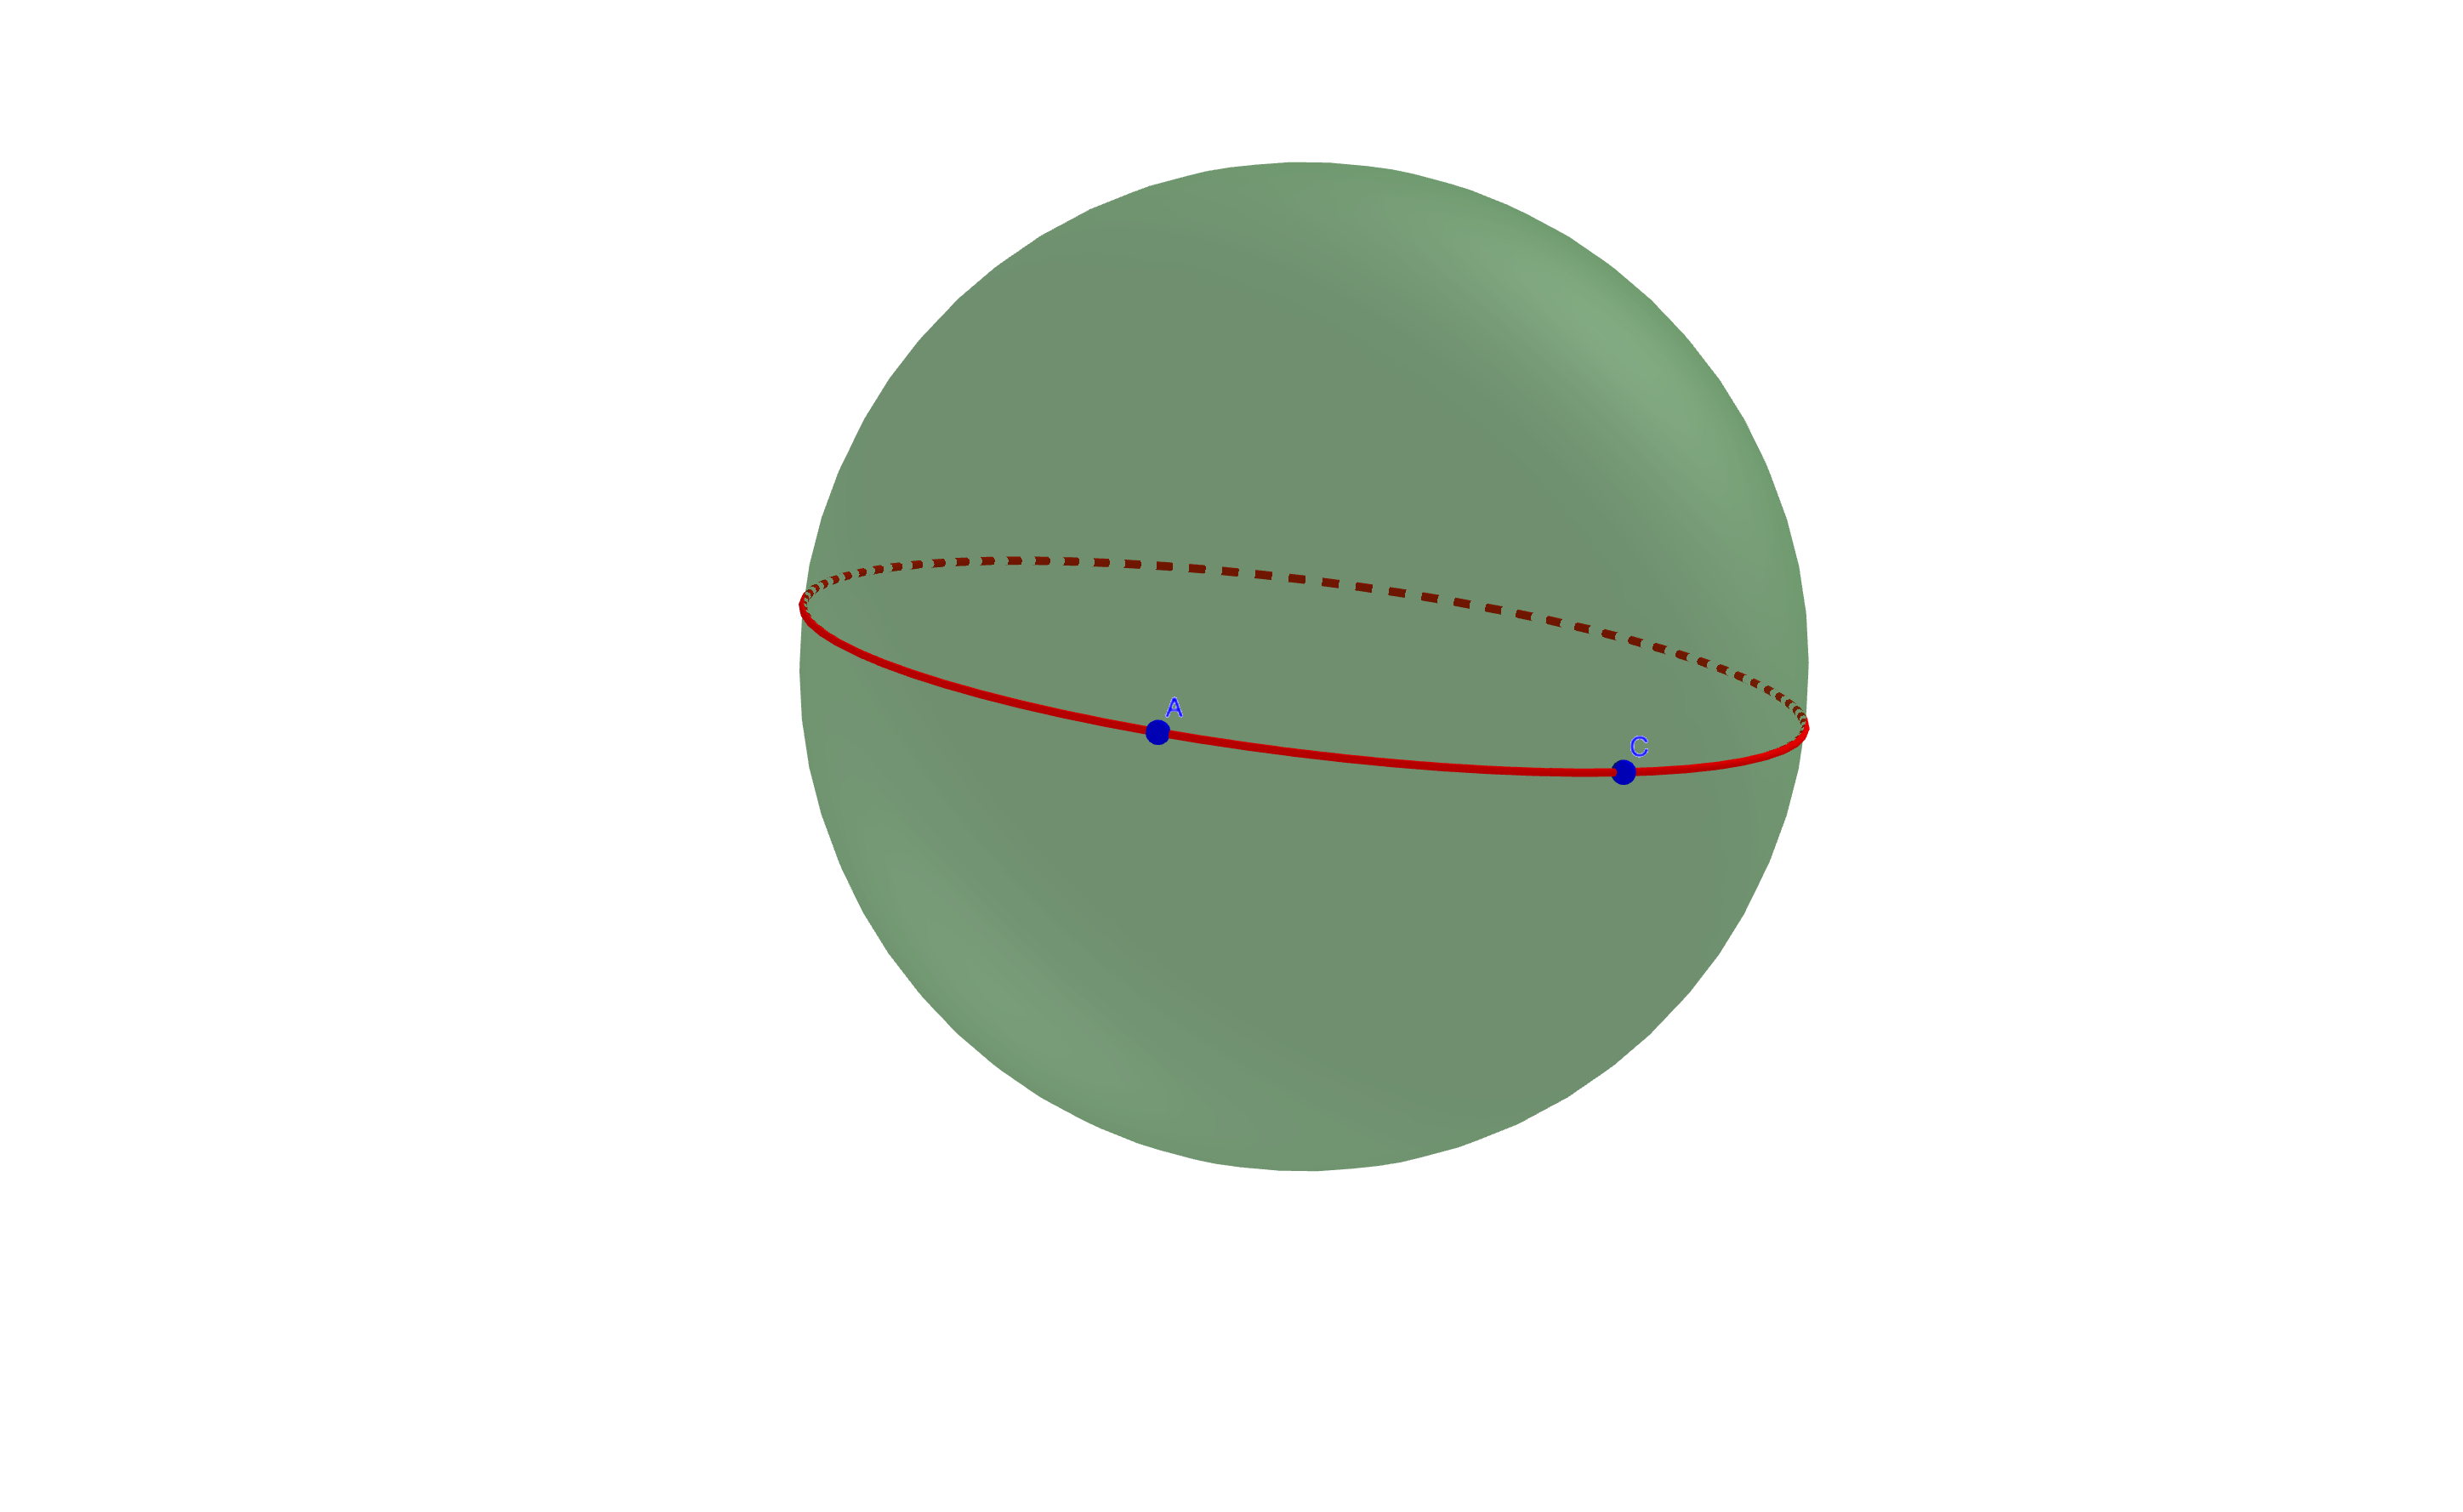
\includegraphics[trim={12cm 12cm 12cm 6cm},clip, width=\textwidth]{oving_1/326.png}
    \end{figure}
  \end{punkt}

  \begin{punkt}
    Dersom $A$ og $C$ er antipodale er $s(A, C)=\pi$ \emph{per definisjon}, ettersom $A$ 
    og $C$ ikke bestemmer en entydig storsirkel. I dette tilfellet er $\overline{AC}$ 
    hele sfæren $S^2$. Hvis vi plukker et tilfeldig punkt $B$ på sfæren, vil $A$, $B$, 
    $C$ alle tre ligge på en felles storsirkel, så det er klart at 
    $s(A,C) = \pi = s(A, B)+s(B, C)$. 
  \end{punkt}
\end{oppgave}



%

\begin{oppgave}[3.2.12]
  At $f:l\longrightarrow \R$ er en koordinatfunksjon betyr at 
  \begin{enumerate}
      \item $PQ=|f(P)-f(Q)|$ for alle punkter $P, Q\in l$. 
      
      \item $f$ er \emph{på}, altså at for alle $x\in \R$ finnes det et punkt $P\in l$ 
      slik at $f(P)=x$.
      
      \item $f$ er 1-til-1, altså at dersom $f(P)=f(Q)$ for to punkter $P, Q\in l$, så
      er $P=Q$. 
  \end{enumerate}
  De to siste punktene betyr at $f$ er en 1-til-1 korrespondanse. 

  \begin{punkt}
    Vi antar at $f$ er en koordinatfunksjon, og dermed tilfredstiler de tre punktene over. 
    Funksjonen er $-f$ er definert ved $(-f)(x)=-f(x)$. For å vite om dette også er en 
    koordinatfunksjon sjekker vi de tre punktene. 
    \begin{enumerate}
        \item Vi har at $|(-f)(P)-(-f)(Q)|=|-f(P)+f(Q)|=|f(P)-f(Q)|$, og siden $f$ er en 
        koordinatfunksjon vet vi at $|f(P)-f(Q)|=PQ$. Altså er $|(-f)(P)-(-f)(Q)| =PQ$. 
        
        \item Velg et tilfeldig punkt $x\in \R$. Siden $f$ er \emph{på}, finnes det et 
        punkt $P$ slik at $f(P)=-x$. Vi har da $(-f)(P) = -f(P)=-(-x)=x$, som viser at 
        også $-f$ er \emph{på}.
        
        \item La $(-f)(P)=(-f)(Q)$. Per definisjon betyr dette at $-f(P)=-f(Q)$, som igjen
        betyr at $f(P)=f(Q)$. Siden $f$ er 1-til-1 betyr dette at $P=Q$. Dermed er også $-f$
        1-til-1. 
    \end{enumerate}
  \end{punkt}

  \begin{punkt}
    Vi antar igjen at $f$ er en koordinatfunksjon. Vi sjekker om $g$ tilfredsstiller de 
    tre punktene. 
    \begin{enumerate}
        \item Vi har $|g(P)-g(Q)|=|f(P)+c - (f(Q)+c)|=|f(P)-f(Q)|$. Siden $f$ er en 
        koordinatfunksjon har vi $|f(P)-f(Q)|=PQ$, og dermed at $|g(P)-g(Q)|=PQ$. 
        \item Velg et tilfeldig punkt $x\in \R$. Siden $f$ er \emph{på} finnes det et 
        punkt $P$ slik at $f(P)=x-c$. Vi har da $g(P)=f(P)+c = x-c+c = x$. Altså er 
        $g$ også \emph{på}. 
        
        \item La $g(P)=g(Q)$. Per definisjon betyr dette at $f(P)+c=f(Q)+c$, som betyr 
        at $f(P)=f(Q)$. Siden $f$ er 1-til-1 betyr dette at $P=Q$. Dermed er også $g$
        1-til-1. 
    \end{enumerate}
  \end{punkt}

  \begin{punkt}
    Anta nå at både $f$ og $h$ er koordinatfunksjoner for $l$. For å vise at to 
    koordinatfunksjoner er like trenger vi faktisk kun å sjekke at de er like i to ulike 
    punkter. La oss se litt nærmere på dette.
    
    \begin{lemma}\label{lm:1}
      La $f$ og $h$ være koordinatfunksjoner for en linje $l$. Dersom $f(P)=h(P)$ og 
      $f(Q)=h(Q)$ for to punkter $P\neq Q$, så er $f(A)=h(A)$ for alle $A\in l$. 
    \end{lemma}

    \begin{proof}
      Anta at $f(P)=h(P)$ og $f(Q)=h(Q)$ der $P\neq Q$. Siden $P\neq Q$ har vi $f(P)\neq f(Q)$.
      Vi kan anta uten ta av generalitet at $f(P)< f(Q)$. La $A\in l$ være et punkt. Vi ønsker 
      å vise at $f(A)=h(A)$. Fra korollar 3.2.19 vet vi at dersom tre ulike punkter ligger på en
      linje, så ligger et av dem mellom de to andre. Vi har nå tre punkter: $P$, $Q$, $A$, og 
      disse kan være i tre konfigurasjoner: $P\ast A\ast Q$, $P\ast Q\ast A$ og $A\ast P\ast Q$. 
      Vi sjekker at $f(A)=h(A)$ i alle tre tilfellene. 
      \begin{enumerate}
        \item $P\ast A\ast Q$: Av teorem 3.2.17 har vi at $f(P)<f(A)<f(Q)$, og fra 
        linjalpostulatet er $$ AQ = |f(Q)-f(A)| = f(Q)-f(A), $$ der vi har fjernet 
        absoluttverditegnet ettersom $f(A)<f(Q)$. Vi har da $f(A)=f(Q)-AQ$. På samme måte får vi 
        $h(A)=h(Q)-AQ$. Dermed har vi $$ f(A)=f(Q)-AQ = h(Q)-AQ = h(A), $$ siden vi har antatt 
        at $f(Q)=h(Q)$. 
    
        \item $P\ast Q\ast A$: De to følgende punktene er så og si helt like som det over, men 
        vi skriver de ut for kompletthets skyld. 
    
        Fra teorem 3.2.17 vet vi at $f(P)<f(Q)<f(A)$, og fra linjalpostulatet er 
        $$ AQ = |f(A)-f(Q)| = f(A)-f(Q), $$ der vi igjen har fjernet absoluttverditegnet siden 
        $f(Q)<f(A)$. Vi har da $f(A)=f(Q)+AQ$. På samme måte får vi $h(A)=h(Q)+AQ$. Dermed har 
        vi $$ f(A)=f(Q)+AQ = h(Q)+AQ = h(A), $$ siden vi har antatt at $f(Q)=h(Q)$. 
    
        \item $A\ast P\ast Q$: Fra teorem 3.2.17 vet vi at $f(A)<f(P)<f(Q)$, og fra 
        linjalpostulatet er $$ AP = |f(P)-f(A)| = f(P)-f(A), $$ der vi igjen har fjernet 
        absoluttverditegnet siden $f(A)<f(P)$. Vi har da $f(A)=f(P)-AP$. På samme måte får 
        vi $h(A)=h(P)+AP$. Dermed har vi $$ f(A)=f(P)-AP = h(P)-AP = h(A), $$ siden vi har 
        antatt at $f(P)=h(P)$. 
      \end{enumerate}
    \end{proof}
    

    Ok, la oss vende tilbake til den faktiske oppgaven. Siden $f$ er en koordinatfunksjon vet 
    vi at det er \emph{på}. Dermed kan vi finne punkter $P$ og $Q$ slik at $f(P)=0$ og $f(Q)=1$.
    Fra linjalpostulatet har vi dermed at $PQ=f(Q)-f(P)=1$. Vi har to muligheter for $h$, enten 
    er $h(P)<h(Q)$, eller så er $h(Q)<h(P)$. Vi ser på den første muligheten først. 

    Anta at $h(P)< h(Q)$. Vi påstår at for en hver $A\in l$ så er $h(A)=f(A)+c$, der $c=h(P)$. Siden 
    $f$ er en koordinatfunksjon vet vi fra b) at funksjonen gitt ved $f(P)+c$ også er en 
    koordinatfunksjon. Fra \cref{lm:1} trenger vi kun å vise at $h(P)=f(P)+c$ og $h(Q)=f(Q)+c$ for 
    å bevise påstanden vår. Vi har $$f(P)+c = f(P)+h(P) = 0+ h(P) = h(P)$$ og 
    \begin{align*}
        f(Q)+c 
        &= f(Q)+h(P) \\
        &= f(Q)+(h(Q)-PQ) \\
        &= h(Q) + (f(Q)-PQ) \\
        &= h(Q),
    \end{align*}
    ettersom $f(Q) = 1 = PQ$. Den andre av likhetene over får vi fra linjalpostulatet. 

    Anta nå at $h(Q)<h(P)$. Vi påstår nå at $h(A)=-f(A)+c$, der igjen $c=h(P)$, for alle $A\in l$.
    Beviset for at dette er sant er helt analogt til det over. Altså, vi sjekker om de er like for 
    $P$ og $Q$, noe som ved \cref{lm:1} betyr at de må være like. Vi har 
    $$h(P)=0+h(P)=-f(P)+c,$$ da $f(P)=0$. Vi har også 
    \begin{align*}
        -f(Q)+c 
        &= -f(Q)+h(P) \\
        &= -f(Q)+(h(Q)+PQ) \\
        &= h(Q) + (PQ-f(Q)) \\
        &= h(Q),
    \end{align*}
    ettersom $f(Q) = 1 = PQ$. Den andre av likhetene over får vi igjen fra linjalpostulatet. 
  \end{punkt}
\end{oppgave}

\begin{oppgave}[3.2.15]
  Oppgaver ber oss om å vise at to mengder er like, altså at 
  $$\overrightarrow{AB} = \{P\in l | f(P)\geq 0\}.$$
  For å vise dette viser vi to ting: først, dersom $P\in \overrightarrow{AB}$ så er $f(P)\geq 0$,
  så, dersom $f(P)\geq 0$ så er $P\in \overrightarrow{AB}$. 
    
  Anta dermed at $P\in \overrightarrow{AB}$. Da har vi enten $P=A$, $P=B$, $A\ast P\ast B$ eller
  $A\ast B\ast P$. Dersom $P=A$ har vi fra beskrivelsen av funksjonen $f$ at $f(P)=0$ og dersom 
  $P=B$ har vi $f(P)>0$. Dersom $A\ast P\ast B$ har vi dermed fra teorem 3.2.17 i boka at 
  $f(A)< f(P)<f(B)$, og dermed at $f(P)\geq 0$. Siste mulighet er at $A\ast B\ast P$, som igjen 
  fra teorem 3.2.17 betyr at $f(A)<f(B)<f(P)$. Alle mulighetene gir oss $f(P)\geq 0$, så vi har 
  vist den første delen. 

  Anta nå at vi har $f(P)\geq 0$. Hvis $f(P)=0$ så har vi $f(A)=f(P)$. Siden $f$ er en-til-en vet 
  vi at dette betyr at $A=P$. Det tilsvarende gjelder dersom $f(P)=f(B)$. I begge tilfeller er
  $P\in \overrightarrow{AB}$. Vi har da to tilfeller igjen, $f(A)<f(P)<f(B)$ og $f(A)<f(B)<f(P)$. 
  Fra teorem 3.2.17 får vi da respektivt at $A\ast P\ast B$ og $A\ast B\ast P$. Dermed er 
  $P\in \overrightarrow{AB}$. 
\end{oppgave}

\begin{oppgave}[3.2.22]
  Vi skal vise at dersom $\overline{AB} = \overline{CD}$, så er enten $A=C$ og $B=D$ eller $A=D$
  og $B=C$. Vi bemerker oss først at $\overleftrightarrow{AB} = \overleftrightarrow{CD}$ ettersom 
  $C$ og $D$ begge ligger på linjen $\overleftrightarrow{AB}$. 

  La nå $f:\overleftrightarrow{AB}\longrightarrow \R$ være en koordinatfunksjon. Vi kan anta uten 
  tap av generalitet at $f(A)<f(B)$ og $f(C)<f(D)$. Fra teorem 3.2.17 får vi to likheter:
    
  $$ \overline{AB}=\{ P|f(A)\leq f(P)\leq f(B) \} $$
  $$ \overline{CD}=\{ P|f(C)\leq f(P)\leq f(D) \} .$$
    
  Siden vi har antatt at $\overline{AB}=\overline{CD}$ vet vi at $C\in \overline{AB}$. Fra den 
  første likheten får vi da at $f(A)\leq f(C)$. Vi vet også at $A\in \overline{CD}$, som fra den 
  andre likheten gir oss $f(C)\leq f(A)$. Siden $f(C)$ er både mindre og større enn $f(A)$ må vi 
  ha $f(A)=f(C)$. Siden $f$ er en-til-en betyr dette at $A=C$. 

  Helt tilsvarende får vi at $B=D$. Merk at mulighetene $A=D$ og $B=C$ forsvant da vi anto at 
  $f(A)<f(B)$ og $f(C)<f(D)$. Snur vi på disse ulikhetene får vi isteden $A=D$ og $B=C$. 
\end{oppgave}

\begin{oppgave}[3.2.24.d)]
  Vi skal vise at $\overline{AB}\cap \overline{BC} = \{B\}$. Siden $A, B, C$ er kolineære finnes en 
  linje $l$ som de alle ligger på. La $f:l\longrightarrow \R$ være en koordinatfunksjon for $l$. 
  Ettersom $B$ ligger mellom $A$ og $C$ vet vi fra teorem 3.2.17 at enten $f(A)<f(B)<f(C)$ eller 
  $f(A)>f(B)>f(C)$. Vi antar $f(A)<f(B)<f(C)$. Beviset vil være helt tilsvarende dersom vi isteden
  antar den andre ulikheten. Fra teorem 3.2.17 får vi to likheter

  $$ \overline{AB}=\{P|f(A)\leq f(P)\leq f(B)\} $$
  $$ \overline{BC})\{P|f(B)\leq f(P)\leq f(C)\} .$$

  Dersom vi tar et punkt $Q\in \overline{AB}\cap \overline{BC}$ må vi fra de to likhetene ha
  $ f(A)\leq f(Q)\leq f(B)$ og $f(B)\leq f(Q)\leq f(C)$. Siden $f(Q)$ er både mindre og større enn 
  $f(B)$ må vi ha $f(Q)=f(B)$. Siden $f$ er en-til-en betyr dette at $Q=B$. 
\end{oppgave}

\begin{oppgave}[3.3.1]
  La $X$ og $Y$ være to konvekse mengder. Vi velger oss to punkter $A$ og $B$ i snittet $X\cap Y$. 
  Dersom vi klarer å vise at linjen $\overline{AB}\subset X\cap Y$, så har vi vist at $X\cap Y$ også 
  er en konveks mengde. 

  Ettersom $A, B\in X\cap Y$ må vi ha $A\in X$, $A\in Y$, $B\in X$ og $B\in Y$. Siden $X$ og $Y$ er 
  konvekse mengder vet vi da at linjen $\overline{AB}\subset X$ og $\overline{AB}\subset Y$. Siden 
  linjen ligger i både $X$ og $Y$ ligger den også per definisjon i snittet av mengdene. Dermed har 
  vi $\overline{AB}\subset X\cap Y$, som var det vi ville vise. 

  Under har vi tegnet et eksempel av to disjunkte konvekse mengder (to disker) $X$ og $Y$. Som vi 
  enkelt kan se, er ikke unionen av disse en konveks mengde. Velg to punkter $A\in X$ og $B\in Y$. 
  Siden $X$ og $Y$ er disjunkte er ikke linjen $\overline{AB}$ inneholdt i $X\cup Y$. Dermed er 
  ikke unionen konveks. 

  \begin{figure}[H]
    \centering
    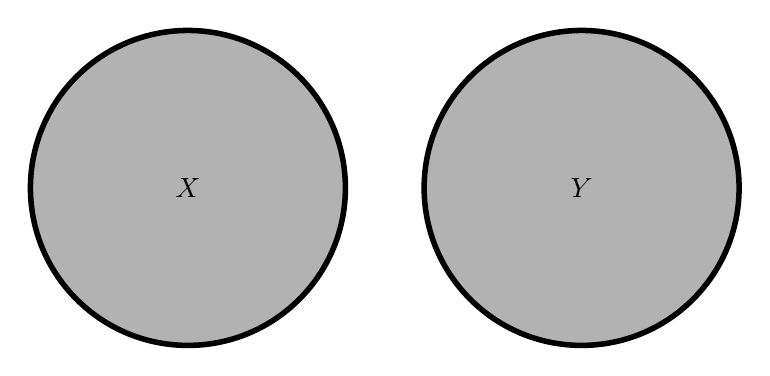
\begin{tikzpicture}
    \draw[fill, black!30] (-2,0) circle (2cm);
    \draw[fill, black!30] (3,0) circle (2cm);
    \draw[black, line width=2pt] (-2,0) circle (2cm);
    \draw[black, line width=2pt] (3,0) circle (2cm);
    \node at (-2,0) {$X$};
    \node at (3,0) {$Y$};
\end{tikzpicture}
  \end{figure}
  
  Vi har to måter å tenke på at den tomme mengden er en konveks mengde. Per definisjon inneholder 
  ikke den tomme mengden noen punkter. Dette betyr at for alle punkter (nettopp ingen) i $\emptyset$ 
  så er linjen mellom de inneholdt i $\emptyset$. Dermed tilfredstiller $\emptyset$ trivielt 
  definisjonen av å være konveks. Vi har i starten av oppgaven også vist at snittet av to konvekse 
  mengder er igjen konvekst. Så, dersom vi tar to disjunkte mengder (for eksempel de vi tegnet over)
  så vil snittet av disse være konvekst. Dette snittet er jo den tomme mengden, så den må da være 
  konveks. 
\end{oppgave}

\begin{oppgave}[3.3.2]
  \begin{itemize}
    \item $\{A\}$: I denne mengden har vi kun ett punkt, nemlig $A$. Så det eneste 
    linjestykket vi har er $\overline{AA}$. Per definisjon har vi 
    $$ \overline{AA} = \{A, A\}\cup \{P|A\ast P\ast A\} = \{A\}. $$
    Ettersom $\{A\}\subseteq \{A\}$ er mengden konveks. 

    \item $\overline{AB}$: La $C$ og $D$ være to punkter i $\overline{AB}$. For at $\overline{AB}$ 
    skal være konvekst må vi vise at linjestykket $\overline{CD}$ er inneholdt i $\overline{AB}$. 
    
    Punktene $A$, $B$, $C$ og $D$ ligger alle på linjen $\overleftrightarrow{AB}$. La 
    $f:\overleftrightarrow{AB}\longrightarrow \R$ være en koordinatfunksjon, som vi fra teorem 
    3.2.16 kan anta at oppfyller $f(A)=0$ og $f(B)>0$. Vi antar videre uten tap av generalitet at 
    $f(C)<f(D)$. Fra teorem 3.2.17 får vi to likheter

    $$ \overline{AB}=\{P|f(A)\leq f(P)\leq f(B)\} $$
    $$ \overline{CD}=\{P|f(C)\leq f(P)\leq f(D)\} .$$

    Siden $C, D\in \overline{AB}$ vet vi dermed at $f(A)\leq f(C)\leq f(D)\leq f(B)$. Dette betyr 
    også at for et hvert punkt $P\in \overline{CD}$ så har vi $f(A)\leq f(P)\leq f(B)$. Fra teorem
    3.2.17 vet vi da at $A\ast P\ast B$, som vil si at $P\in \overline{AB}$. Dermed har vi 
    $\overline{CD}\subseteq \overline{AB}$.  

    \item $\overrightarrow{AB}$: Som over lar vi $f:\overleftrightarrow{AB}\longrightarrow \R$ være
    en koordinatfunksjon slik at $f(A)=0$ of $f(B)>0$. Velg to punkter $C, D \in \overrightarrow{AB}$
    med $f(C)<f(D)$. Vi vil vise at $\overline{CD}\subset \overrightarrow{AB}$. 
    
    Siden $C, D\in \overrightarrow{AB}$ vet vi at $f(C)\geq 0$ og $f(D)\geq 0$. Fra teorem 3.2.17
    får vi likheten

    $$ \overline{CD} = \{P| f(C)\leq f(P)\leq f(D)\},$$

    som betyr at $f(P)\geq f(C)\geq 0$ for alle punkter $P\in \overline{CD}$. Siden 
    $\overrightarrow{AB} = \{P|0\leq f(P)\}$ får vi at $P\in \overleftrightarrow{AB}$ for alle 
    punkter $P\in \overline{CD}$, som betyr at $\overline{CD}\subset \overrightarrow{AB}$. 

    \item $\overleftrightarrow{AB}$: Velg to punkter $C$ og $D$ på $\overleftrightarrow{AB}$. Vi vil
    vise at $\overline{CD}\subset \overleftrightarrow{AB}$. 

    For et punkt $P\in \overline{CD}$ har vi enten $P=C$, $P=D$ eller $C\ast P\ast D$. I de to 
    første tilfellene har vi åpenbart $P\in \overleftrightarrow{AB}$. Dersom $C\ast P\ast D$ så må 
    $C$, $P$ og $D$ ligge på en felles linje $l$. Siden to punkter ligger på en \emph{unik} linje, 
    og $C$ og $D$ ligger på både $l$ og $\overleftrightarrow{AB}$ må vi ha $l=\overleftrightarrow{AB}$.
    Dermed har vi $P\in \overleftrightarrow{AB}$ som betyr at 
    $\overline{CD}\subset \overleftrightarrow{AB}$, som var det vi ville vise. 

  \end{itemize}
\end{oppgave}

\begin{oppgave}[3.3.4]
  \begin{punkt}
    Vi må vise at modellen tilfredstiller alle punktene i aksiom 3.3.2. Vi tolker her storsirkel som
    linje og halvsfære som halvplan. Det er klart at en storsirkel $l$ deler sfæren inn i to halvsfærer
    $H_1$ og $H_2$, og at disse er ikke-tomme og disjunkte. 

    Vi vil vise at $H_1$ og $H_2$ er konvekse. Anta at $A$ og $B$ er to punkter i $H_1$. Vi må altså 
    vise at linjestykket $\overline{AB}\subset H_1$. Merk at siden $A$ og $B$ ligger i samme halvsfære
    kan de ikke være antipodale. Dermed kan vi bruke (som vist i øving 1, oppgave 3.2.6(a)) at
    $\overline{AB}$ er den korteste delbuen mellom $A$ og $B$ langs den unike storsirkelen bestemt av 
    $A$ og $B$. Denne delbuen ligger i $H_1$, så $H_1$ er en konveks mengde. Tilsvarende viser at $H_2$
    er konveks. 

    La $C\in H_1$ og $D\in H_2$ har vi to muligheter: 
    \begin{enumerate}
      \item $C$ og $D$ er antipodale. Dette vil si at $\overline{CD} = S^2$, som vil si at
      $\overline{CD}\cap l = l$. 

      \item $C$ og $D$ er ikke antipodale. Siden $C$ og $D$ ligger i forskjellige halvsfærer vil 
      enhver sti fra $C$ til $D$ krysse $l$, spesielt vil dette gjelde for $\overline{CD}$. 
    \end{enumerate}

    I begge tilfellene er snittet $\overline{CD}\cap l\neq \emptyset$. Oppgaven kan oppsummeres med
    følgende figur: 
    \begin{figure}[H]
      \centering 
      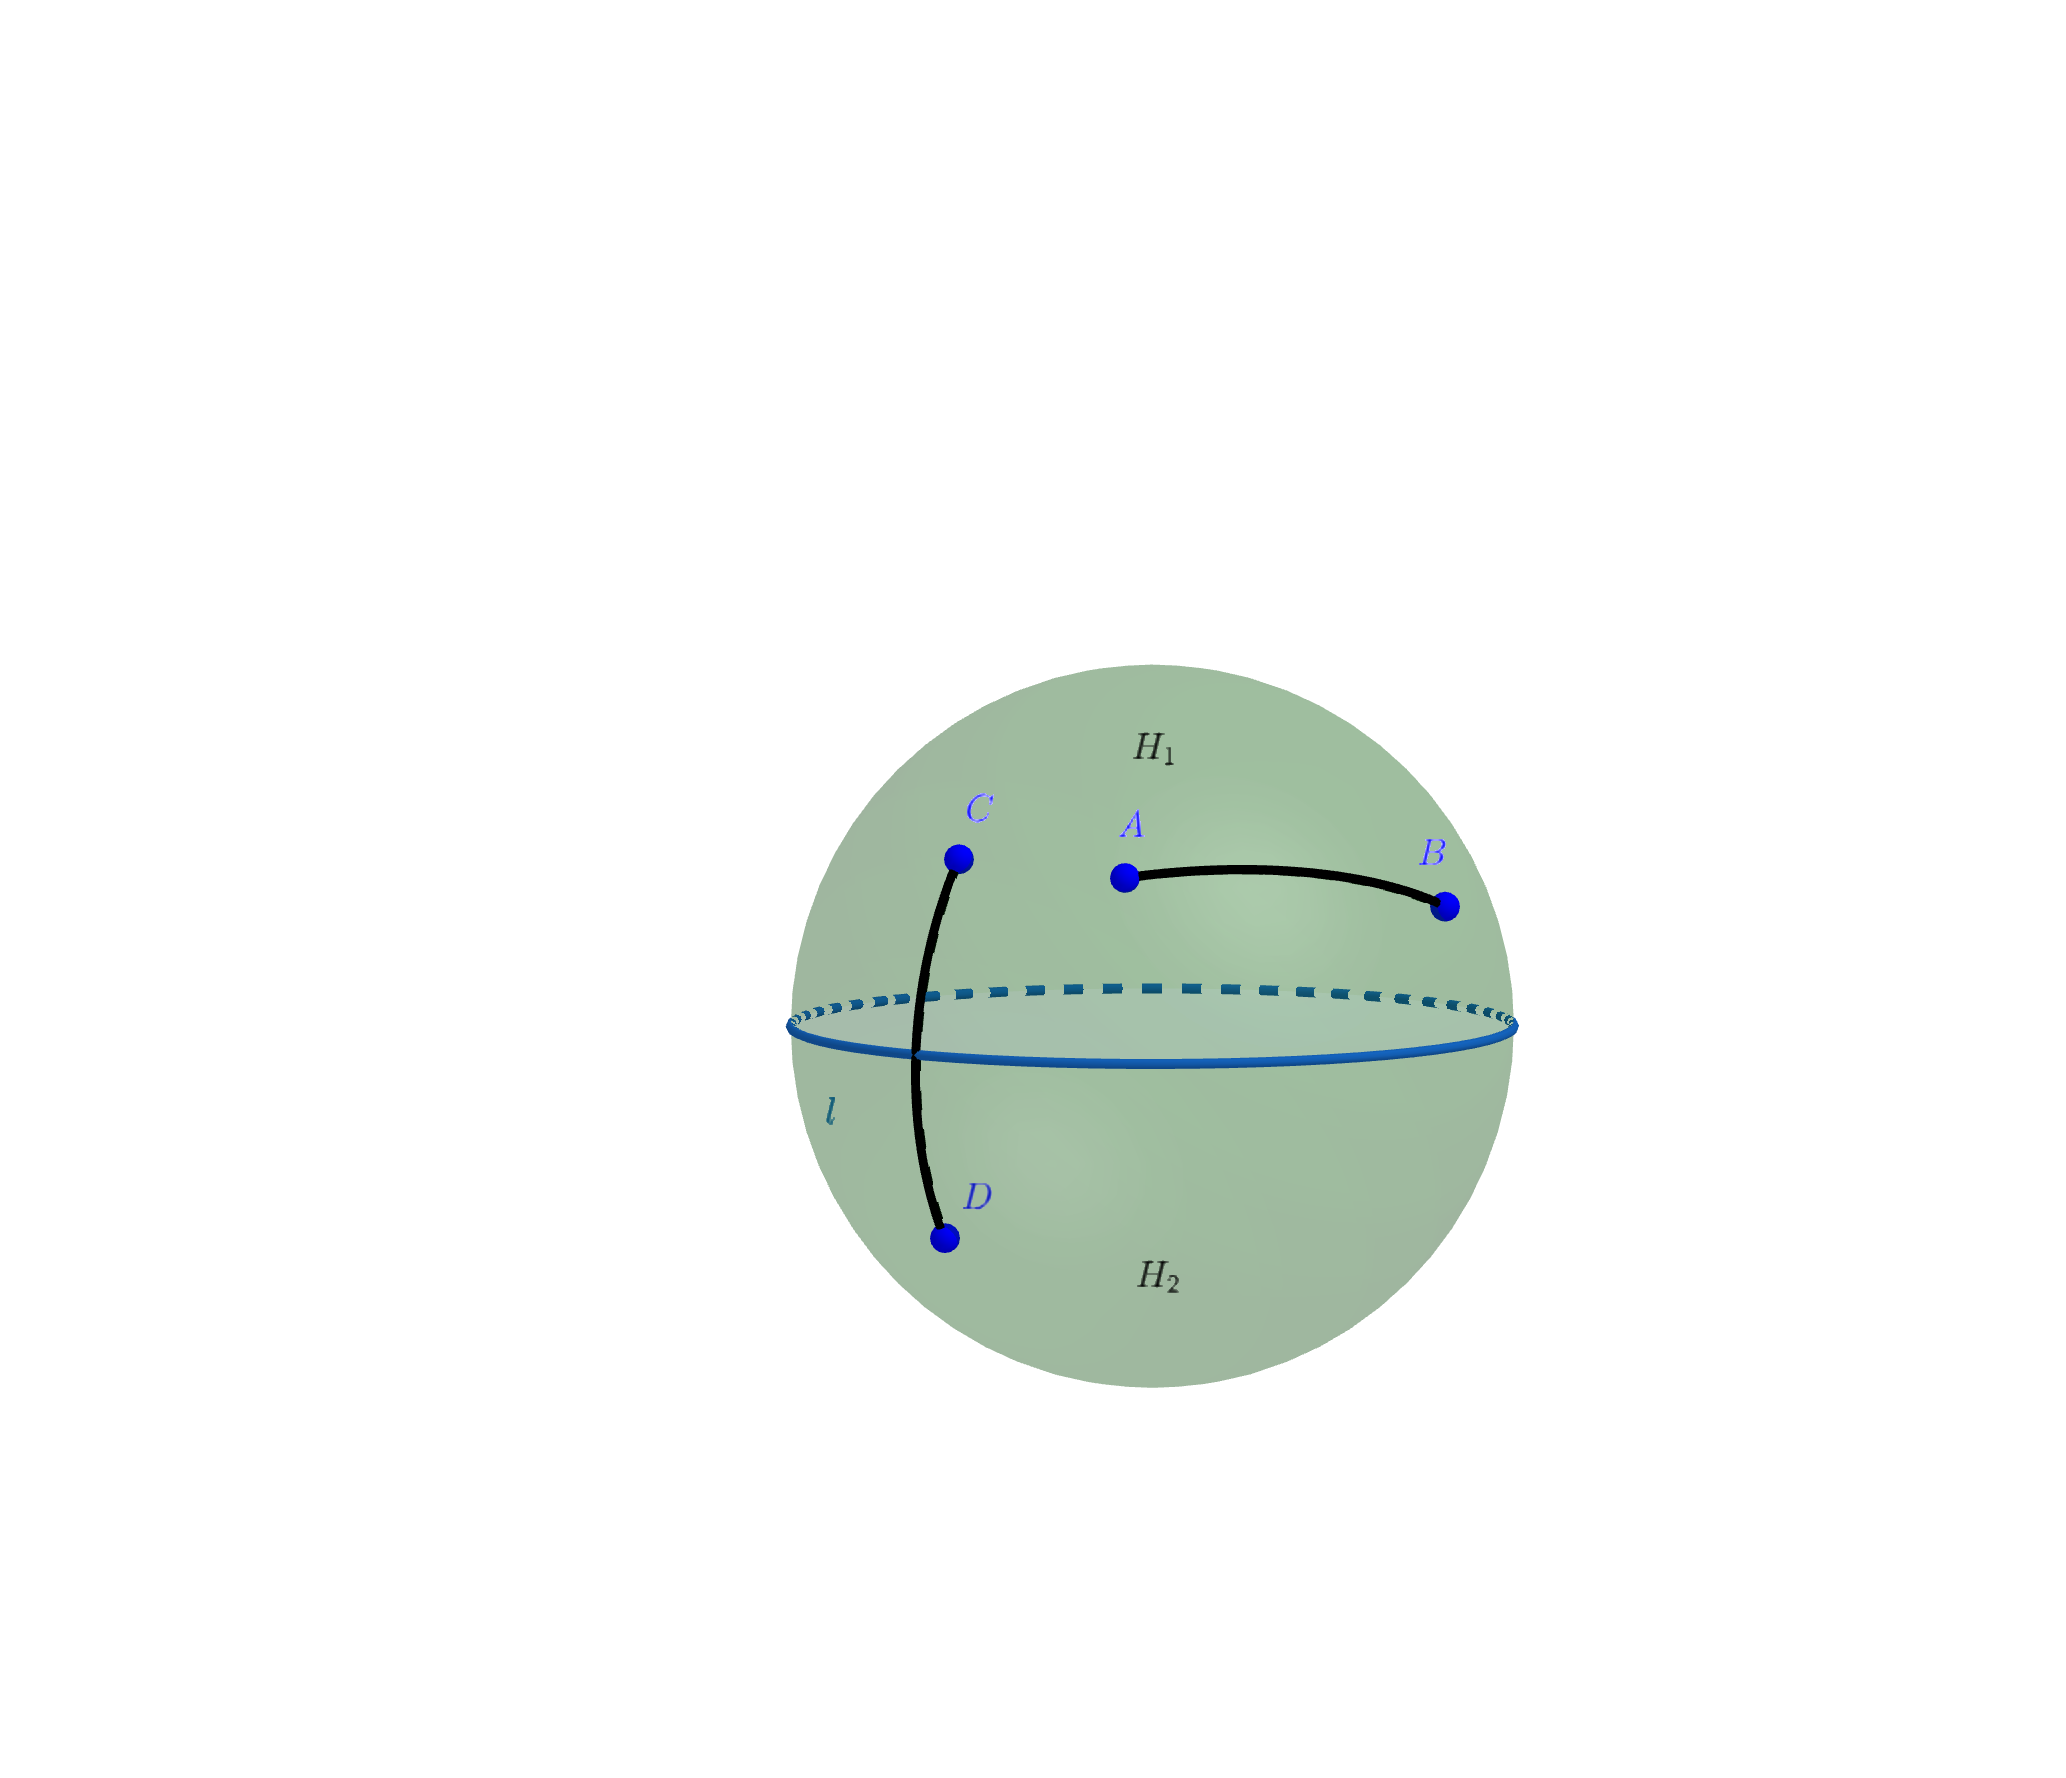
\includegraphics[trim={13cm 13cm 12cm 22cm},clip, width=0.9\textwidth]{oving_2/334a.png}
    \end{figure}
    
  \end{punkt}

  \begin{punkt}
    Vi vet fra øving 1 at $A\ast B\ast C$ hvis og bare hvis $A, B, C$ ligger på samme storsirkel og 
    $s(A, B)+s(B,C) = s(A,C)$. La nå $l$ være storsirkelen bestemt av $A$ og $B$. På en litt uformell
    måte kan vi si at $s(A, B)+s(B, C) = s(A, C)$ dersom korteste vei mellom $A$ og $C$ på storsirkelen
    $l$ går gjennom $B$. Dette skjer når $C$ ligger på den \emph{halve storsirkelen} bestemt av $A$ og 
    $B$ -- se figuren under. Merk at både $A$ og dets antipodale punkt $D$ ligger på strålen. 

    \begin{figure}[H]
      \centering 
      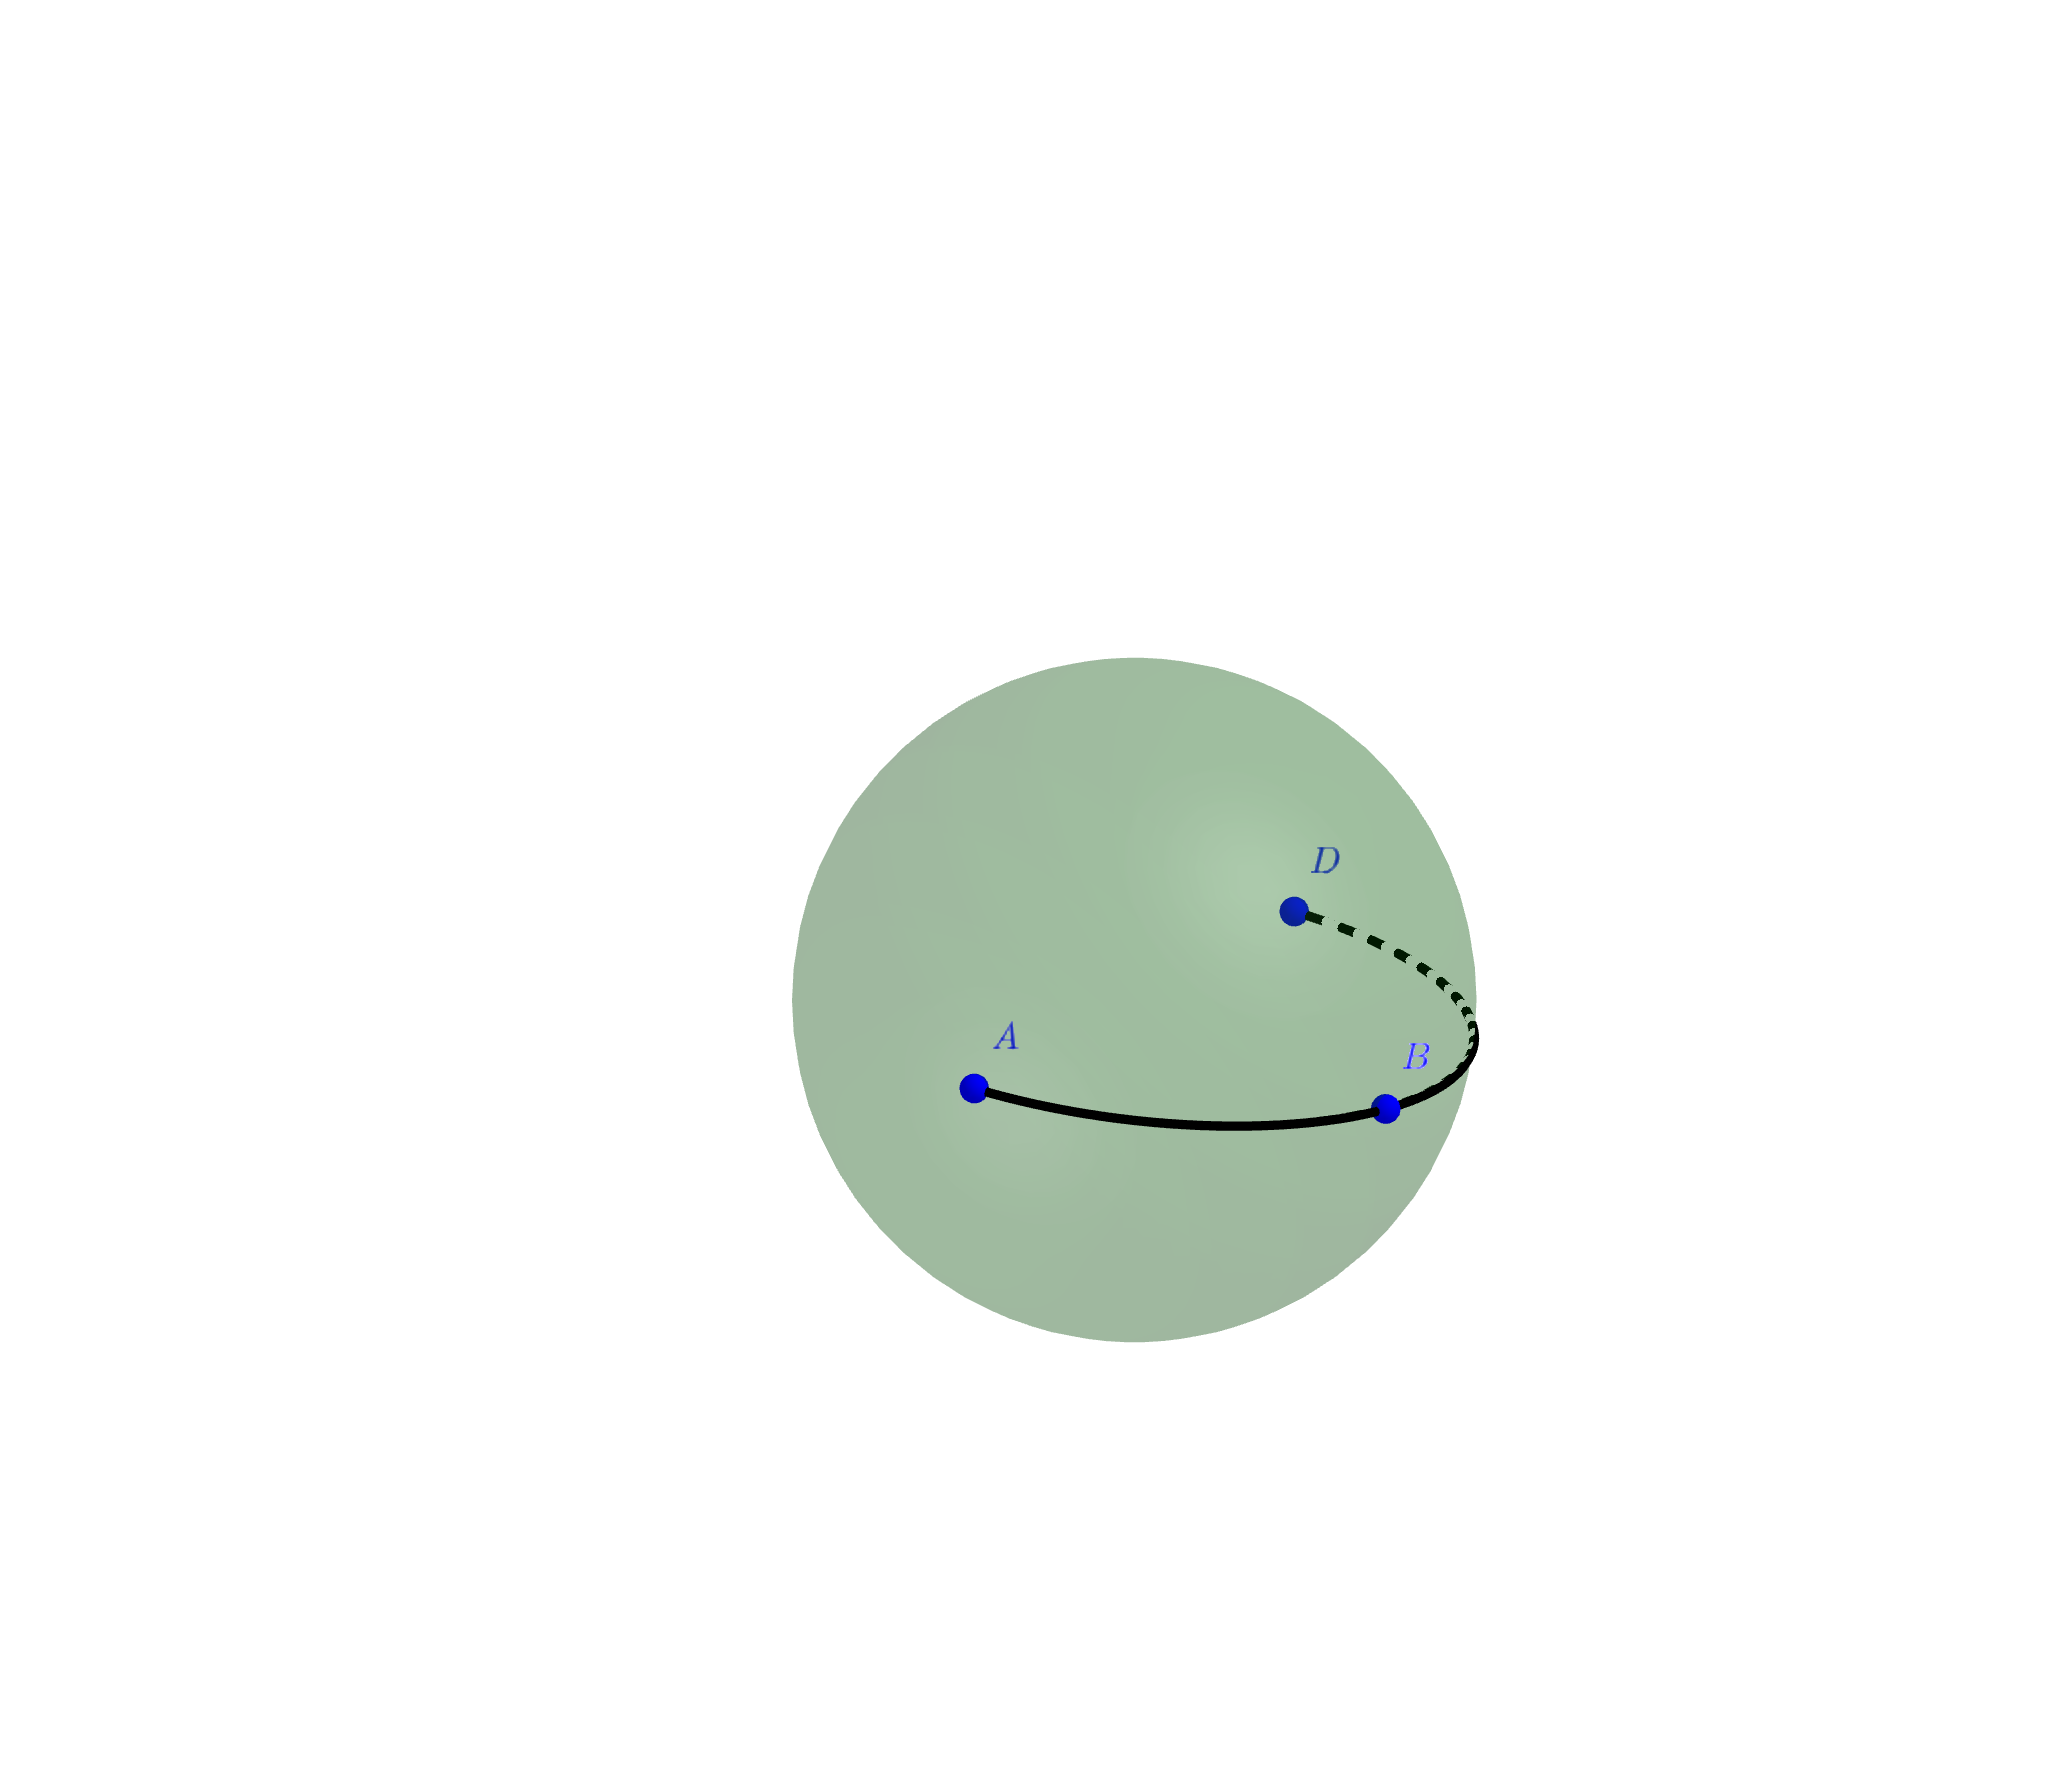
\includegraphics[trim={13cm 13cm 12cm 22cm},clip, width=0.9\textwidth]{oving_2/334b.png}
    \end{figure}
  \end{punkt}

  \begin{punkt}
    Nei, teorem 3.3.9 holder ikke her. Hvis vi lar $D$ være det antipodale punktet til $A$, ligger $D$
    på strålen $\overrightarrow{AB}$ fra deloppgave b). Men, $B$ og $D$ ligger ikke begge på en felles
    side av storsirkelen $l$, ettersom $D$ ligger \emph{på} storsirkelen $l$. Se figuren under.

    \begin{figure}[H]
      \centering 
      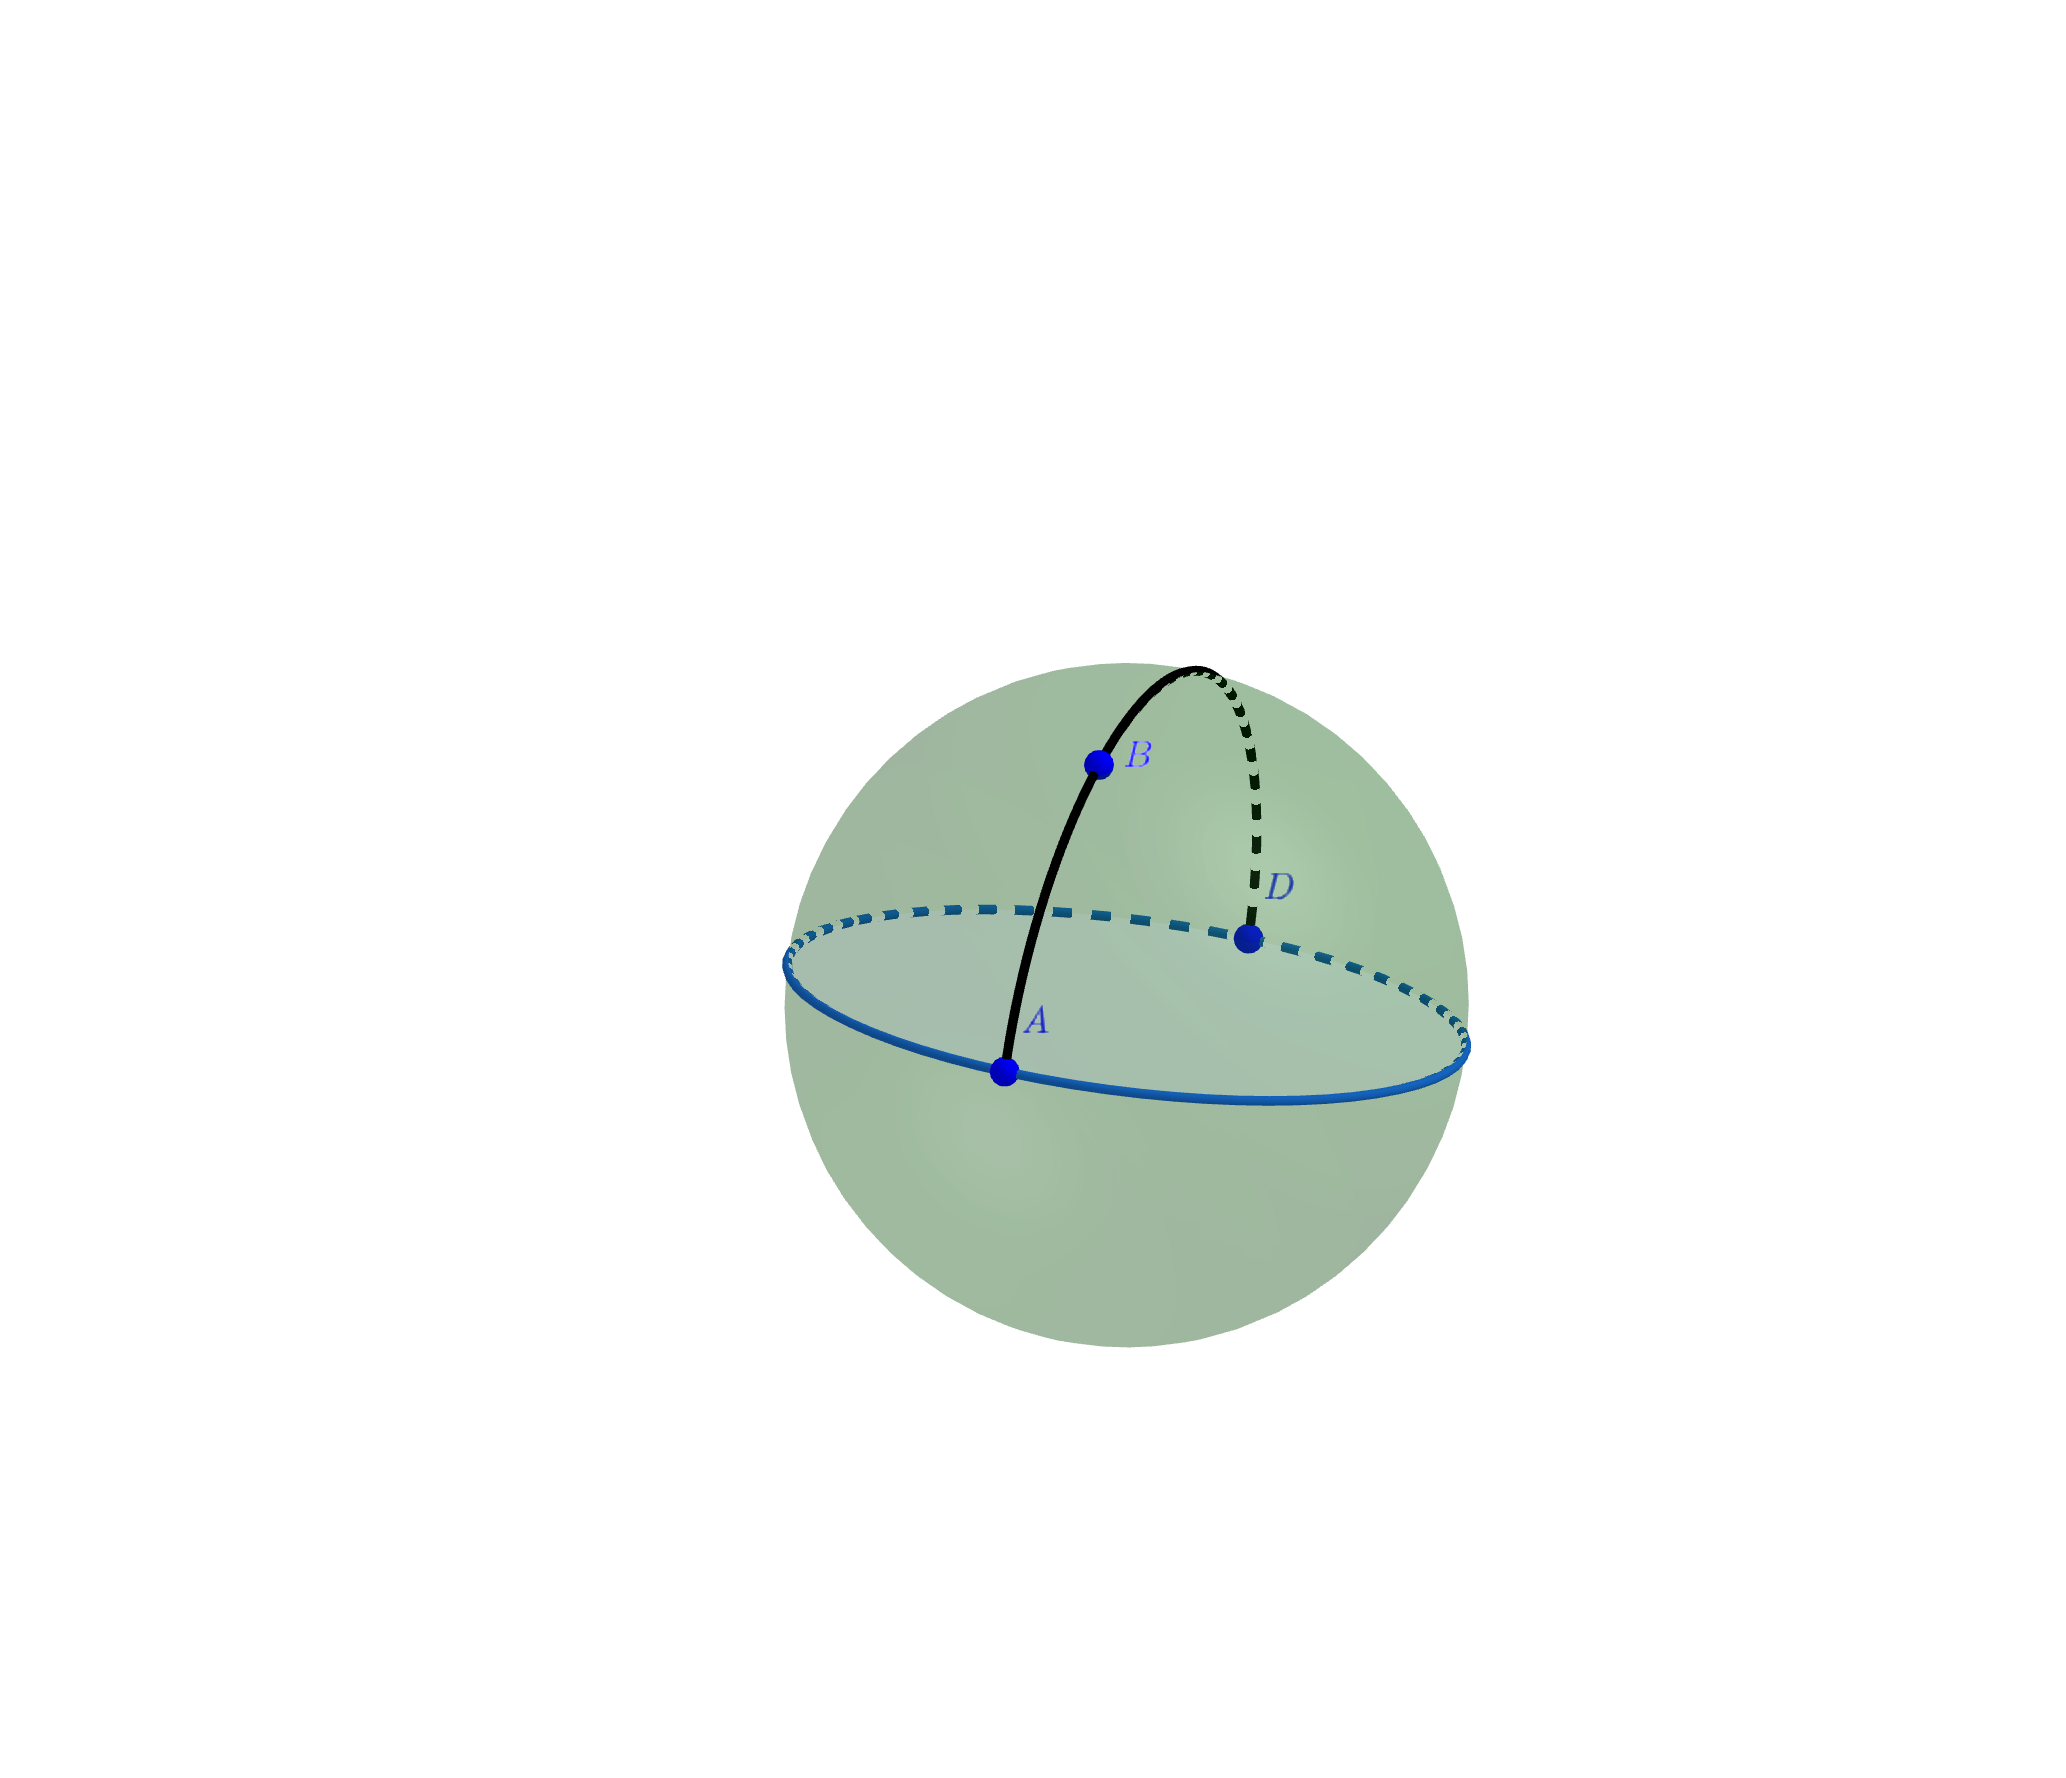
\includegraphics[trim={13cm 13cm 12cm 23cm},clip, width=0.9\textwidth]{oving_2/334c.png}
    \end{figure}
  \end{punkt}
\end{oppgave}

\begin{oppgave}[3.3.5]
  Fra planseparasjonsaksiomet deler linjen $l$ resten av planet i to halvplan $H_1$ og $H_2$. 
  Siden ingen av hjørnene $A$, $B$, $C$ ligger på $l$ må de ligge enten i $H_1$ eller 
  $H_2$. Vi har da tre punkter fordelt på to halvplan, som vil si at minst to av de må ligge i samme
  halvplan. Vi antar uten tap av generalitet at disse to punktene er $A$ og $B$, og at de ligger i 
  $H_1$. Siden $H_1$ er en konveks mengde, vil også linjestykket $\overline{AB}$ ligge i $H_1$. Dette
  betyr at ingen av punktene på $\overline{AB}$ ligger på $l$, så $l$ skjærer ikke siden $\overline{AB}$
  i trekanten. 

  Det er fult mulig for en linje å skjære trekanten $\triangle ABC$ i alle tre sidene. Linjen 
  $\overleftrightarrow{AB}$ vil skjære $\overline{AB}$ i punktet $A$, $\overline{BC}$ i punktet $B$ og 
  $\overline{AC}$ i punktet $A$. 

\end{oppgave}
 


%
\begin{oppgave}[3.4.1]
    La $A$, $B$, $C$ være tre punkter som ikke ligger på en linje. Vi skal finne et punkt $D$ som 
    ligger i det indre av $\angle BAC$ slik at $\mu(\angle BAD)=\mu(\angle DAC)$. La $H_C$ være 
    halvplanet bestemt av linje $\overleftrightarrow{AB}$ og punktet $C$. 
    
    Av tredje del av gradskivepostulatet (aksiom 3.4.1) finnes det en unik stråle $\overrightarrow{AD}$ 
    slik at $D$ ligger i $H_C$ og $\mu(\angle BAD) = \frac{\mu(\angle BAC)}{2}$. Siden 
    $\mu(\angle BAD) < \mu(\angle BAC)$, gir teorem 3.4.5 at $\overrightarrow{AD}$ ligger mellom strålene
    $\overrightarrow{AB}$ og $\overrightarrow{AC}$, som per definisjon betyr at $D$ ligger i det indre av
    $\angle BAC$. Av del 4 av gradskivepostulatet (vinkeladdisjonspostulatet) er 
    $$\mu(\angle BAC) = \mu(\angle BAD)+\mu(\angle DAC),$$
    og siden $\mu(\angle BAD) = \frac{\mu(\angle BAC)}{2}$ per konstruksjon må 
    $\mu(\angle BAD) = \mu(\angle DAC) = \frac{\mu(\angle BAC)}{2}$. 
    
    Siden strålen $\overrightarrow{AD}$ er unik av del tre av gradskivepostulatet, har vi også vist 
    unikhetsdelen av utsagnet. 
\end{oppgave}

\begin{oppgave}[3.4.2]
    \begin{punkt}
        Vi må vise at $f$ er injektiv (\emph{en-til-en}) og surjektiv (\emph{på}). 
        
        \textbf{Surjektiv:} La $c\in (0, 180)$ være gitt. Av del tre av gradskivepostulatet finnes en 
        stråle $\overrightarrow{AE}$ slik at $E\in H$ og $\mu(\angle BAE) = c$. Med andre ord er 
        $f(\angle BAE)=c$, som viser at $f$ er surjektiv. 

        \textbf{Injektiv:} Anta at $\mu(\angle BAD) = \mu(\angle BAE)$ for 
        $\angle BAD, \angle BAE \in \mathcal{A}$. For et hvert tall $r\in (0, 180)$ sier del tre av 
        gradskivepostulatet at det finnes en \emph{unik} stråle $\overrightarrow{AE}$ alik at 
        $\mu(\angle BAE)=r$, og unikhetsdelen gir oss at $\overrightarrow{AE}=\overrightarrow{AD}$ 
        ettersom $\mu(\angle BAD) = \mu(\angle BAE)$. Da vi har definert en vinkel som unionen av to stråler
        får vi at 
        $$ \angle BAE 
        = \overrightarrow{AB}\cup \overrightarrow{AE}
        = \overrightarrow{AB}\cup \overrightarrow{AD} 
        = \angle BAD, $$
        som viser at $f$ er injektiv. 
    \end{punkt}

    \begin{punkt}
        Av teorem 3.4.5 vet vi at $\overrightarrow{AF}$ ligger mellom strålene $\overrightarrow{AB}$ og 
        $\overrightarrow{AE}$ hvis og bare hvis $\mu(\angle BAF)<\mu(\angle BAE)$. Men vi har definert 
        $f(\angle BAF)=\mu(\angle BAF)$ og $f(\angle BAE)=\mu(\angle BAE)$. Derfor har vi 
        $\mu(\angle BAF)<\mu(\angle BAE)$ hvis og bare hvis $f(\angle BAF)<f(\angle BAE)$, 
        som beviser utsagnet. Vi burde også egentlig argumentere for at $f(\angle BAF)>0$, men dette 
        følger direkte fra gradskivepostulatet. 
    \end{punkt}
\end{oppgave}

\begin{oppgave}[3.5.1]
    Det at $m\perp l$ betyr per definisjon at det finnes et punkt $A$ som ligger på både $m$ og $l$, og 
    to punkter $B\in l$, $C\in m$ slik at $\mu(\angle BAC) = 90$. Ved hjelp av linjalpostulatet kan vi 
    finne et punkt $D$ på $l$ og et punkt $E$ PÅ $m$ slik at $D\ast A\ast B$ og $E\ast A\ast C$. Da er 
    $\overrightarrow{AB}$ og $\overrightarrow{AD}$ motsatte stråler, så vi kan anvende teorem 3.5.5 som 
    gir oss at 
    $$ \mu(\angle BAC)+\mu(\angle CAD) = 180 .$$
    Siden vi vet at $\mu(\angle BAC)=90$, må vi også ha $\mu(\angle CAD)=90$. Helt tilsvarende kan man 
    vise at $\mu(\angle DAE)=\mu(\angle EAB) = 90$, slik at de fire strålene $\overrightarrow{AB}$, 
    $\overrightarrow{AC}$, $\overrightarrow{AD}$ og $\overrightarrow{AE}$ står vinkelrett på hverandre. 
\end{oppgave}

\begin{oppgave}[3.5.2]
    Vi viser først eksistens, og så unikhet. 

    \textbf{Eksistens:} La $l$ være en linje og $A$ et punkt på $l$. Vi velger et annet punkt $B$ på 
    $l$, slik at $\overleftrightarrow{AB}=l$. Fra planseparasjonsaksiomet deler linjen planet inn i to 
    halvplan $H_1$ og $H_2$ -- vi velger å bruke $H_1$ her, men kunne like gjerne 
    brukt $H_2$. Fra gradskivepostulatet finnes det for etthvert reellt tall $r$ mellom $0$ og $180$
    en unik stråle $\overrightarrow{AE}$ slik at $E\in H_1$ og $\mu(\angle BAE)=r$. Ved å velge 
    $r =  90$ får vi at linjen $\overleftrightarrow{AE}$ er perpendikulær på linjen 
    $\overleftrightarrow{AB}$. Altså eksisterer det en linje $m$ slik at $A\in m$ og $m\perp l$. 

    \textbf{Unikhet:} Anta at vi har to linjer $m$ og $m'$ slik at de begge er perpendikulære til $l$ og
    at punktet $A$ ligger på både $m$ og $m'$. Fra definisjonen av å være perpendikulær, finnes det to 
    punkter $B$ og $B'$ på $l$, et punkt $C\in m$ og et punkt $C'\in m'$, slik at 
    \begin{enumerate}[label=\arabic*)]
        \item $\mu(\angle BAC)=90$
        \item $\mu(\angle B'AC')=90$.
    \end{enumerate}
    Vi har da to muligheter. Linjen $l$ deler ved planseparasjonsaksiomet planet inn i to halvplan 
    $H_1$ og $H_2$, så enten ligger punktene $C$ og $C'$ i samme halvplan, eller så ligger de i 
    ulike halvplan. Dersom de ligger i samme halvplan, for eksempel $H_1$, vet vi fra 
    gradskivepostulatet at strålen $\overrightarrow{AC}$ som danner vinkelen $\mu(\angle BAC)$ er unik. 
    Dermed må vi ha $\overrightarrow{AC}=\overrightarrow{AC'}$, som vil si at linjene $m$ og $m'$ deler
    to punkter -- ergo er de like. Dersom $C$ og $C'$ ligger i ulike halvplan er strålene 
    $\overrightarrow{AC}$ og $\overrightarrow{AC'}$ motsatte stråler. Dermed er 
    $m=\overleftrightarrow{AC}=\overleftrightarrow{AC'}=m'$, som viser at linjene er de samme. 
    
    Altså finnes det for enhver linje $l$ og et punkt $A$ på $l$, en unik linje $m$ slik at $A\in m$ og 
    $l\perp m$.  
\end{oppgave}

\begin{oppgave}[3.5.3]
    La $A$ og $B$ være ulike punkt. Vi må vise at det finnes en unik linje $m$ slik at midtpunktet $M$ av 
    $\overline{AB}$ ligger på $m$ og $\overleftrightarrow{AB}\perp m$. Fra teorem 3.2.22 vet vi at 
    midtpunktet $M$ finnes og er unikt. Fra forrige oppgave vet vi at det finnes en unik linje $m$ som 
    går gjennom $M$ og er perpendikulær til $\overleftrightarrow{AB}$. Denne linja tilfredsstiller alle
    kravene våre, og må være unik fordi både midtpunktet og linjen er det. 
\end{oppgave}

\begin{oppgave}[3.5.4]
    La $\angle ABC$, $\angle DEF$, $\angle GHI$ og $\angle JKL$ være fire vinkler slik at 
    \begin{enumerate}[label = \arabic*)]
        \item $\angle ABC$ og $\angle DEF$ er supplementærvinkler
        \item $\angle GHI$ og $\angle JKL$ er supplementærvinkler
        \item $\angle DEF \cong \angle JKL$. 
    \end{enumerate}
    Vi må vise at $\angle ABC \cong \angle GHI$. 

    Fra punkt 1) og 2) vet vi at $\mu(\angle ABC)+\mu(\angle DEF) = 180$ og 
    $\mu(\angle GHI)+\mu(\angle JKL) = 180$. Fra punkt 3) vet vi at $\mu(\angle DEF)=\mu(\angle JKL)$. 
    Vi har dermed 
    \begin{align*}
        \mu(\angle ABC)+\mu(\angle DEF) 
        &= 180 \\
        &= \mu(\angle GHI)+\mu(\angle JKL) \\
        &= \mu(\angle GHI)+ \mu(\angle DEF)
    \end{align*} 
    Ved å trekke fra $\mu(\angle DEF)$ i ligningen står vi igjen med $\angle ABC \cong \angle GHI$, 
    som var det vi ville vise. 
\end{oppgave}

\begin{oppgave}[3.5.5]
    Vi ønsker å vise at dersom to vinkler $\angle BAC$ og $\angle DAE$ er slik at 
    \begin{enumerate}[label=\arabic*)]
        \item $\overrightarrow{AB}$ og $\overrightarrow{AE}$ er motsatte stråler,
        \item $\overrightarrow{AC}$ og $\overrightarrow{AD}$ er motsatte stråler,
    \end{enumerate}
    så er $\mu(\angle BAC)=\mu(\angle DAE)$. 

    Siden $\overrightarrow{AB}$ og $\overrightarrow{AE}$ er motsatte stråler, gir teorem 3.5.5 oss at 
    $\mu(\angle BAC)+\mu(\angle CAE)=180$, altså at de er supplementære. Helt tilsvarende får vi at 
    $\mu(\angle CAE)+\mu(\angle DAE)=180$. Ved å trekke den andre likningen fra den første får vi 
    $$\mu(\angle BAC)-\mu(\angle DAE) = 0,$$
    som gir oss det vi ønsket: $\mu(\angle BAC)=\mu(\angle DAE)$. 
\end{oppgave}

\begin{oppgave}[3.5.6]
    Fra linjalpostulatet har vi et punkt $F$ på $\overleftrightarrow{DB}$ slik at $F\ast B\ast D$. Siden
    $\overrightarrow{BD}$ og $\overrightarrow{BF}$ er motsatte stråler, kan vi bruke teorem 3.5.13 til å
    konkludere med at $\mu(\angle DBC)=\mu(\angle ABF)$. Siden vi antar at 
    $\mu(\angle DBC)=\mu(\angle ABE)$, har vi $$\mu(\angle ABE)=\mu(\angle ABF).$$
    Fra konstruksjonen vår vet vi at $E$ og $F$ ligger op samme side av $\overleftrightarrow{AB}$. 
    Resultatet følger nå fra unikhetsdelen av punkt 3) i gradskivepostulatet, altså: siden 
    $\mu(\angle ABE)=\mu(\angle ABF)$ og $E$ og $F$ ligger på samme side av $\overleftrightarrow{AB}$, 
    må $\overrightarrow{BE}=\overrightarrow{BF}$. Siden $\overrightarrow{BF}$ og $\overrightarrow{BD}$ 
    er motsatte stråler får vi at også $\overrightarrow{BD}$ og $\overrightarrow{BE}$ er motsatte 
    stråler, som var det vi skulle vise. 
\end{oppgave}
%
\begin{oppgave}[3.6.1]
    La $A$, $B$, $C$, være tre punkter som ikke ligger på linje. Vi skal finne en stråle $\overrightarrow{AB}$ slik at $M$ ligger i det indre av vinkelen $\angle BAC$ og $\mu(\angle BAM)=\mu(\angle MAC)$.
    Vi bruker først teorem 3.2.23 til å finne et punkt $C'$ på $\overrightarrow{AC}$ slik at $AB=AC'$. 
    Vi bruker så teorem 3.2.22 til å finne midtpunktet $M$ på linjestykket $\overline{BC'}$.
    Det at punktet $M$ ligger i det indre av vinkelen vår får vi fra teorem 3.3.10. 
    Rent intuitivt burde strålen $\overrightarrow{AM}$ være vinkelhalveringsstrålen vi søker, og vi skal nå vise at dette faktisk stemmer. 

    Trekanten $\triangle ABC$ er likebeint per konstruksjon, og av teorem 3.6.5 følger det at $\angle BC'A \cong \angle C'BA$. 
    Nå kan vi bruke side-vinkel-side postulatet på trekantene $\triangle ABM$ og $\triangle AMC'$ til å konkludere med at $\triangle ABM \cong \triangle AMC'$. 
    Dette betyr da spesielt at vi har $\mu(\angle BAM) = \mu(\angle MAC')$.
    Siden $C'$ ligger på strålen $\overrightarrow{AC}$ har vi også $\mu(\angle MAC') = \mu(\angle MAC)$.
    Dermed kan vi konkludere med at $\mu(\angle BAM) = \mu(\angle MAC)$, som viser at $\overrightarrow{AM}$ er en vinkelhalveringsstråle til vinkelen. 

    Unikhet følger ettersom både punktet $C'$ og midtpunktet $M$ er unike. 

    \begin{figure}[H]
        \centering
        

\definecolor{qqqqff}{rgb}{0,0,1}
\begin{tikzpicture}[line cap=round,line join=round,>=triangle 45,x=1cm,y=1cm]
\clip(-5,-1.6) rectangle (6,5);
\draw [shift={(2.580611412565809,2.558493359853798)},line width=2pt,color=qqqqff,fill=qqqqff,fill opacity=0.10000000149011612] (0,0) -- (-145.91991251835023:0.5433730839157709) arc (-145.91991251835023:-72.9599562591751:0.5433730839157709) -- cycle;
\draw [shift={(3.8,-1.42)},line width=2pt,color=qqqqff,fill=qqqqff,fill opacity=0.10000000149011612] (0,0) -- (107.04004374082488:0.5433730839157709) arc (107.04004374082488:180:0.5433730839157709) -- cycle;
\draw[line width=2pt,color=qqqqff,fill=qqqqff,fill opacity=0.10000000149011612] (2.8229502233327057,0.45665403670144733) -- (2.9355428665581575,0.08929855375124851) -- (3.3028983495083564,0.20189119697670033) -- (3.1903057062829046,0.5692466799268991) -- cycle; 
\draw [line width=2pt] (-3.3,-1.42)-- (3.1903057062829046,0.5692466799268991);
\draw [line width=2pt] (2.580611412565809,2.558493359853798)-- (3.1903057062829046,0.5692466799268991);
\draw [line width=2pt] (3.1903057062829046,0.5692466799268991)-- (3.8,-1.42);
\draw [line width=2pt] (-3.3,-1.42)-- (2.580611412565809,2.558493359853798);
\draw [line width=2pt] (-3.3,-1.42)-- (3.8,-1.42);
\draw [line width=2pt] (2.580611412565809,2.558493359853798)-- (10.176145409068669,7.697207593727221);
\draw [line width=2pt] (3.8,-1.42)-- (13.761892580342884,-1.42);
\draw [fill=qqqqff] (-3.3,-1.42) circle (2.5pt);
\draw[color=qqqqff] (-3.3123628715083647,-1.0527231948449258) node {$A$};
\draw [fill=qqqqff] (3.8,-1.42) circle (2.5pt);
\draw[color=qqqqff] (4.068836452962964,-1.1613978116280799) node {$B$};
\draw [fill=qqqqff] (5.046908004011351,4.227051937203316) circle (2.5pt);
\draw[color=qqqqff] (5.13747018466398,3.819522124266487) node {$C$};
\draw [fill=qqqqff] (2.580611412565809,2.558493359853798) circle (2pt);
\draw[color=qqqqff] (2.692291307043011,2.9776754454791504) node {$C'$};
\draw [fill=qqqqff] (3.1903057062829046,0.5692466799268991) circle (2pt);
\draw[color=qqqqff] (3.5892384967861414,0.6679582375550155) node {$M$};
\draw [fill=qqqqff] (10.176145409068669,7.697207593727221) circle (2.5pt);
\draw[color=qqqqff] (10.317626917994328,8.094057051070552) node {$I$};
\draw [fill=qqqqff] (13.761892580342884,-1.42) circle (2.5pt);
\draw[color=qqqqff] (10.879112438040623,-1.867782820718582) node {$J$};
\draw[color=qqqqff] (2.3,1.8) node {$\alpha$};
\draw[color=qqqqff] (3.2,-0.8) node {$\alpha$};
\end{tikzpicture}
    \end{figure}
\end{oppgave}

\begin{oppgave}[3.6.2]
    Vi skal vise ved eksempel at side-vinkel-side postulatet ikke holder for $\R^2$ med kvadratmetrikken.
    Med andre ord må vi finne to trekanter $\triangle ABC$ og $\triangle DEF$ slik at $\overline{AB}\cong \overline{DE}$, $\angle BAC \cong \angle DEF$ og $\overline{AC}\cong \overline{EF}$, men ikke $\triangle ABC\cong\triangle DEF$.
    Et slikt eksempel er vist ved følgende to figurer.
    
    \begin{figure}[H]
        \centering
        
\definecolor{qqqqff}{rgb}{0,0,1}
\begin{tikzpicture}[line cap=round,line join=round,>=triangle 45,x=1cm,y=1cm]
\begin{axis}[
x=3cm,y=3cm,
axis lines=middle,
xmin=-1.4,
xmax=1.4,
ymin=-0.2,
ymax=1.4,
xtick={-1,-0.5,0,0.5, 1},
ytick={-1,-0.5,0,0.5, 1},]
\clip(-1.4,-1.4) rectangle (1.4,1.4);
\draw [line width=2pt] (-1,0)-- (0,1);
\draw [line width=2pt] (0,1)-- (1,0);
\draw [line width=2pt] (1,0)-- (-1,0);
\draw [fill=qqqqff] (0,1) circle (2.5pt);
\draw[color=qqqqff] (0.1,1.1) node {$A$};
\draw [fill=qqqqff] (1,0) circle (2.5pt);
\draw[color=qqqqff] (1.09,0.09) node {$C$};
\draw [fill=qqqqff] (-1,0) circle (2.5pt);
\draw[color=qqqqff] (-1.1,0.1) node {$B$};
\end{axis}
\end{tikzpicture}

    \end{figure}

    \begin{figure}[H]
        \centering
        
\definecolor{qqqqff}{rgb}{0,0,1}
\begin{tikzpicture}[line cap=round,line join=round,>=triangle 45,x=1cm,y=1cm]
\begin{axis}[
x=3cm,y=3cm,
axis lines=middle,
xmin=-1.4,
xmax=1.4,
ymin=-0.2,
ymax=1.4,
xtick={-1,-0.5,0,0.5, 1},
ytick={-1,-0.5,0,0.5, 1},]
\clip(-1.4,-1.4) rectangle (1.4,1.4);
\draw [line width=2pt] (0,0)-- (0,1);
\draw [line width=2pt] (0,1)-- (1,0);
\draw [line width=2pt] (1,0)-- (0,0);
\draw [fill=qqqqff] (0,1) circle (2.5pt);
\draw [fill=qqqqff] (0,1) circle (2.5pt);
\draw[color=qqqqff] (0.1,1.1) node {$D$};
\draw [fill=qqqqff] (1,0) circle (2.5pt);
\draw[color=qqqqff] (1.09,0.09) node {$F$};
\draw [fill=qqqqff] (0,0) circle (2.5pt);
\draw[color=qqqqff] (-0.1,0.1) node {$E$};
\end{axis}
\end{tikzpicture}
    \end{figure}
    
    Vi har $AB=DE=1$, $\mu(\angle BAC) = \mu(\angle DEF) = 90$ og $AC=EF=1$ (husk at vi måler avstand i kvadratmetrikken her). 
    Men vi har $BC=2$ og $DF=1$, så vi kan ikke ha $\triangle ABC\cong \triangle DEF$. 
\end{oppgave}

\begin{oppgave}[3.7.2]
\begin{punkt}
    Eksistenspostulatet (aksiom 3.1.1) sier at det finnes minst to punkter. 
    Insidenspostulatet (aksiom 3.1.3) sier at to punkter alltid bestemmer en unik linje. 
    Sammen impliserer disse aksiomene at vi har minst en linje. 
\end{punkt}

\begin{punkt}
    Av eksistenspostulatet kan vi finne to punkter $A$ og $B$. 
    Av planseparasjonspostulatet (aksiom ???) deler linja $\overleftrightarrow{AB}$ punktene utenfor linja inn i to disjunkte, ikke-tomme halvplan $H_1$ og $H_2$.
    Siden $H_1$ ikke er tomt finnes det et punkt $C$ i $H_1$. 
    Siden $H_1$ består av av punkter som ikke ligger på $\overleftrightarrow{AB}$ kan ikke $A$, $B$ og $C$ være kolineære.
\end{punkt}

\begin{punkt}
    Fra a) vet vi at det finnes en linje $l$. 
    Av linjalpostulatet finnes det en koordinatfunksjon $f_l\longrightarrow \R$. 
    Siden $f$ er en en-til-en-korrespondanse (bijeksjon) mellom $l$ og den uendelige mengden $\R$, må også $l$ ha uendelig mange elementer.
\end{punkt}

\begin{punkt}
    Vi vet fra a) at det finnes en linje $l$, og planseparasjonspostulatet gir oss, som i b), at det finnes et punkt $P$ som ikke ligger på denne linjen.
    Hvis $A$ er et punkt på $l$, så bestemmer $A$ og $P$ en linje $\overleftrightarrow{AP}$. 
    
    \textbf{Påstand:} Dersom $A$ og $B$ er to ulike punkter på $l$, vil $\overleftrightarrow{AP}\neq \overleftrightarrow{BP}$. 
    La oss vise dette. 
    Dersom vi har $\overleftrightarrow{AP} = \overleftrightarrow{BP}$ ligger både punktet $A$ og $B$ på linja $\overleftrightarrow{AP}$. 
    Men, vi vet også at $A$ og $B$ ligger på $l$. 
    Fra insidenspostulatet vet vi at to punkter bestemmer en unik linje, alstå må vi ha $\overleftrightarrow{AB}=l$. 
    Dette betyr at $P$ ligger på $l$, noe som er en selvmotsigelse til antagelsen vår om at $P$ var et punkt som ikke lå på $l$. 

    Dermed bestemmer alle punkter $A$ på en linje en ny linje $\overleftrightarrow{AP}$.
    Fra c) vet vi at en linje inneholder uendelig mange punkt, så vi få da uendelig mange linjer $\overleftrightarrow{AP}$ ved å variere $A$ langs linjen $l$.
\end{punkt}

\begin{punkt}
    Aksiom 1 for insidensgeometri er det samme som insidenspostulatet for nøytral geometri. 
    Aksiom 2 følger fra c), der vi viste at det var uendelig mange punkter på en linje.
    Aksiom 3 følger fra b), da vi viste at det fantes tre punkter $A$, $B$, $C$ som ikke alle var kolineære.
    
    I enhver modell for nøytral geometri må aksiomene for nøytral geometri være oppfylt, og siden aksiomene for insidensgeometri følger fra disse må også aksiomene for insidensgeometri være sanne i en slik modell. 
    Med andre ord, enhver modell for nøytral geometri er en modell for insidensgeometri.
\end{punkt}

\begin{punkt}
    Et teorem i insidensgeometri er et utsagn som kan deduseres logisk fra aksiomene for insidensgeometri. 
    Siden disse aksiomene kan deduseres fra aksiomene i nøytral geometri, kan vi også dedusere alle teoremer i insidensgeometri fra aksiomene i nøytral geometri. 
    Derfor er alle teorem i insidensgeometri også teoremer i nøytral geometri. 
\end{punkt}
\end{oppgave}

\begin{oppgave}[4.1.1]
    Dette resultatet følger fra ytre vinkel-teoremet og lineært par-teoremet.
    Oppgaven sier at vi har en trekant $\triangle ABC$ der en av vinklene er rett eller stump (obtuse).
    Vi antar, uten tap av generalitet, at det er vinkelen $\angle BAC$ som er rett eller stump, altså at $\mu(\angle BAC)\geq 90$. 
    Se også figuren under. 

    Anta så at $D$ er et punkt på $\overleftrightarrow{AB}$ slik at $D\ast A\ast B$ og $\angle DAC$ er en ytre vinkel til $\angle BAC$.
    Av lineært par-teoremet vet vi at $\mu(\angle BAC)+\mu(\angle DAC) = 180$, altså $$ \mu(\angle DAC) = 180-\mu(\angle BAC) \leq 90,$$ der vi har brukt at vi vet $\mu(\angle BAC)\geq 90$. 
    Av ytre vinkel-teoremet har vi $\mu(\angle DAC)>\mu(\angle ACB)$ og $\mu(\angle DAC)>\mu(\angle ABC)$, som da gir oss 
    $$90\geq \mu(\angle DAC)>\mu(\angle ACB)$$ og 
    $$90\geq \mu(\angle DAC)>\mu(\angle ABB),$$
    som var det vi skulle vise. 

    \begin{figure}[H]
        \centering
        
\definecolor{qqqqff}{rgb}{0,0,1}
\begin{tikzpicture}[line cap=round,line join=round,>=triangle 45,x=3cm,y=3cm]
\clip(-1.4,-0.2) rectangle (1.8,1);
\draw [line width=2pt,domain=-1.815475572808079:1.596707451476368] plot(\x,{(--0.09772670735916965-0*\x)/-1.3693629242194159});
\draw [line width=2pt] (-0.08693548813766808,0.8116106362841631)-- (0.22734452725695198,-0.07136654982453043);
\draw [line width=2pt] (-0.08693548813766808,0.8116106362841631)-- (1.596707451476368,-0.07136654982453043);
\draw [fill=qqqqff] (0.22734452725695198,-0.07136654982453043) circle (2.5pt);
\draw[color=qqqqff] (0.3,0.05) node {$A$};
\draw [fill=qqqqff] (1.596707451476368,-0.07136654982453043) circle (2.5pt);
\draw[color=qqqqff] (1.65,0.05) node {$B$};
\draw [fill=qqqqff] (-0.08693548813766808,0.8116106362841631) circle (2.5pt);
\draw[color=qqqqff] (-0.02,0.9) node {$C$};
\draw [fill=qqqqff] (-0.48333736871769406,-0.07136654982453043) circle (2.5pt);
\draw[color=qqqqff] (-0.4,0.05) node {$D$};
\end{tikzpicture}

    \end{figure}
\end{oppgave}

\begin{oppgave}[4.2.1]
    Vi skal vise følgende: dersom $\triangle ABC$ er en trekant der $\angle ABC\cong \angle ACB$, så er $\overline{AB}\cong \overline{AC}$. 
    Vi antar derfor at $\triangle ABC$ tilfredstiller $\angle ABC\cong \angle ACB$.
    Som boka antyder på side 74, er det mulig å vise at $\overline{AB}\cong \overline{AC}$ ved en lur anvendelse av vinkel-side-vinkel-postulatet (VSV).
    Vi får nemlig fra VSV at $\triangle BCA\cong \triangle CBA$, siden vi har $\angle ACB\cong \angle ABC$, $\overline{BC}\cong \overline{CB}$ og $\angle ABC\cong \angle ACB$.
    Siden trekantene er kongruente må vi spesielt ha $\overline{AB}\cong \overline{AC}$, som var det vi skulle vise. 
    Det kan være enklere å visualisere argumentet ved å se på figuren under. 

    \begin{figure}[H]
        \centering
        
\definecolor{qqqqff}{rgb}{0,0,1}
\begin{tikzpicture}[line cap=round,line join=round,>=triangle 45,x=1cm,y=1cm]
\clip(-4,-4) rectangle (12,2);
\draw [line width=2pt] (-0.46,-3.88)-- (3.82,-3.88);
\draw [line width=2pt] (-0.46,-3.88)-- (1.68,1.0458427513442228);
\draw [line width=2pt] (1.68,1.0458427513442228)-- (3.82,-3.88);
\draw [line width=2pt] (5.22,-3.9)-- (9.4,-3.9);
\draw [line width=2pt] (7.31,1.04)-- (5.22,-3.9);
\draw [line width=2pt] (7.31,1.04)-- (9.4,-3.9);
\draw [fill=qqqqff] (-0.46,-3.88) circle (2.5pt);
\draw[color=qqqqff] (-0.66,-3.47) node {$B$};
\draw [fill=qqqqff] (3.82,-3.88) circle (2.5pt);
\draw[color=qqqqff] (4.08,-3.57) node {$C$};
\draw [fill=qqqqff] (1.68,1.0458427513442228) circle (2.5pt);
\draw[color=qqqqff] (1.92,1.33) node {$A$};
\draw [fill=qqqqff] (5.22,-3.9) circle (2.5pt);
\draw[color=qqqqff] (5,-3.55) node {$C$};
\draw [fill=qqqqff] (9.4,-3.9) circle (2.5pt);
\draw[color=qqqqff] (9.62,-3.49) node {$B$};
\draw [fill=qqqqff] (7.31,1.04) circle (2.5pt);
\draw[color=qqqqff] (7.56,1.37) node {$A$};
\end{tikzpicture}
    \end{figure}
\end{oppgave}

\begin{oppgave}[4.2.2]
    Vi skal vise: Dersom $\triangle ABC$ og $\triangle DEF$ er to trekanter der $\angle ABC\cong \angle DEF$, $\overline{AC}\cong \overline{DF}$ og $\angle BCA\cong \angle EFD$, så må $\triangle ABC\cong \triangle DEF$. 

    Merk først at dersom $\overline{CB}\cong \overline{FE}$, så følger resultatet fra side-vinkel-side-postulatet (SVS). 
    Så, dersom vi klarer å vise at dette er tilfelle er vi ferdige. 
    Anta uten tap av generalitet at $CB\geq FE$. 
    Fra teorem 3.2.23 kan vi finne et punkt $P$ på $\overrightarrow{CB}$ slik at $CP=FE$. 
    Ettersom vi antar at $CP=FE\leq CB$ følger det fra korollar 3.2.18 at $P$ må ligge på linjestykket $\overline{CB}$. 
    Dersom $P=B$ er vi i mål, siden vi da kan bruke SVS slik vi allerede har nevnt. 
    Vi antar dermed at $P\neq B$ og viser at dette fører til en selvmotsigelse. 

    Per konstruksjon og antagelser har vi $\overline{AC}\cong \overline{CP}$, $\angle ACP\cong \angle DFE$ og $\overline{CP}\cong \overline{FE}$. 
    Dermed gir SVS at vi har $\triangle ACP\cong \triangle DFE$, og dermed spesielt at
    $$\mu(\angle APC)=\mu(\angle DEF)=\mu(\angle ABC),$$
    der med siste likheten er en av de oprinnelige antagelsene. 
    Men vi har også at $\angle APC$ er en ytre vinkel til $\triangle ABP$, og ytre vinkel-teoremet gir da at 
    $$\mu(\angle APC)>\mu(\angle ABC)=\mu(\angle ABP).$$
    Disse to likningene gir oss da at $\mu(\angle APC)$ er både lik og ekte større enn $\mu(\angle ABC)$, noe som åpenbart ikke kan stemme samtidig. 
    Vi har alstå funnet en selvmotsigelse, som betyr at antagelsen vår var feil. 
    Dermed har vi $B=P$, som fullfører beviset. 

    \begin{figure}[H]
        \centering
        
\definecolor{qqqqff}{rgb}{0,0,1}
\begin{tikzpicture}[line cap=round,line join=round,>=triangle 45,x=1cm,y=1cm]
\clip(-3,-4) rectangle (11,0);
\draw [line width=2pt] (-1.3404949093937215,-3.8444129438882584)-- (3.82,-3.88);
\draw [line width=2pt] (-1.3404949093937215,-3.8444129438882584)-- (1.2589039737334464,-1.0850492771513376);
\draw [line width=2pt] (1.2589039737334464,-1.0850492771513376)-- (3.82,-3.88);
\draw [line width=2pt] (5.22,-3.9)-- (10.405791538575313,-3.864254643969287);
\draw [line width=2pt] (7.793351247985521,-1.0466872970753194)-- (5.22,-3.9);
\draw [line width=2pt] (7.793351247985521,-1.0466872970753194)-- (10.405791538575313,-3.864254643969287);
\draw [line width=1.5pt,dotted] (-1.3404949093937215,-3.8444129438882584)-- (2.947598748764495,-2.9279394436025035);
\draw [fill=qqqqff] (-1.3404949093937215,-3.8444129438882584) circle (2.5pt);
\draw[color=qqqqff] (-1.5389119102040092,-3.437658092227169) node {$A$};
\draw [fill=qqqqff] (3.82,-3.88) circle (2.5pt);
\draw[color=qqqqff] (4.076289212727134,-3.5765499927943702) node {$B$};
\draw [fill=qqqqff] (1.2589039737334464,-1.0850492771513376) circle (2.5pt);
\draw[color=qqqqff] (1.4968682021933932,-0.7987119814503453) node {$C$};
\draw [fill=qqqqff] (5.22,-3.9) circle (2.5pt);
\draw[color=qqqqff] (5.008849116535486,-3.5567082927133415) node {$D$};
\draw [fill=qqqqff] (10.405791538575313,-3.864254643969287) circle (2.5pt);
\draw[color=qqqqff] (10.62405023946663,-3.4574997923081976) node {$E$};
\draw [fill=qqqqff] (7.793351247985521,-1.0466872970753194) circle (2.5pt);
\draw[color=qqqqff] (8.04462922893289,-0.7193451811262304) node {$F$};
\draw [fill=qqqqff] (2.947598748764495,-2.9279394436025035) circle (2.5pt);
\draw[color=qqqqff] (3.2230961092428965,-2.6241483889049904) node {$P$};
\end{tikzpicture}
    \end{figure}

\end{oppgave}

\begin{oppgave}[4.2.4]
    La $\triangle ABC$ og $\triangle DEF$ være to rettvinklede trekanter, der vinklene ved henholdsvis $C$ og $F$ er rette. 
    Anta videre at $\overline{AB}\cong \overline{DE}$ og $\overline{BC}\cong \overline{EF}$. 
    Vi skal vise at $\triangle DEF \cong \triangle ABC$. 

    En måte å vise dette på er å kombinere de to trekantene til å lage en likebeint trekant, altså slik: 

    \begin{figure}[H]
        \centering
        
\definecolor{qqqqff}{rgb}{0,0,1}
\begin{tikzpicture}[line cap=round,line join=round,>=triangle 45,x=1cm,y=1cm]
\clip(-2,-3) rectangle (12,2);
\draw [line width=2pt] (2.04,-2.44)-- (4.04,-2.44);
\draw [line width=2pt] (8.001856621180085,-2.4456621180088405)-- (10.001856621180085,-2.4456621180088405);
\draw [line width=2pt] (4.04,-2.44)-- (6.04,-2.44);
\draw [line width=2pt] (4.04,1.0753834326350167)-- (2.04,-2.44);
\draw [line width=2pt] (4.04,1.0753834326350167)-- (6.04,-2.44);
\draw [line width=2pt] (4.04,-2.44)-- (4.04,1.0753834326350167);
\draw [line width=2pt] (8.001856621180085,1.0753834326350167)-- (8.001856621180085,-2.4456621180088405);
\draw [line width=2pt] (10.001856621180085,-2.4456621180088405)-- (8.001856621180085,1.0753834326350167);
\draw [fill=qqqqff] (2.04,-2.44) circle (2.5pt);
\draw[color=qqqqff] (1.9438131847011337,-2.1612108399000576) node {$P$};
\draw [fill=qqqqff] (4.04,-2.44) circle (2.5pt);
\draw[color=qqqqff] (4.342429367672495,-2.2073380741879682) node {$C$};
\draw [fill=qqqqff] (8.001856621180085,-2.4456621180088405) circle (2.5pt);
\draw[color=qqqqff] (7.7712204497405315,-2.191962329425331) node {$F$};
\draw [fill=qqqqff] (10.001856621180085,-2.4456621180088405) circle (2.5pt);
\draw[color=qqqqff] (10.308218335575624,-2.2227138189506053) node {$D$};
\draw [fill=qqqqff] (6.04,-2.44) circle (2.5pt);
\draw[color=qqqqff] (6.233645973476838,-2.191962329425331) node {$A$};
\draw [fill=qqqqff] (4.04,1.0753834326350167) circle (2.5pt);
\draw[color=qqqqff] (4.234799154334037,1.344458965981163) node {$B$};
\draw [fill=qqqqff] (8.001856621180085,1.0753834326350167) circle (2pt);
\draw[color=qqqqff] (8.170989813569092,1.329083221218526) node {$E$};
\end{tikzpicture}
    \end{figure}

    Fra teorem 3.2.23 kan vi finne et punkt $P$ på linjen $\overleftrightarrow{AC}$ slik at $CP=DF$ og $P\ast C\ast A$. 
    Da gir side-vinkel-side-postulatet oss at $\triangle PBC\cong \triangle DEF$, ettersom vi har $\overline{BC}\cong \overline{EF}$, $\angle BCP \cong \angle EFD$ og $\overline{CP}\cong \overline{FD}$, der kongruens av de to vinklene følger fra lineære par-teoremet. 
    Dette er fordi $\angle ACB$ og $\angle BCP$ er et lineært par, der $\mu(\angle ACB)=90$, så dermed må vi ha $\mu(\angle BCP)=180-\mu(\angle ACB)=90$. 
    
    Siden vi nå har vist at $\triangle PBC\cong \triangle DEF$ kan vi fullføre beviset ved å vise at $\triangle PBC\cong \triangle ABC$. 
    Som en konsekvens av kongruensen vi nettopp viste får vi spesielt at $\overline{PB}\cong \overline{DE}$, og siden vi har antatt fra starten at $\overline{DE}\cong \overline{AB}$ ser vi at vi må ha $\overline{PB}\cong \overline{AB}$. 
    Med andre ord er trekanten $\triangle PAB$ likebeint. 

    Fra likebeint trekant-teoremet får vi at $\angle CPB \cong \angle BAC$. Nå vet vi altså følgende 
    \begin{itemize}
        \item $\angle BCP \cong \angle BCA$
        \item $\overline{BP}\cong \overline{BA}$
        \item $\angle CPB \cong \angle BAC$
    \end{itemize}
    Fra vinkel-side-vinkel-postulatet gir dette oss at $\triangle ABC\cong \triangle PBC$, som fullfører beviset. 
\end{oppgave}
%

\begin{oppgave}[4.2.3]
    Vi antar at vi har to trekanter $\triangle ABC$ og $\triangle DEF$ slik at $AC=DF$, $\angle BAC\cong \angle EDF$ og $CB=FE$. 
    Vi skal vise at vi enten har $\mu(\angle ABC) = \mu(\angle DEF)$ eller $\mu(\angle ABC) + \mu(\angle DEF)=180$. 
    
    Vi antar uten tap av generalitet at  $AB\geq DE$. 
    Ved hjelp av linjalpostulatet kan vi da finne et punkt $P\in \overline{AB}$ slik at $AP=DE$. 
    Vi har to muligheter: $P=B$ eller $A\ast P\ast B$.

    Dersom $P=B$ kan vi bruke side-vinkel-side-postulatet (SVS) på trekantene for å konkludere med at $\triangle ABC \cong \triangle DEF$, noe som da spesielt betyr at  $\mu(\angle ABC) = \mu(\angle DEF)$.

    Dersom $A\ast P\ast B$ kan vi istedet bruke SVS på trekantene $\triangle APC$ og $\triangle DEF$, slik at vi har $\triangle APC\cong \triangle DEF$.
    Spesielt må vi da ha $\overline{PC}\cong \overline{EF}$, som sammen med antagelsen vår om at $\overline{EF}\cong \overline{BC}$ gir oss at $\overline{BC}\cong \overline{PC}$.
    Dermed er trekanten $\triangle PBC$ en likebeint trekant. 

    \begin{figure}[H]
        \centering
        
\definecolor{qqqqff}{rgb}{0,0,1}
\begin{tikzpicture}[line cap=round,line join=round,>=triangle 45,x=1cm,y=1cm]
\clip(-1,-0.5) rectangle (12.5,4);
\draw [line width=2pt] (0,0)-- (4,3);
\draw [line width=2pt] (4,3)-- (6,0);
\draw [line width=2pt] (6,0)-- (3,0);
\draw [line width=2pt] (3,0)-- (0,0);
\draw [line width=2pt] (3,0)-- (4,3);
\draw [line width=2pt] (8,0)-- (11,0);
\draw [line width=2pt] (12,3)-- (11,0);
\draw [line width=2pt] (12,3)-- (8,0);
\draw [fill=qqqqff] (0,0) circle (2pt);
\draw[color=qqqqff] (-0.02,0.39) node {$A$};
\draw [fill=qqqqff] (6,0) circle (2.5pt);
\draw[color=qqqqff] (6.22,0.39) node {$B$};
\draw [fill=qqqqff] (4,3) circle (2.5pt);
\draw[color=qqqqff] (4.32,3.33) node {$C$};
\draw [fill=qqqqff] (3,0) circle (2.5pt);
\draw[color=qqqqff] (3.4,0.33) node {$P$};
\draw [fill=qqqqff] (8,0) circle (2.5pt);
\draw[color=qqqqff] (8,0.39) node {$D$};
\draw [fill=qqqqff] (11,0) circle (2.5pt);
\draw[color=qqqqff] (11.44,0.39) node {$E$};
\draw [fill=qqqqff] (12,3) circle (2.5pt);
\draw[color=qqqqff] (12.32,3.33) node {$F$};
\end{tikzpicture}

    \end{figure}

    Vi kan da anvende likebeint trekant-teoremet som gir oss at $\angle BPC \cong \angle ABC$. 
    Vinklene $\angle BPC$ og $\angle APC$ danner også et lineært par. 
    Fra lineært par-teoremet får vi da at $\mu(\angle BPC)+\mu(\angle APC)=180$. 
    Siden vi vet at $\triangle APC\cong \triangle DEF$ vet vi også at $\angle APC\cong\angle DEF$. 
    Vi kan kombinere dette med likningen vi fikk fra lineært par-teoremet til å få $$\mu(\angle ABC)+\mu(\angle DEF)=180,$$ som var det vi ville vise.

\end{oppgave}


\begin{oppgave}[4.2.5]
    Vi har en trekant $\triangle ABC$ og et linjestykke $\overline{DE}$ slik at $\overline{DE}\cong \overline{AB}$. 
    Vi skal vise at for et halvplan $H$ bestemt av linjen $\overleftrightarrow{DE}$ finnes et unikt punkt $F\in H$ slik at $\triangle ABC\cong \triangle DEF$.
    
    Fra gradskivepostulatet (del 3) kan vi finne en unik stråle $\overrightarrow{DP}$ slik at $P\in H$ og $\angle EDP\cong \angle BAC$.
    Fra linjalpostulatet (nærmere bestemt teorem 3.2.23) kan vi finne et unikt punkt $F\in \overrightarrow{DP}$ slik at $DF=AC$. 
    Av strpleteoremet (teorem 3.3.9) ligger også punktet $F$ i halvpplanet $H$.

    \begin{figure}[H]
        \centering
        
\definecolor{qqqqff}{rgb}{0,0,1}
\begin{tikzpicture}[line cap=round,line join=round,>=triangle 45,x=1cm,y=1cm]
\clip(-0.5,-0.1) rectangle (14.5,6);
\draw [line width=2pt] (1,0)-- (5,3);
\draw [line width=2pt] (5,3)-- (6,0);
\draw [line width=2pt] (7,0)-- (12,0);
\draw [line width=2pt] (11,3)-- (12,0);
\draw [line width=2pt] (11,3)-- (7,0);
\draw [line width=2pt] (1,0)-- (6,0);
\draw [line width=2pt] (11,3)-- (15,6);
\draw [fill=qqqqff] (1,0) circle (2pt);
\draw[color=qqqqff] (0.92,0.39) node {$A$};
\draw [fill=qqqqff] (6,0) circle (2.5pt);
\draw[color=qqqqff] (6.22,0.39) node {$B$};
\draw [fill=qqqqff] (5,3) circle (2.5pt);
\draw[color=qqqqff] (5.26,3.40) node {$C$};
\draw [fill=qqqqff] (7,0) circle (2.5pt);
\draw[color=qqqqff] (7,0.39) node {$D$};
\draw [fill=qqqqff] (12,0) circle (2.5pt);
\draw[color=qqqqff] (12.24,0.39) node {$E$};
\draw [fill=qqqqff] (11,3) circle (2.5pt);
\draw[color=qqqqff] (11.26,3.60) node {$F$};
\draw [fill=qqqqff] (13.7968,5.0976) circle (2.5pt);
\draw[color=qqqqff] (13.68,4.63) node {$P$};
\end{tikzpicture}

    \end{figure}
    
    Dermed vet vi at 
    \begin{itemize}
        \item $\overline{AB}\cong \overline{DE}$
        \item $\angle CAB\cong \angle FDE$
        \item $\overline{AC}\cong \overline{DF}$
    \end{itemize}
    som vil si at vi kan anvende side-vinkel-side-postulatet på trekantene $\triangle ABC$ og $\triangle DEF$ til å få $\triangle ABC\cong \triangle DEF$. 
    Punktet $F$ er unikt siden både gradskivepostulatet og linjalpostulatet ga oss respektivt en unik stråle og et unikt punkt på strålen. 
\end{oppgave}


\begin{oppgave}[4.3.1]
    La $A$, $B$ og $C$ være tre ikke-kolineære punkter slik at $\mu(\angle ACB)>\mu(\angle BAC)$. 
    Vi vil vise at $AB>BC$.

    Fra trikotomi vet vi at en av følgende må være sanne: $AB=BC$, $AB<BC$ eller $AB>BC$. 

    Anta at vi har $AB=BC$. I dette tilfelle er trekanten $\triangle ABC$ likebeint. 
    Fra likebeint trekant-teoremet får vi da at $\mu(\angle ACB)=\mu(\angle BAC)$, noe som motsier antagelsen vår om at $\mu(\angle ACB)>\mu(\angle BAC)$.
    Dermed kan vi konkludere med at $AB\neq BC$. 

    Anta nå at $AB<BC$. 
    Fra den delen av teoremet som bevises i boka vet vi da at $\mu(\angle ACB)<\mu(\angle BAC)$, noe som motsier antagelsen vår. 
    Dermed kan vi ikke ha $AB<BC$, som vil si at vi kan konkludere med at $AB>BC$, som var det vi ville vise. 
\end{oppgave}


\begin{oppgave}[4.3.2]
    Vi skal vise følgende påstand: hvis $A$, $B$ og $C$ er tre ikke-kolineære punkter, så er $AC<AB+BC$. 

    Fra linjalpostulatet (mer spesifikt teorem 3.2.23) kan vi finne et punkt $D$ på linjen $\overleftrightarrow{AB}$ slik at $A\ast B\ast D$ og $BD=BC$. 

    \begin{figure}[H]
        \centering
        
\definecolor{qqqqff}{rgb}{0,0,1}
\begin{tikzpicture}[line cap=round,line join=round,>=triangle 45,x=1cm,y=1cm]
\clip(-1,-1) rectangle (9, 5);
\draw [line width=2pt] (0,0)-- (3,4);
\draw [line width=2pt] (3,4)-- (4,0);
\draw [line width=2pt] (0,0)-- (4,0);
\draw [line width=2pt] (4,0)-- (8.52,0);
\draw [line width=2pt] (3,4)-- (8.52,0);
\draw [fill=qqqqff] (0,0) circle (2pt);
\draw[color=qqqqff] (-0.12,0.35) node {$A$};
\draw [fill=qqqqff] (4,0) circle (2.5pt);
\draw[color=qqqqff] (4.22,0.35) node {$B$};
\draw [fill=qqqqff] (3,4) circle (2.5pt);
\draw[color=qqqqff] (3.32,4.43) node {$C$};
\draw [fill=qqqqff] (8.52,0) circle (2.5pt);
\draw[color=qqqqff] (8.84,0.35) node {$D$};
\end{tikzpicture}

    \end{figure}

    Dersom vi klarer å vise at $\mu(\angle ADC)<\mu(\angle ACD)$ vil vi være i mål. 
    Dette er fordi teorem 4.3.1 (som vi fullførte beviset for i forrige oppgave) vil gi oss at $$AC<AD=AB+BD = AB+BC$$.
    
    Trekanten $\triangle BCD$ er likebeint per konstruksjon, ettersom vi har valgt $D$ slik at $BD=BC$. 
    Av likebeint trekant-teoremet har vi da $\angle ADC\cong \angle BCD$. 
    Siden vi har $A\ast B\ast D$ vet vi fra teorem 3.3.10 at strålen $\overrightarrow{CB}$ ligger mellom strålene $\overrightarrow{CA}$ og $\overrightarrow{CD}$. 
    Del 4 av gradskivepostulatet gir oss dermed at $$ \mu(\angle ACD)=\mu(\angle ACB)+\mu(\angle BCD)>\mu(\angle BCD).$$
    Siden vi også vet at $\angle ADC\cong \angle BCD$ får vi at 
    $$\mu(\angle ACD)>\mu(\angle ADC),$$
    noe som vi over viste at fullfører beviset. 

\end{oppgave}


\begin{oppgave}[4.3.3]
    La $A$, $B$ og $C$ være tre punkter slik at $AC=AB+BC$. 
    Vi vil vise at de tre punktene er kolineære, altså at de alle ligger på en felles linje. 

    Anta at punktene ikke ligger på en linje. Fra trekantulikheten vet vi da at $AC<AB+BC$, noe som motsier antagelsen vår. 
    Dermed må vi ha at punktene $A$, $B$ og $C$ ligger på en felles linje. 
\end{oppgave}


\begin{oppgave}[4.3.4]
    La $A$, $B$ og $C$ være tre ulike punkter. 
    Vi vil vise at vi har $AB+BC\geq AC$.
    Vi deler beviset inn i to tilfeller: punktene er kolineære; punktene er ikke-kolineære. 

    Anta først at punktene ikke er kolineære. 
    Fra trekantulikheten vet vi da at $AC<AB+BC$, noe som stemmer med utsagnet vi skal vise. 

    Anta nå at punktene er kolineære. 
    Fra korollar 3.2.19 vet vi at et av punktene må ligge mellom de to andre.
    \begin{itemize}
        \item Hvis $A\ast B\ast C$ har vi $AC = AB+BC$ per definisjon av mellomliggenhet, noe som stemmer med utsagnet vi vil vise. 
        \item Hvis $A\ast C\ast B$ har vi $AB=AC+BC$ per definisjon av mellomliggenhet. Spesielt betyr dette at $$AC<AB<AB+BC,$$ som stemmer overens med utsagnet vårt. 
        \item Hvis $B\ast A\ast C$ har vi $BC=AB+AC$ per definisjon av mellomliggenhet. Spesielt har vi $AC<BC<AB+BC$, som stemmer overens med utsagnet vi skal vise. 
    \end{itemize}
    Vi har nå vist at $AB+BC\geq AC$ i alle de mulige tilfellene, noe som betyr at vi har bevist påstanden. 
\end{oppgave}


\begin{oppgave}[4.3.8]
    La $A$, $B$ og $C$ være tre punkter som ikke ligger på en linje, og $P$ et punkt i det indre av vinkelen $\angle BAC$. 
    Vi vil vise at $P$ ligger på halvveringsstrålen til $\angle BAC$ hvis og bare hvis $d(P, \overleftrightarrow{AB}=d(P, \overleftrightarrow{AC}))$. 
    Siden oppgaven er å vise en ``hvis og bare hvis'' påstand, deler vi beviset inn i to: hvis-delen og bare hvis-delen. 

    \textbf{Hvis:} 
    Anta først at punktet $P$ ligger på vinkelhalveringsstrålen til $\angle BAC$. 
    Vi må nå vise at vi har $d(P, \overleftrightarrow{AB}=d(P, \overleftrightarrow{AC}))$. 
    Fra teorem 4.1.3 kan vi finne et pukt $D\in \overleftrightarrow{AB}$ slik at $\overleftrightarrow{AB}\perp \overleftrightarrow{DP}$.
    På samme måte kan vi finne et punkt $E$ på $\overleftrightarrow{AC}$ slik at $\overleftrightarrow{AC}\perp \overleftrightarrow{EP}$.

    \begin{figure}[H]
        \centering
        
\definecolor{qqqqff}{rgb}{0,0,1}
\begin{tikzpicture}[line cap=round,line join=round,>=triangle 45,x=1cm,y=1cm]
\clip(-1,-1) rectangle (10,6);
\draw [line width=2pt] (0,0)-- (7.64,5.06);
\draw [line width=2pt] (0,0)-- (9,0);
\draw [line width=2pt] (0,0)-- (5.497819587688473,1.6555273523804552);
\draw [line width=2pt] (5.497819587688473,1.6555273523804552)-- (10.790436445640157,3.2492631660528857);
\draw [line width=2pt] (4.583671561936495,3.035782474266841)-- (5.497819587688473,1.6555273523804552);
\draw [line width=2pt] (5.497819587688473,1.6555273523804552)-- (5.497819587688474,0);
\draw [fill=qqqqff] (0,0) circle (2pt);
\draw[color=qqqqff] (-0.02,0.43) node {$A$};
\draw [fill=qqqqff] (7.64,5.06) circle (2.5pt);
\draw[color=qqqqff] (7.96,5.49) node {$C$};
\draw [fill=qqqqff] (9,0) circle (2.5pt);
\draw[color=qqqqff] (9.32,0.33) node {$B$};
\draw [fill=qqqqff] (5.497819587688473,1.6555273523804552) circle (2.5pt);
\draw[color=qqqqff] (5.78,2.05) node {$P$};
\draw [fill=qqqqff] (10.790436445640157,3.2492631660528857) circle (2.5pt);
\draw[color=qqqqff] (10.96,3.67) node {$F$};
\draw [fill=qqqqff] (4.583671561936495,3.035782474266841) circle (2pt);
\draw[color=qqqqff] (4.9,3.7) node {$E$};
\draw [fill=qqqqff] (5.497819587688474,0) circle (2pt);
\draw[color=qqqqff] (5.82,0.39) node {$D$};
\end{tikzpicture}

    \end{figure}

    Ettersom vi har antatt at $P$ ligger på vinkelhalveringsstrålen, og vi vet at både $\angle PEA$ og $\angle PDA$ er rette vinkler, vet vi at $\angle DAP\cong \angle EAP$, $\angle PDA\cong \angle PEA$ og $AP=AP$.
    Dermed kan vi bruke vinkel-vinkel-side-teoremet (VVS) til å konkludere med at $\triangle APD\cong \triangle APE$. 
    Spesielt betyr dette at $PD=PE$, som betyr at $d(P, \overleftrightarrow{AB}=d(P, \overleftrightarrow{AC}))$. 

    \textbf{Bare hvis:} Anta nå at $d(P, \overleftrightarrow{AB}=d(P, \overleftrightarrow{AC}))$. 
    Vi må vise at $P$ ligger på vinkelhalveringsstrålen til $\angle BAC$, altså at $\angle PAB\cong \angle PAC$. 
    La punktene $D$ og $E$ være definert som tidligere. 
    Per antagelse, sammen med definisjonen av avstand mellom et punkt og en linje, har vi $PD=PE$. 
    Dette betyr at vi har $AP=AP$, $PD=PE$ og $\mu(\angle PEA)=\mu(\angle PDA)=90$. 
    Vi kan dermed anvende hypotenus-katet-teoremet (teorem 4.2.5), noe som gir oss at $\triangle APE\cong\triangle APD$. 
    Spesielt betyr dette at vi har $\angle DAP\cong \angle EAP$, som var det vi ville vise. 

\end{oppgave}

%
\begin{oppgave}[4.4.1]
    Vi skal vise at dersom $\angle CBP\cong \angle FEP$, så må $l$ og $m$ være paralelle. 
    Se figuren for oppsettet av punkter og linjer. 

    Av toppvinkelteoremet (teorem 3.5.13) får vi at $\angle FEP\cong \angle DEB$. 
    Fra dette gir alternerende-indre-vinkel-teoremet oss at $m$ og $l$ er paralelle, som var det vi ville vise. 

    \begin{figure}[H]
        \centering
        
\definecolor{qqqqff}{rgb}{0,0,1}
\begin{tikzpicture}[line cap=round,line join=round,>=triangle 45,x=1cm,y=1cm]
\clip(-7,-2.5) rectangle (6,4.5);
\draw [shift={(-1,3)},line width=2pt,color=qqqqff,fill=qqqqff,fill opacity=0.10000000149011612] (0,0) -- (-71.56505117707798:0.6) arc (-71.56505117707798:0:0.6) -- cycle;
\draw [shift={(0,0)},line width=2pt,color=qqqqff,fill=qqqqff,fill opacity=0.10000000149011612] (0,0) -- (-71.56505117707798:0.6) arc (-71.56505117707798:0:0.6) -- cycle;
\draw [line width=2pt,domain=-14.98:15.42] plot(\x,{(--27-0*\x)/9});
\draw [line width=2pt,domain=-14.98:15.42] plot(\x,{(-0-0*\x)/10});
\draw [line width=2pt,domain=-14.98:15.42] plot(\x,{(-0-3*\x)/1});
\draw [fill=qqqqff] (0,0) circle (2pt);
\draw[color=qqqqff] (0.32,0.39) node {$E$};
\draw [fill=qqqqff] (-5,0) circle (2.5pt);
\draw[color=qqqqff] (-4.68,0.43) node {$D$};
\draw [fill=qqqqff] (5,0) circle (2.5pt);
\draw[color=qqqqff] (5.32,0.43) node {$F$};
\draw [fill=qqqqff] (-1,3) circle (2.5pt);
\draw[color=qqqqff] (-0.68,3.43) node {$B$};
\draw [fill=qqqqff] (4,3) circle (2.5pt);
\draw[color=qqqqff] (4.32,3.43) node {$C$};
\draw [fill=qqqqff] (-5,3) circle (2.5pt);
\draw[color=qqqqff] (-4.68,3.43) node {$A$};
\draw[color=qqqqff] (0,2.53) node {$\alpha$};
\draw[color=qqqqff] (1,-0.55) node {$\alpha$};
\draw [fill=qqqqff] (0.436,-1.308) circle (2.5pt);
\draw[color=qqqqff] (0.94,-1.35) node {$P$};
\draw [fill=qqqqff] (-8,3) circle (2.5pt);
\draw[color=qqqqff] (-6.08,3.29) node {$l$};
\draw [fill=qqqqff] (-8,0) circle (2.5pt);
\draw[color=qqqqff] (-6.1,0.19) node {$m$};
\end{tikzpicture}
    \end{figure}
\end{oppgave}

\begin{oppgave}[4.4.2]
    Vi bruker igjen figuren fra forrige oppgave til oppsettet av punkter og linjer. 
    Vi skal nå vise at dersom $\angle CBP$ og $\angle FEB$ er supplementærvinkler, så er $m$ og $l$ paralelle. 

    Anta at $\angle CBP$ og $\angle FEB$ er supplementærvinkler. 
    Per definisjon betyr dette at $\mu(\angle CBP)+\mu(\angle FEB) = 180$. 
    Av lineært par-teoremet får vi også at $\mu(\angle DEB)+\mu(\angle FEB)=180$. 
    Dermed må vi ha 
    $$\mu(\angle CBP) = 180 - \mu(\angle FEB) = \mu(\angle DEB),$$
    eller med andre ord $\angle CBP\cong \angle DEB$.
    Det alternerende-indre-vinkel-teoremet gir oss da at $l$ og $m$ er paralelle. 
\end{oppgave}

\begin{oppgave}[4.4.3]
    La $l$, $m$ og $n$ være tre linjer slik at $m\perp l$ og $n\perp l$. 
    Vi vil vise at vi enten har $m=n$ eller $m \parallel n$. 

    La $A$ være punktet der linjene $l$ og $m$ skjærer hverandre, og $B$ være punktet der linjene $l$ og $m$ skjærer hverandre.
    Vi har to tilfeller: enten er $A=B$, eller så er $A\neq B$. 
    Dersom $A=B$ vet vi at $n=m$ grunnet unikhet av vinkelrette linjer gjennom et gitt punkt. 
    Siden linjene $m$ og $n$ begge står vinkelrette på $l$ kan vi konkludere med at $m\parallel n$ fra oppgave 4.4.1.  

    \begin{figure}[H]
        \centering
        
\definecolor{qqqqff}{rgb}{0,0,1}
\begin{tikzpicture}[line cap=round,line join=round,>=triangle 45,x=1cm,y=1cm]
\clip(-6,-2) rectangle (6,4.5);
\draw[line width=2pt,color=qqqqff,fill=qqqqff,fill opacity=0.10000000149011612] (3,-0.42426406871192873) -- (3.4242640687119286,-0.42426406871192884) -- (3.4242640687119286,0) -- (3,0) -- cycle; 
\draw[line width=2pt,color=qqqqff,fill=qqqqff,fill opacity=0.10000000149011612] (-3,-0.42426406871192873) -- (-2.5757359312880714,-0.42426406871192884) -- (-2.5757359312880714,0) -- (-3,0) -- cycle; 
\draw [line width=2pt,domain=-14.9:18.16] plot(\x,{(-0-0*\x)/6});
\draw [line width=2pt] (-3,5)-- (-3,-3);
\draw [line width=2pt] (3,0)-- (3,-3);
\draw [line width=2pt] (3,0)-- (3,5);
\draw [fill=qqqqff] (-3,0) circle (2.5pt);
\draw[color=qqqqff] (-2.68,0.43) node {$A$};
\draw [fill=qqqqff] (3,0) circle (2.5pt);
\draw[color=qqqqff] (3.32,0.43) node {$B$};
\draw [fill=qqqqff] (-3,5) circle (2.5pt);
\draw[color=qqqqff] (-2.58,3.83) node {$m$};
\draw [fill=qqqqff] (-3,-3) circle (2.5pt);
\draw[color=qqqqff] (-2.84,-2.57) node {$D$};
\draw [fill=qqqqff] (3,-3) circle (2.5pt);
\draw[color=qqqqff] (3.16,-2.57) node {$E$};
\draw[color=qqqqff] (3.8,-0.71) node {$90$};
\draw[color=qqqqff] (-2.36,-0.81) node {$90$};
\draw [fill=qqqqff] (3,5) circle (2.5pt);
\draw[color=qqqqff] (3.44,3.83) node {$n$};
\draw [fill=qqqqff] (7,0) circle (2.5pt);
\draw[color=qqqqff] (5.72,0.29) node {$l$};
\end{tikzpicture}

    \end{figure}
\end{oppgave}

\begin{oppgave}[4.5.1]
    La $\triangle ABC$ være en trekant, og la $D$ være et punkt på $\overleftrightarrow{AB}$ slik at $A\ast B\ast D$. 
    Vi vil vise at $\mu(\angle CAB)+\mu(\angle BCA)\leq \mu(\angle DBC)$. 

    \begin{figure}[H]
        \centering
        
\definecolor{qqqqff}{rgb}{0,0,1}
\begin{tikzpicture}[line cap=round,line join=round,>=triangle 45,x=1.5cm,y=1.5cm]
\clip(-1,-0.3) rectangle (7,4);
\draw [shift={(0,0)},line width=2pt,color=qqqqff,fill=qqqqff,fill opacity=0.10000000149011612] (0,0) -- (0:0.6) arc (0:45:0.6) -- cycle;
\draw [shift={(4,0)},line width=2pt,color=qqqqff,fill=qqqqff,fill opacity=0.10000000149011612] (0,0) -- (0:0.6) arc (0:108.43494882292202:0.6) -- cycle;
\draw [shift={(3,3)},line width=2pt,color=qqqqff,fill=qqqqff,fill opacity=0.10000000149011612] (0,0) -- (-135:0.6) arc (-135:-71.56505117707799:0.6) -- cycle;
\draw [line width=2pt] (0,0)-- (3,3);
\draw [line width=2pt,domain=-14.2:18.86] plot(\x,{(-0-0*\x)/6});
\draw [line width=2pt] (4,0)-- (3,3);
\draw [fill=qqqqff] (6,0) circle (2.5pt);
\draw[color=qqqqff] (6.32,0.43) node {$D$};
\draw [fill=qqqqff] (3,3) circle (2.5pt);
\draw[color=qqqqff] (3.32,3.43) node {$C$};
\draw [fill=qqqqff] (0,0) circle (2pt);
\draw[color=qqqqff] (-0.28,0.35) node {$A$};
\draw [fill=qqqqff] (4,0) circle (2.5pt);
\draw[color=qqqqff] (3.36,0.43) node {$B$};
\end{tikzpicture}
    \end{figure}

    Fra Sacherri-Legendres teorem vet vi at $$\mu(\angle CAB)+\mu(\angle BCA)+\mu(\angle ABC)\leq 180.$$
    Dermed har vi $$\mu(\angle CAB)+\mu(\angle BCA)\leq 180-\mu(\angle ABC).$$
    Fra lineært par-teoremet vet vi også at $\mu(\angle DBC)=180-\mu(\angle ABC)$. 
    Ved å kombinere de to forrige ligningene får vi at
    $$\mu(\angle CAB)+\mu(\angle BCA)\leq \mu(\angle DBC),$$
    som var det vi ville vise. 
\end{oppgave}

\begin{oppgave}[4.5.2]
    La $l$ og $m$ være to ulike linjer som begge skjæres av en linje $t$. 
    Vi vil vise at summen av vinkelmålene til de indre vinklene på den siden av $t$ der $l$ og $m$ skjærer hverandre er strengt mindre en $180$. 
    Det kan være enklere å skjønne hva vi vil vise ved å se på figuren under.  

    Vi fikserer ført litt notasjon, slik at det er klart hva vi faktisk vil vise. 
    La $B$ være skjæringspunktet mellom $t$ og $l$, og $B'$ være skjæringspunktet til $t$ og $m$. 
    La også $D$ være skjæringspunktet til $l$ og $m$. 
    Det vi da vil vise er at $$\mu(\angle DBB')+\mu(\angle BB'D)< 180.$$

    \begin{figure}[H]
        \centering
        
\definecolor{qqqqff}{rgb}{0,0,1}
\begin{tikzpicture}[line cap=round,line join=round,>=triangle 45,x=1cm,y=1cm]
\clip(-4,-5) rectangle (6.3,2.5);
\draw [line width=2pt,domain=-13.62:19.5] plot(\x,{(-0-0*\x)/5});
\draw [line width=2pt,domain=-13.62:19.5] plot(\x,{(-0-4*\x)/-2});
\draw [line width=2pt,domain=-13.62:19.5] plot(\x,{(-20--4*\x)/7});
\draw [fill=qqqqff] (0,0) circle (2pt);
\draw[color=qqqqff] (0.58,0.31) node {$B$};
\draw [fill=qqqqff] (5,0) circle (2.5pt);
\draw[color=qqqqff] (5.32,0.43) node {$D$};
\draw [fill=qqqqff] (-2,-4) circle (2.5pt);
\draw[color=qqqqff] (-1.28,-4.09) node {$B'$};
\draw [fill=qqqqff] (-5,0) circle (2.5pt);
\draw[color=qqqqff] (-3.1,0.23) node {$l$};
\draw [fill=qqqqff] (1.468,2.936) circle (2.5pt);
\draw[color=qqqqff] (1.34,1.83) node {$t$};
\draw [fill=qqqqff] (-4.772,-5.584) circle (2.5pt);
\draw[color=qqqqff] (-3.1,-4.31) node {$m$};
\end{tikzpicture}
    \end{figure}

    Ved å anvende Saccheri-Legendres teorem på trekanten $\triangle DBB'$ får vi 
    $$\mu(\angle DBB')+\mu(\angle BB'D)+\mu(\angle B'DB)\leq 180.$$
    Siden $\mu(\angle B'DB)>0$ fra gradskivepostulatet følger resultatet vi ønsker å vise umiddelbart ved å trekke fra $\mu(\angle B'DB)$ fra ligningen over. 
\end{oppgave}

\begin{oppgave}[4.6.1]
    La $\square ABCD$ være en konveks firkant. Vi vil vise at
    $$\mu(\angle ABC) + \mu(\angle BCD) + \mu(\angle CDA) + \mu(\angle DAB) \leq 360.$$

    \begin{figure}[H]
        \centering
        
\definecolor{qqqqff}{rgb}{0,0,1}
\begin{tikzpicture}[line cap=round,line join=round,>=triangle 45,x=1.3cm,y=1.3cm]
\clip(-2,-1.5) rectangle (7.5,5);
\draw [line width=2pt] (0,0)-- (2,4);
\draw [line width=2pt] (2,4)-- (7,2);
\draw [line width=2pt] (7,2)-- (4,-1);
\draw [line width=2pt] (4,-1)-- (0,0);
\draw [line width=2pt] (0,0)-- (7,2);
\draw [fill=qqqqff] (0,0) circle (2pt);
\draw[color=qqqqff] (-0.32,0.39) node {$A$};
\draw [fill=qqqqff] (4,-1) circle (2.5pt);
\draw[color=qqqqff] (3.98,-0.61) node {$B$};
\draw [fill=qqqqff] (7,2) circle (2.5pt);
\draw[color=qqqqff] (7.28,2.33) node {$C$};
\draw [fill=qqqqff] (2,4) circle (2.5pt);
\draw[color=qqqqff] (2.32,4.43) node {$D$};
\end{tikzpicture}
    \end{figure}

    Vi deler firkanten inn i to trekanter, $\triangle ABC$ og $\triangle CDA$. 
    Merk at dette faktisk gir oss to trekanter da disse punktene ikke kan ligge på linje per definisjon av en firkant. 
    Ved å anvende Saccheri-Legendre teoremet på trekantene $\triangle ABC$ og $\triangle CDA$ får vi 
    $$\mu(\angle ABC)+\mu(\angle BCA)+\mu(\angle CAB)\leq 180$$
    og
    $$\mu(\angle CDA)+\mu(\angle DAC)+\mu(\angle ACD)\leq 180.$$
    Legger vi disse to ligningene sammen får vi at 
    $$\mu(\angle ABC)+\mu(\angle BCA)+\mu(\angle CAB)+\mu(\angle CDA)+\mu(\angle DAC)+\mu(\angle ACD)\leq 360.$$
    Siden firkanten er konveks vet vi at $A$ ligger i det indre av vinkelen $\angle BCD$ og at $C$ ligger i det indre av vinkelen $\angle DAB$. 
    Fra del 4 av gradskivepostulatet får vi at 
    $$\mu(\angle BCA)+\mu(\angle ACD)=\mu(\angle BCD),$$
    og 
    $$\mu(\angle DAC)+\mu(\angle CAB)=\mu(\angle DAB).$$

    Setter vi disse likhetene i den vi hadde over, får vi nøyaktig det vi var ute etter, altså 
    $$\mu(\angle ABC) + \mu(\angle BCD) + \mu(\angle CDA) + \mu(\angle DAB) \leq 360.$$
\end{oppgave}

\begin{oppgave}[4.6.2]
    Anta at $\square ABCD$ er et paralellogram, altså at $\overleftrightarrow{AB}\parallel \overleftrightarrow{CD}$ og $\overleftrightarrow{AD}\parallel \overleftrightarrow{BC}$.
    Vi vil vise at $\square ABCD$ er konveks, som for firkanter betyr at hvert hjørne ligger i det indre av vinkelen definert av de tre andre hjørnene. 
    Vi viser at dette stemmer kun for ett av hjørnene, $A$, da beviset for de tre andre er helt likt. 

    Vi minner oss selv på hva det vil si å ligge i det indre av $\angle BCD$: 
    det betyr at $A$ og $B$ ligger på samme side av $\overleftrightarrow{CD}$, og at $A$ og $D$ ligger på samme side av $\overleftrightarrow{BC}$. 
    La oss vise at dette stemmer. 

    Siden vi vet at $\overleftrightarrow{AD}\parallel \overleftrightarrow{BC}$ vet vi at $\overline{AD}\cap \overline{BC}=\emptyset$. 
    Dette betyr at $A$ og $D$ ligger på samme side av $\overleftrightarrow{BC}$. Se proposisjon 3.3.4 hvis dette er uklart. 

    På nøyaktig samme måte får vi at $\overline{AB}\cap \overline{CD}=\emptyset$, som gir oss at $A$ og $B$ liger på samme side av $\overleftrightarrow{CD}$.
    
    Dermed har vi at $A$ ligger i det indre av vinkelen $\angle BCD$. 
    At de andre hjørnene ligger i det indre av de andre respektive vinklene bevises på tilsvarende måte. 
    Dermed er firkanten $\square ABCD$ konveks. 
\end{oppgave}

\begin{oppgave}[4.6.5]
    La $\triangle ABC$ være en trekant, $D$ et punkt mellom $A$ og $B$, og $E$ et punkt mellom $A$ og $C$. 
    
    \begin{figure}[H]
        \centering
        
\definecolor{qqqqff}{rgb}{0,0,1}
\begin{tikzpicture}[line cap=round,line join=round,>=triangle 45,x=1.3cm,y=1.3cm]
\clip(-1,-0.3) rectangle (7,5);
\draw [line width=2pt] (0,0)-- (2,2);
\draw [line width=2pt] (2,2)-- (4,4);
\draw [line width=2pt] (4,4)-- (6,0);
\draw [line width=2pt] (6,0)-- (3,0);
\draw [line width=2pt] (3,0)-- (0,0);
\draw [line width=2pt] (2,2)-- (3,0);
\draw [fill=qqqqff] (0,0) circle (2pt);
\draw[color=qqqqff] (-0.18,0.41) node {$A$};
\draw [fill=qqqqff] (3,0) circle (2.5pt);
\draw[color=qqqqff] (3.32,0.43) node {$D$};
\draw [fill=qqqqff] (6,0) circle (2.5pt);
\draw[color=qqqqff] (6.32,0.43) node {$B$};
\draw [fill=qqqqff] (2,2) circle (2.5pt);
\draw[color=qqqqff] (2,2.37) node {$E$};
\draw [fill=qqqqff] (4,4) circle (2.5pt);
\draw[color=qqqqff] (4.32,4.43) node {$C$};
\end{tikzpicture}
    \end{figure}

    Vi skal vise at $\square BCED$ er en konveks firkant, altså at hjørnene ligger i det indre av vinklene definert av de resterende hjørnene. 

    \begin{itemize}
        \item $E$ ligger i det indre av $\angle DBC$:
        Vi bemerker oss først at $\angle DBC = \angle ABC$, siden $\overrightarrow{BD} = \overrightarrow{BA}$. 
        Siden vi vet at $E$ ligger mellom $A$ og $C$, vet vi at strålen $\overrightarrow{BE}$ skjærer det indre av linjestykket $\overline{AC}$. 
        Fra teorem 3.5.3 kan vi konkludere med at $E$ ligger i det indre av $\angle ABC = \angle DBC$.  
        \item $D$ ligger i det indre av $\angle BCE$: 
        Agumentet er veldig likt det over. Vi har at $\angle BCE=\angle BCA$, og teorem 3.5.3 gir oss at $D$ ligger i det indre av $\angle BCA$ ettersom $\overrightarrow{CD}$ skjærer $\overline{AB}$ i punktet $D$. 
        \item $B$ ligger i det indre av $\angle CED$: 
        Av definisjonen av det indre av en vinkel, må vi vise at $B$ og $D$ ligger på samme side av $\overleftrightarrow{EC}$, og at $B$ og $C$ ligger på samme side av $\overleftrightarrow{ED}$. 
        Siden både $B$ og $D$ ligger på strålen $\overrightarrow{AB}$ gir stråleteoremet (teorem 3.3.9) at $B$ og $D$ ligger på samme side av $\overleftrightarrow{AC}=\overleftrightarrow{EC}$. 
        Merk så at $B$ og $A$ ligger på motsatt side av $\overleftrightarrow{ED}$, siden $\overline{AB}$ skjærer $\overleftrightarrow{ED}$ i punktet $D$. 
        På samme vis ligger $C$ og $A$ på motsatt side av $\overleftrightarrow{ED}$, ettersom $\overline{AC}$ skjærer $\overleftrightarrow{ED}$ i punktet $E$. 
        Siden $A$ ligger på motsatt side av både $B$ og $C$ kan vi konkludere med at $B$ og $C$ ligger på samme side av $\overleftrightarrow{ED}$. 
        \item $C$ ligger i det indre av $\angle EDB$: Denne bevises på samme måte som forrige punkt. 
    \end{itemize}
    Siden alle hjørnene ligger i det indre av vinkelen definert av de resterende hjørnene er firkanten $\square BCED$ konveks. 
\end{oppgave}

\begin{oppgave}[4.7.1]
    Anta Euklids femte postulat. La $l$ være en linje og $P$ et punkt som ikke ligger på $l$. 
    Vi vil vise at det finnes en unik linje $m$ slik at $P\in m$ og $m\parallel l$. 

    Vi kan konstruere en linje $n$ vinkelrett på $l$ slik at $P\in n$. 
    La punktet der $l$ og $n$ skjærer hverandre være $Q$. 
    Fra gradskivepostulatet kan vi finne en linje $m$ slik at $m\perp \overleftrightarrow{PQ}$ og $P\in m$. 
    Fra oppgave 4.4.3 vet vi nå at $m\parallel l$. 

    Vi må vise at denne linjen er unik. 
    Anta at det finnes en annen linje $m'\neq m$ slik at $P\in m'$. 
    Vi viser at $m' \nparallel l$. 

    Linjen $\overleftrightarrow{PQ}$ er transversal for $l$ og $m'$. 
    Siden vi har antatt at $m'\neq m$ har vi at de indre vinklene dannet av $m'$ og $\overleftrightarrow{PQ}$ ikke er rette vinkler. 
    Men, de to indre vinklene dannet av $m'$ og $\overleftrightarrow{PQ}$ er supplementærvinkler, så en av vinklene må ha vinkelmål større enn $90$ og en må ha vinkelmål mindre enn $90$.
    Fra Euklids femte postulat må linjene $m'$ og $l$ skjære hverandre på den siden av $\overleftrightarrow{PQ}$ der vinkelmålet er mindre enn $90$. 
    Siden $m'$ og $l$ skjærer hverandre er de ikke paralelle. Altså er den paralelle linjen $m$ unik. 

    \begin{figure}[H]
        \centering
        
\definecolor{qqqqff}{rgb}{0,0,1}
\begin{tikzpicture}[line cap=round,line join=round,>=triangle 45,x=1cm,y=1cm]
\clip(-4,-2) rectangle (6.8,6);
\draw[line width=2pt,color=qqqqff,fill=qqqqff,fill opacity=0.10000000149011612] (0,0.42426406871192873) -- (-0.4242640687119287,0.4242640687119288) -- (-0.42426406871192873,0) -- (0,0) -- cycle; 
\draw [line width=2pt,domain=-10.54:18.26] plot(\x,{(-0-0*\x)/-7});
\draw [line width=2pt] (0,-5.2) -- (0,8.98);
\draw [line width=2pt,domain=-10.54:18.26] plot(\x,{(-20-0*\x)/-5});
\draw [line width=2pt,domain=-10.54:18.26] plot(\x,{(-20--1*\x)/-5});
\draw [fill=qqqqff] (0,0) circle (2pt);
\draw[color=qqqqff] (0.42,-0.51) node {$Q$};
\draw [fill=qqqqff] (0,4) circle (2.5pt);
\draw[color=qqqqff] (0.32,4.43) node {$P$};
\draw [fill=qqqqff] (7,0) circle (2.5pt);
\draw[color=qqqqff] (5.72,0.27) node {$l$};
\draw [fill=qqqqff] (-5,4) circle (2.5pt);
\draw[color=qqqqff] (-4.84,4.43) node {$D$};
\draw [fill=qqqqff] (-5,5) circle (2.5pt);
\draw[color=qqqqff] (-4.84,5.43) node {$E$};
\draw [fill=qqqqff] (7,2.6) circle (2.5pt);
\draw[color=qqqqff] (5.94,2.39) node {$m'$};
\draw [fill=qqqqff] (7,4) circle (2.5pt);
\draw[color=qqqqff] (5.74,4.19) node {$m$};
\draw[color=qqqqff] (-0.74,0.57) node {$90$};
\end{tikzpicture}

    \end{figure}
\end{oppgave}


\begin{oppgave}[4.7.2]
    Anta først at det euklidske parallellpostulatet holder. 
    Vi vil vise at dersom $l \parallel m$, og en linje $t\neq l$ skjærer $l$, så må $t$ også skjære $m$. 
    Dette kalles ofte Proclus' aksiom. 
    Vi bruker et bevis med selvmotsigelse, og antar derfor at $t$ skjærer $l$, men at $t$ \emph{ikke} skjærer $m$. 
    Med andre ord betyr dette at $t\parallel m$. 

    La $P$ være skjæringspunktet mellom $t$ og $l$. 
    Da er $t$ og $l$ to linjer som begge går gjennom $P$ og er paralelle til $m$. 
    Dette motsier det euklidske parallellpostulatet. 
    Dermed kan vi konkludere med at $t$ skjærer $m$, som var det vi ville vise. 
    
    Anto nå at Proclus' aksiom holder, og at vi har en linje $l$ og et punkt $P$ som ikke ligger på $l$. 
    Vi må vise at det finnes en unik linje $m$ som inneholder $P$ og som er parallell med $l$. 
    Fra teorem 4.1.3 vet vi at vi kan finne et unikt punkt $A$ slik at $\overleftrightarrow{PA}\perp l$. 
    Fra del 3 av gradskivepostulatet kan vi finne et punkt $Q$ slik at $\mu(\angle APQ)=90$. 
    Merk at vi må egentlig spesifisere et halvplan for å bruke denne påstanden, 
    men i dette tilfelle har det ikke noe å si hvilket halvplan vi velger. 
    Det alternerende indre vinkel-teoremet gir oss at $\overleftrightarrow{PQ}\parallel l$, 
    siden $\overleftrightarrow{PA}$ skjærer både $l$ og $\overleftrightarrow{PQ}$ på en slik måte at alle indre vinkler er rette. 
    Dermed har vi funnet en linje $m=\overleftrightarrow{PQ}$ slik at $P\in m$ og $m\parallel l$. 
    Merk her at vi ikke har brukt hverken det euklidske parallellpostulatet eller Proclus' aksiom, så denne konstruksjonen av en parallell linje er fungerer derfor i nøytral geometri.
    Konstruksjonen kalles ofte for den doble perpendikulær konstruksjonen. 

    Det gjenstår å vise at denne linja er unik. 
    Anta defor at vi har en linje $n\neq m$ som er paralell med $l$ og har $P\in n$. 
    Dermed skjærer $n$ linjen $m$ i punktet $P$.  
    Proclus' aksiom sier oss da at $n$ også må skjære $l$, noe som motsier at $n$ og $l$ er paralelle. 
    Dermed er $m$ unik, og beviset er fullført. 

    \begin{figure}[H]
        \centering
        
\definecolor{qqwuqq}{rgb}{0,0.39215686274509803,0}
\definecolor{qqqqff}{rgb}{0,0,1}
\begin{tikzpicture}[line cap=round,line join=round,>=triangle 45,x=1cm,y=1cm]
\clip(-3,-1.5) rectangle (9,6);
\draw[line width=2pt,color=qqwuqq,fill=qqwuqq,fill opacity=0.10000000149011612] (0,0.42426406871192823) -- (0.4242640687119282,0.42426406871192834) -- (0.42426406871192823,0) -- (0,0) -- cycle; 
\draw[line width=2pt,color=qqwuqq,fill=qqwuqq,fill opacity=0.10000000149011612] (0,3.575735931288072) -- (0.4242640687119283,3.575735931288072) -- (0.42426406871192823,4) -- (0,4) -- cycle; 
\draw [line width=2pt,domain=-12.62:16.18] plot(\x,{(-0-0*\x)/13});
\draw [line width=2pt,domain=-12.62:16.18] plot(\x,{(--20-0*\x)/5});
\draw [line width=2pt] (0,-4.71) -- (0,9.47);
\draw [line width=2pt,domain=-12.62:16.18] plot(\x,{(--32-4*\x)/8});
\draw [fill=qqqqff] (0,0) circle (2pt);
\draw[color=qqqqff] (0.32,-0.38) node {$A$};
\draw [fill=qqqqff] (0,4) circle (2.5pt);
\draw[color=qqqqff] (0.32,4.42) node {$P$};
\draw [fill=qqqqff] (5,4) circle (2.5pt);
\draw[color=qqqqff] (5.32,4.42) node {$Q$};
\draw [fill=qqqqff] (-4,4) circle (2.5pt);
\draw[color=qqqqff] (-2.42,4.22) node {$m$};
\draw [fill=qqqqff] (-4,0) circle (2.5pt);
\draw[color=qqqqff] (-2.32,0.24) node {$l$};
\draw [fill=qqqqff] (-4,6) circle (2.5pt);
\draw[color=qqqqff] (-2.38,5.5) node {$n$};
%\draw[color=qqwuqq] (0.52,-0.82) node {$90$};
%\draw[color=qqwuqq] (0.42,3.22) node {$90$};
\end{tikzpicture} 
    \end{figure}
\end{oppgave}

\begin{oppgave}[4.7.6]
    Vi skal vise at det euklidske parallellpostulatet (sammen med alle aksiomene i nøytral geometri) impliserer at alle trekanter har vinkelsum lik $180$. 
    Vi kommer til å bruke at boka har vist at det euklidske parallellpostulatet er ekvivalent med motsatsen til det alternerende indre vinkel-teoremet (teorem 4.7.1).
    Resultatet vi skal vise er en del av teorem 4.7.4, så vi tar oss friheten til å bruke resultatene vist før dette teoremet. 

    Ved hjelp av del 3 av gradskivepostulatet kan vi finne et punkt $D$ slik at $\mu(\angle BCD)=\mu(\angle ABC)$, og slik at $D$ og $A$ ligger på motsatt side av $\overleftrightarrow{BC}$. 
    Siden $\mu(\angle BCD) = \mu(\angle ABC)$, gir indre vinkel-teoremet oss at $\overleftrightarrow{CD}\parallel \overleftrightarrow{AB}$. 
    Vi kan så bruke linjalpostulatet til å finne et punkt $E$ på $\overleftrightarrow{CD}$ slik at $E\ast C\ast D$. 
    Siden $\overleftrightarrow{EC}=\overleftrightarrow{CD}$, vet vi at $\overleftrightarrow{EC}\parallel \overleftrightarrow{AB}$. 
    Dermed gir motsatsen til det alternerende indre vinkel-teoremet (teorem 4.7.1) oss at $\mu(\angle ACE)=\mu(\angle CAB)$. 

    \begin{figure}[H]
        \centering
        
\definecolor{qqwuqq}{rgb}{0,0.39215686274509803,0}
\definecolor{qqqqff}{rgb}{0,0,1}
\begin{tikzpicture}[line cap=round,line join=round,>=triangle 45,x=1.1cm,y=1.1cm]
\clip(-2,-0.5) rectangle (9,5);
\draw [shift={(2,4)},line width=2pt,color=qqwuqq,fill=qqwuqq,fill opacity=0.10000000149011612] (0,0) -- (-45:0.6) arc (-45:0:0.6) -- cycle;
\draw [shift={(0,0)},line width=2pt,color=qqwuqq,fill=qqwuqq,fill opacity=0.10000000149011612] (0,0) -- (0:0.6) arc (0:63.43494882292201:0.6) -- cycle;
\draw [shift={(2,4)},line width=2pt,color=qqwuqq,fill=qqwuqq,fill opacity=0.10000000149011612] (0,0) -- (0:-0.6) arc (0:63.434948822922024:-0.6) -- cycle;
\draw [shift={(6,0)},line width=2pt,color=qqwuqq,fill=qqwuqq,fill opacity=0.10000000149011612] (0,0) -- (-45:-0.6) arc (-45:0:-0.6) -- cycle;
\draw [line width=2pt] (0,0)-- (2,4);
\draw [line width=2pt] (2,4)-- (6,0);
\draw [line width=2pt,domain=-10.62:18.18] plot(\x,{(-0-0*\x)/6});
\draw [line width=2pt,domain=-10.62:18.18] plot(\x,{(--24-0*\x)/6});
\draw [fill=qqqqff] (0,0) circle (2.5pt);
\draw[color=qqqqff] (-0.3,0.45) node {$A$};
\draw [fill=qqqqff] (6,0) circle (2.5pt);
\draw[color=qqqqff] (6.32,0.43) node {$B$};
\draw [fill=qqqqff] (2,4) circle (2.5pt);
\draw[color=qqqqff] (2.32,4.43) node {$C$};
\draw [fill=qqqqff] (-1,4) circle (2.5pt);
\draw[color=qqqqff] (-0.68,4.43) node {$E$};
\draw [fill=qqqqff] (8,4) circle (2.5pt);
\draw[color=qqqqff] (8.32,4.43) node {$D$};
\draw[color=qqwuqq] (3,3.55) node {$\beta$};
\draw[color=qqwuqq] (1,0.37) node {$\alpha$};
\draw[color=qqwuqq] (1.1,3.55) node {$\alpha$};
\draw[color=qqwuqq] (5,0.41) node {$\beta$};
\end{tikzpicture}
  
    \end{figure}

    Til nå har vi vist at $\mu(\angle BCD)=\mu(\angle ABC)$ og $\mu(\angle ACE)=\mu(\angle CAB)$. 
    For å vise at 
    $$\mu(\angle ABC)+\mu(\angle CAB)+\mu(\angle ACB)=180,$$
    er det dermed nok å vise at 
    $$\mu(\angle BCD)+\mu(\angle ACE)+\mu(\angle ACB)=180.$$
    Men, denne siste ligningen følger av å bruke lineært par-teoremet fordi dette teoremet gir oss at $\mu(\angle ACE)=\mu(\angle ACD)=180$. 
    Av del 4 av gradskivepostulatet vet vi at $\mu(\angle ACD)=\mu(\angle ACB)+\mu(\angle BCD)$, slik at vi til sammen har 
    \begin{align*}
        180 
        &= \mu(\angle ACE)+\mu(\angle ACD) \\
        &= \mu(\angle ACE)+\mu(\angle ACB)+\mu(\angle BCD) \\
        &= \mu(\angle ABC)+\mu(\angle CAB)+\mu(\angle ACB), 
    \end{align*}
    der vi i siste ligning har brukt at $\mu(\angle BCD)=\mu(\angle ABC)$ og $\mu(\angle ACE)=\mu(\angle CAB)$. 
    Dermed har vi vist resultatet vi ønsket å vise. 
\end{oppgave}

\begin{oppgave}[4.8.1]
    La $\triangle ABC$ være en trekant og $E$ et punkt i det indre av $\overline{BC}$. 
    Vi skal vise at $\delta(\triangle ABC)=\delta(\triangle ABE)+\delta(\triangle ECA)$. 

    Ved å skrive ut definisjonen av $\delta$ ser vi at denne påstanden er ekvivalent med å vise at 
    $$180 - \sigma(\triangle ABC) = 180-\sigma(\triangle ABE)+180-\sigma(\triangle ECA).$$
    Med litt enkel algebraisk manipulasjon kan vi kan skrive om denne ligningen til
    $$\sigma(\triangle ABC)+180 = \sigma(\triangle ABE)+\sigma(\triangle ECA).$$
    Denne siste likningen, som vi altså må vise at stemmer, er nettopp innholdet i lemma 4.5.4, som vil si at vi har vist resultatet vi var ute etter å vise. 
\end{oppgave}

\begin{oppgave}[4.8.2]
    Vi skal vise at når $\square ABCD$ er en konveks firkant, er $\delta \square ABCD = \delta (\triangle ABC)+\delta(\triangle ACD)$. 

    \begin{figure}[H]
        \centering
        
\definecolor{qqqqff}{rgb}{0,0,1}
\begin{tikzpicture}[line cap=round,line join=round,>=triangle 45,x=1.2cm,y=1.2cm]
\clip(-2,-1.5) rectangle (7.5,4.7);
\draw [line width=2pt] (0,0)-- (2,4);
\draw [line width=2pt] (2,4)-- (7,2);
\draw [line width=2pt] (7,2)-- (4,-1);
\draw [line width=2pt] (4,-1)-- (0,0);
\draw [line width=2pt] (0,0)-- (7,2);
\draw [fill=qqqqff] (0,0) circle (2pt);
\draw[color=qqqqff] (-0.32,0.39) node {$A$};
\draw [fill=qqqqff] (4,-1) circle (2.5pt);
\draw[color=qqqqff] (3.98,-0.61) node {$B$};
\draw [fill=qqqqff] (7,2) circle (2.5pt);
\draw[color=qqqqff] (7.28,2.33) node {$C$};
\draw [fill=qqqqff] (2,4) circle (2.5pt);
\draw[color=qqqqff] (2.32,4.43) node {$D$};
\end{tikzpicture}  
    \end{figure}

    En del av definisjonen av konveks (definisjon 4.6.2), er at $A$ ligger i det indre av $\angle BCD$. 
    Dermed gir del 4 av gradskivepostulatet oss at 
    $$\mu(\angle BCA)+\mu(\angle ACD)=\mu(\angle BCD),$$
    og på akkuratt samme måte viser vi at 
    $$\mu(\angle DAC)+\mu(\angle CAB)=\mu(\angle DAB).$$
    Vi kan nå fullføre beviset med litt enkel algebra
    \begin{align*}
        \delta(\square ABCD)
        &= 360 - \sigma(\square ABCD) \\
        &= 360 - (\mu(\angle ABC)+\mu(\angle CDA)+\mu(\angle DAB)+\mu(\angle BCD))\\
        &= 360 - (\sigma(\triangle ABC)+\sigma(\triangle ACD))\\
        &= 180 - \sigma(\triangle ABC)+ 180-\sigma(\triangle ACD)\\
        &= \delta(\triangle ABC)+\delta(\triangle ACD),
    \end{align*}
    der vi i den tredje ligningen har brukt de to ligningene vi fant for $\mu(\angle BCD)$ og $\mu(\angle DAB)$, sammen med definisjonen av $\sigma$.
    Det meste vi gjør i denne oppgaven er altså å bruke definisjonene til $\delta$ og $\sigma$. 
\end{oppgave}

\begin{oppgave}[4.8.5]
    Vi skal vise teorem 4.8.10. I denne oppgaven vil derfor $\square ABCD$ være en Saccheri-firkant, altså at $\angle ABC$ og $\angle DAB$ er rette vinkler og at $\overline{AD}\cong \overline{BC}$. 
    Siden teloremet har 6 deler, må vi vise 6 påstander. 
    \begin{enumerate}
        \item $\overline{AC}\cong \overline{BD}$: 
        Vi betrakter de to trekantene $\triangle ABD$ og $\triangle BAC$, se figuren. 
        Per antagelse vet vi følgende
        $$\overline{AD}\cong \overline{BC},\quad \overline{AB}\cong \overline{BA}\quad \text{ og } \quad\mu(\angle ABD)=\mu(\angle BAC)=90.$$
        Dermed gir SVS (side-vinkel-side) oss at $\triangle ABD\cong \triangle BAC$, som spesielt betyr at $\overline{AC}\cong \overline{BD}$. 
        
        \item $\angle BCD \cong \angle ADC$: 
        Denne gangen vender vi blikket mot trekantene $\triangle ADC$ og $\triangle BCD$. 
        Siden vi nettopp viste at $\overline{AC}\cong \overline{BD}$, vet vi nå at alle sidene i disse to trekantene er kongruente. 
        Dermed gir SSS (side-side-side) oss at ${triangle ACD}\cong \triangle BDC$, noe som spesielt betyr at $\angle BCD \cong \angle ADC$. 

        \begin{figure}[H]
            \centering
            
\definecolor{qqqqff}{rgb}{0,0,1}
\begin{tikzpicture}[line cap=round,line join=round,>=triangle 45,x=1cm,y=1cm]
\clip(-5,-0.3) rectangle (5,4);
\draw [line width=2pt] (-4,0)-- (-4,3);
\draw [line width=2pt] (-4,3)-- (4,3);
\draw [line width=2pt] (4,3)-- (4,0);
\draw [line width=2pt] (4,0)-- (-4,0);
\draw [line width=2pt] (-4,0)-- (4,3);
\draw [line width=2pt] (4,0)-- (-4,3);
\draw [fill=qqqqff] (-4,0) circle (2.5pt);
\draw[color=qqqqff] (-3.68,0.43) node {$A$};
\draw [fill=qqqqff] (4,0) circle (2.5pt);
\draw[color=qqqqff] (4.32,0.43) node {$B$};
\draw [fill=qqqqff] (4,3) circle (2.5pt);
\draw[color=qqqqff] (4.32,3.43) node {$C$};
\draw [fill=qqqqff] (-4,3) circle (2.5pt);
\draw[color=qqqqff] (-3.68,3.43) node {$D$};
\end{tikzpicture}  
            \caption{Figur til de to første punktene}
        \end{figure}

        \item Linjestykket fra midtpunktet til $\overline{AB}$ til midtpunktet av $\overline{CD}$ står vinkelrett på $\overline{AB}$ og $\overline{CD}$: 
        La $M$ være midtpunktet til $\overline{AB}$ og $N$ være midtpunktet til $\overline{CD}$. 
        Vi begynner med å kikke på trekantene $\triangle AMD$ og $\triangle BMC$. 
        Siden $\overline{AM}\cong \overline{BM}$ (ettersom $M$ er midtpunktet mellom de), kan vi bruke SVS til å si at 
        $$\triangle AMD\cong \triangle BMC.$$
        Spesielt har vi $\overline{DM}\cong \overline{CM}$. 
        Fra dette har vi nå at alle sidene i trekantene $\triangle DMN$ og $\triangle CMN$ er kongruente, slik at SSS gir oss at $\triangle DMN \cong \triangle CMN$. 
        Spesielt betyr dette at $\mu(\angle MND)=\mu(\angle MNC)$, og siden $\angle MND$ og $\angle MNC$ er supplementærvinkler vet vi fra lineært par-teoremet at 
        $$ 180 = \mu(\angle MND)+\mu(\angle MNC)=1\mu(\angle MND).$$
        Dette betyr at $\mu(\angle MND)=90$, som viser at vi har $\overline{MN}\perp \overline{CD}$. 
        
        Det gjenstår å vise at $\overline{MN}\perp \overline{AB}$, men beviset for denne påstanden er veldig likt første del, så vi skisserer bare raskt. 
        Siden vi fra punkt 2 av denne oppgaven at $\angle BCD \cong \angle ADC$, kan vi bruke SVS til å konkludere med at $\triangle BCN \cong \triangle ADN$, og da spesielt at $\overline{AN}\cong \overline{BN}$. 
        Som i første del kan vi da bruke lineært par-teoremet til å konkludere med at vinkelen $\angle AMN$ er rett. 

        \begin{figure}[H]
            \centering
            
\definecolor{qqqqff}{rgb}{0,0,1}
\begin{tikzpicture}[line cap=round,line join=round,>=triangle 45,x=1cm,y=1cm]
\clip(-5,-0.3) rectangle (5,4);
\draw [line width=2pt] (-4,0)-- (-4,3);
\draw [line width=2pt] (-4,3)-- (4,3);
\draw [line width=2pt] (4,3)-- (4,0);
\draw [line width=2pt] (4,0)-- (-4,0);
\draw [line width=2pt] (0,3)-- (0,0);
\draw [line width=2pt] (-4,3)-- (0,0);
\draw [line width=2pt] (0,0)-- (4,3);
\draw [fill=qqqqff] (-4,0) circle (2.5pt);
\draw[color=qqqqff] (-3.68,0.43) node {$A$};
\draw [fill=qqqqff] (4,0) circle (2.5pt);
\draw[color=qqqqff] (4.32,0.43) node {$B$};
\draw [fill=qqqqff] (4,3) circle (2.5pt);
\draw[color=qqqqff] (4.32,3.43) node {$C$};
\draw [fill=qqqqff] (-4,3) circle (2.5pt);
\draw[color=qqqqff] (-3.68,3.43) node {$D$};
\draw [fill=qqqqff] (0,0) circle (2.5pt);
\draw[color=qqqqff] (0.34,0.71) node {$M$};
\draw [fill=qqqqff] (0,3) circle (2.5pt);
\draw[color=qqqqff] (0.32,3.43) node {$N$};
\end{tikzpicture}  
            \caption{Figur til punkt 3}
        \end{figure}

        \item $\square ABCD$ er et paralellogram: 
        Siden linjen $\overleftrightarrow{AB}$ skjærer $\overleftrightarrow{AD}$ og $\overleftrightarrow{BC}$ slik at skjæringsvinklene er rette, gir alternerende indre vinkel-teoremet at $\overleftrightarrow{AD}\parallel\overleftrightarrow{BC}$. 
        Tilsvarende skjærer $\overleftrightarrow{MN}$ linjene $\overleftrightarrow{AB}$ og $\overleftrightarrow{CD}$ slik at skjæringsvinklene er rette (dette er resultatet fra punkt 3 av denne oppgaven). 
        Vi vet da at $\mu(\angle AMN) = \mu(\angle DNM)=90$. 
        Fra lineært par-teoremet vet vi da at $\mu(\angle CNM)=90$. 
        Dette betyr at de to indre vinklene $\angle AMN$ og $\angle CNM$ er kongruente. 
        Det alternerende indre vinkel-teoremet gir oss da at $\overline{AB}\cong \overline{CD}$. 

        \item $\square ABCD$ er konveks: 
        Vi har vist at $\square ABCD$ er et paralellogram, og i forrige øving viste vi teorem 4.6.6 som sier at alle paralellogram er konvekse. 
        Dermed er vi ferdige.

        \item Vinklene $\angle BCD$ og $\angle CDA$ er enten rette elle spisse: 
        Vi må vise at $\mu(\angle BCD)\leq 90$ og at $\mu(\angle CDA)\leq 90$. 
        Fra teorem 4.6.4 vet vi at 
        $$\mu(\angle ABC)+\mu(\angle BCD)+\mu(\angle CDA)+\mu(\angle DAB)\leq 360.$$
        Vi vet at $\mu(\angle ABC)=\mu(\angle DAB)=90$, og fra punkt 2 av denne oppgaven vet vi at $\mu(\angle CDA)=\mu(\angle BCD)$. 
        Setter vi dette inn i ligningen over får vi at $2\mu(\angle CDA)\leq 180$, slik at vi har $\mu(\angle CDA)=\mu(\angle BCD)\leq 90$. 
    \end{enumerate} 
\end{oppgave}

\begin{oppgave}[4.8.8]
    La $\square ABCD$ være en Lambert-firkant, altså en firkant hvor vinkelen ved de tre hjørnene $A$, $B$ og $C$ er rette. 
    
    \begin{figure}[H]
        \centering
        
\definecolor{qqwuqq}{rgb}{0,0.39215686274509803,0}
\definecolor{qqqqff}{rgb}{0,0,1}
\begin{tikzpicture}[line cap=round,line join=round,>=triangle 45,x=1cm,y=1cm]
\clip(-5,-0.3) rectangle (5,4);
\draw[line width=2pt,color=qqwuqq,fill=qqwuqq,fill opacity=0.10000000149011612] (4,0.4242640687119283) -- (3.5757359312880723,0.42426406871192884) -- (3.575735931288072,0) -- (4,0) -- cycle; 
\draw[line width=2pt,color=qqwuqq,fill=qqwuqq,fill opacity=0.10000000149011612] (3.575735931288072,3) -- (3.5757359312880714,2.575735931288072) -- (4,2.575735931288072) -- (4,3) -- cycle; 
\draw[line width=2pt,color=qqwuqq,fill=qqwuqq,fill opacity=0.10000000149011612] (-3.575735931288072,0) -- (-3.5757359312880714,0.42426406871192823) -- (-4,0.4242640687119283) -- (-4,0) -- cycle; 
\draw [line width=2pt] (-4,0)-- (-4,3);
\draw [line width=2pt] (-4,3)-- (4,3);
\draw [line width=2pt] (4,3)-- (4,0);
\draw [line width=2pt] (4,0)-- (-4,0);
\draw [fill=qqqqff] (-4,0) circle (2.5pt);
\draw[color=qqqqff] (-4.4,0.41) node {$A$};
\draw [fill=qqqqff] (4,0) circle (2.5pt);
\draw[color=qqqqff] (4.32,0.43) node {$B$};
\draw [fill=qqqqff] (4,3) circle (2.5pt);
\draw[color=qqqqff] (4.32,3.43) node {$C$};
\draw [fill=qqqqff] (-4,3) circle (2.5pt);
\draw[color=qqqqff] (-3.68,3.43) node {$D$};
\end{tikzpicture} 
    \end{figure}

    Vi skal vise 4 utsagn.
    \begin{enumerate}
        \item $\square ABCD$ er et paralellogram: 
        Dette følger lett fra alternerende indre vinkel-teoremet, nærmere bestem fra korollar 4.4.8. 
        Vi har at $\overleftrightarrow{AB}\perp \overleftrightarrow{AD}$ og at $\overleftrightarrow{AB}\perp \overleftrightarrow{BC}$ siden $\square ABCD$ er en Lambert-firkant. 
        Siden vi åpenbart ikke har at $\overleftrightarrow{AD}=\overleftrightarrow{BC}$ gir korollar 4.4.8 oss at $\overleftrightarrow{AD}\parallel \overleftrightarrow{AB}$. 
        
        Helt tilsvarende har vi at $\overleftrightarrow{BC}\perp\overleftrightarrow{CD}$ og at $\overleftrightarrow{BC}\perp\overleftrightarrow{AB}$, slik at korollar 4.4.8  gir at $\overleftrightarrow{CD}\parallel\overleftrightarrow{AB}$. 
        Dermed er firkanten et paralellogram. 

        \item $\square ABCD$ er konveks: 
        Vi har vist at $\square ABCD$ er et paralellogram, og i forrige øving viste vi teorem 4.6.6 so sa at alle paralellogrammer en konvekse. 
        Dermed er vi ferdige. 

        \item $\mu(\angle CDA)\leq 90$: 
        Fra teorem 4.6.4 vet vi at 
        $$\mu(\angle ABC)+\mu(\angle BCD)+\mu(\angle CDA)+\mu(\angle DAB)\leq 360.$$
        Siden alle andre vinkler enn $\angle CDA$ er rette, gir dette at 
        $$270+\mu(\angle CDA)\leq 360,$$
        som vil si at $\mu(\angle CDA)\leq 90$. 

        \item $BC\leq AD$: 
        Vi antar at $BC> AD$ og viser at dette fører til en selvmotsigelse. 
        Fra teorem 3.2.23 kan vi finne et punkt $P\in \overrightarrow{BC}$ slik at $BP=AD$.
        Siden $BP=AD<BC$ per antagelse, gir korollar 3.2.18 at $B\ast P\ast C$, slik at $P\in \overline{BC}$. 

        \begin{figure}[H]
            \centering
            
\definecolor{qqwuqq}{rgb}{0,0.39215686274509803,0}
\definecolor{qqqqff}{rgb}{0,0,1}
\begin{tikzpicture}[line cap=round,line join=round,>=triangle 45,x=1cm,y=1cm]
\clip(-5,-0.3) rectangle (5,4);
\draw[line width=2pt,color=qqwuqq,fill=qqwuqq,fill opacity=0.10000000149011612] (4,0.4242640687119283) -- (3.5757359312880723,0.42426406871192884) -- (3.575735931288072,0) -- (4,0) -- cycle; 
\draw[line width=2pt,color=qqwuqq,fill=qqwuqq,fill opacity=0.10000000149011612] (3.575735931288072,3) -- (3.5757359312880714,2.575735931288072) -- (4,2.575735931288072) -- (4,3) -- cycle; 
\draw[line width=2pt,color=qqwuqq,fill=qqwuqq,fill opacity=0.10000000149011612] (-3.575735931288072,0) -- (-3.5757359312880714,0.42426406871192823) -- (-4,0.4242640687119283) -- (-4,0) -- cycle; 
\draw [line width=2pt] (-4,0)-- (-4,3);
\draw [line width=2pt] (-4,3)-- (4,3);
\draw [line width=2pt] (4,3)-- (4,0);
\draw [line width=2pt] (4,0)-- (-4,0);
\draw [line width=2pt] (-4,3)-- (4,2.06);
\draw [fill=qqqqff] (-4,0) circle (2.5pt);
\draw[color=qqqqff] (-4.4,0.41) node {$A$};
\draw [fill=qqqqff] (4,0) circle (2.5pt);
\draw[color=qqqqff] (4.32,0.43) node {$B$};
\draw [fill=qqqqff] (4,3) circle (2.5pt);
\draw[color=qqqqff] (4.32,3.43) node {$C$};
\draw [fill=qqqqff] (-4,3) circle (2.5pt);
\draw[color=qqqqff] (-3.68,3.43) node {$D$};
\draw [fill=qqqqff] (4,2.06) circle (2.5pt);
\draw[color=qqqqff] (4.46,1.91) node {$P$};
\end{tikzpicture} 
        \end{figure}

        Da er $\square ABPD$ en Saccheri-firkant. 
        Fra siste del av teorem 4.8.10, altså forrige oppgave, vet vi da at $\mu(\angle BPD)\leq 90$. 
        Men $\angle BPD$ er også en ytre vinkel til trekanten $\triangle PCD$, slik at ytre vinkel-teoremet gir oss
        $$\mu(\angle BPD)>\mu(\angle PCD) =90.$$
        De to siste ligningene kan selvsagt ikke stemme samtidig, altså har vi nådd en selvmotsigelse. 
        Dermed kan ikke antagelsen vår være sann, altså har vi $BC\leq AD$. 
    \end{enumerate}
\end{oppgave}

\begin{oppgave}[4.8.10]
    La $\angle BAC$ være en spiss vinkel og la $P$ og $Q$ være to punkter på $\overrightarrow{AB}$ slik at $A\ast P\ast Q$. 
    Vi kan finne vinkelrette linjer fra $P$ og $Q$ ned på linjen $\overleftrightarrow{AC}$. 
    Kall skjæringspunktene $E$ og $F$ respektivt. Vi viser først at $QF>PE$. 

    Siden $\angle BAC$ er spiss må skjæringspunktene $P$ og $Q$ ligge på strålen $\overrightarrow{AC}$. 
    Vinkelen $\angle EPQ$ må også være stump. 
    Vi må ha en av følgende tre muligheter: $QF<PE$, $QF=PE$ eller $QF>PE$.
    Vi viser at de to første mulighetene fører til en selvmotsigelse. 
    
    Anta først at $QF=PE$. 
    Da er firkanten $\square EFQP$ en Saccheri-firkant. 
    Dermed vet vi fra teorem 4.8.10 del 6, altså oppgave 4.8.5 i denne øvingen, at vinkelen $\angle EPQ$ enten rett eller spiss. 
    Men dette motsier påstanden vår, så vi kan ikke ha at $QF=PE$.

    Anta nå at vi har $QF<PE$. Fra linjalpostulatet kan vi finne et punkt $P'$ mellom $E$ og $P$ slik at $P'E=QF$.
    Da er firkanten $\square EFQP'$ en Saccheri-firkant, som igjen vil si at vinkelen $\angle EP'Q$ er enten rett eller spiss (oppgave 4.8.5 del 6). 
    Men dette motsier ytre vinkel-teoremet, ettersom vinkelen $\angle EP'Q$ er en ytre vinkel til $\triangle PP'Q$ og $\angle EPQ$ er en indre vinkel til den samme trekanten. 
    Dermed kan vi ikke ha at $QF<PE$. 

    Den eneste muligheten som gjenstår er dermed $QF>PE$ som var det vi ville vise. 

    \begin{figure}[H]
        \centering
        
\definecolor{qqwuqq}{rgb}{0,0.39215686274509803,0}
\definecolor{qqqqff}{rgb}{0,0,1}
\begin{tikzpicture}[line cap=round,line join=round,>=triangle 45,x=1cm,y=1cm]
\clip(-5,-1) rectangle (5,5);
\draw[line width=2pt,color=qqwuqq,fill=qqwuqq,fill opacity=0.10000000149011612] (0,0.4242640687119288) -- (0.42426406871192884,0.4242640687119288) -- (0.4242640687119288,0) -- (0,0) -- cycle; 
\draw[line width=2pt,color=qqwuqq,fill=qqwuqq,fill opacity=0.10000000149011612] (3,0.4242640687119288) -- (3.424264068711929,0.4242640687119288) -- (3.4242640687119286,0) -- (3,0) -- cycle; 
\draw [line width=2pt,domain=-3:19.020000000000017] plot(\x,{(--6--2*\x)/3});
\draw [line width=2pt,domain=-3:19.020000000000017] plot(\x,{(-0-0*\x)/3});
\draw [line width=2pt] (0,2)-- (0,0);
\draw [line width=2pt] (3,4)-- (3,0);
\draw [line width=2pt] (0,1.28)-- (3,4);
\draw [fill=qqqqff] (-3,0) circle (2.5pt);
\draw[color=qqqqff] (-3.06,-0.5) node {$A$};
\draw [fill=qqqqff] (0,0) circle (2pt);
\draw[color=qqqqff] (0.02,-0.5) node {$E$};
\draw [fill=qqqqff] (3,0) circle (2.5pt);
\draw[color=qqqqff] (3.04,-0.5) node {$F$};
\draw [fill=qqqqff] (0,2) circle (2.5pt);
\draw[color=qqqqff] (0.2,2.43) node {$P$};
\draw [fill=qqqqff] (3,4) circle (2.5pt);
\draw[color=qqqqff] (3.1,4.43) node {$Q$};
\draw [fill=qqqqff] (0,1.28) circle (2.5pt);
\draw[color=qqqqff] (0.4,1.2) node {$P'$};
\end{tikzpicture} 
    \end{figure}

    Vi viser nå andre del av teoremet, nemlig at for ethvert reelt tall $d_0$ så finnes et punkt $R$ på $\overrightarrow{AB}$ slik at $d(R, \overleftrightarrow{AC})=d_0>d_0$. 
    La $d_0$ være et gitt reellt tall. 
    Definer $B_0=A$ og $B_1=B$. 
    Vi kan bruke linjalpostulatet til å finne punkter $B_2, B_3, \ldots$ på $\overrightarrow{AB}$ slik at for hver $i\geq 1$ har vi $B_0\ast B_i\ast B_{i+1}$ og $B_i B_{i+1}=B_0 B_i$. 
    Vi bruker oppgave 4.8.9\footnote{Det burde kanskje skrives ned et kjapt bevis på denne oppgaven for å bruke den...} som gir oss $d(B_{i+1}, \overleftrightarrow{AC})\geq 2 d(B_i, \overleftrightarrow{AC})$. 
    Det følger ved matematisk induksjon at vi har $d(B_n, \overleftrightarrow{AC})=2^{n-1}d(B_1, \overleftrightarrow{AC})$ for hver $n\geq 0$. 

    Fra Arkimedes' aksiom for de reelle tallene kan vi finne et naturlig tall $k$ slik at $2^{k-1}d(B_1, \overleftrightarrow{AC})\geq d_0$. 
    Punktet $R=B_k$ har de egenskapene vi er ute etter. 
\end{oppgave}

\begin{oppgave}[5.1.2]
    Vi skal vise teorem 5.1.10. 
    La $\square ABCD$ være et paralellogram, altså at $\overleftrightarrow{AB}\parallel\overleftrightarrow{CD}$ og $\overleftrightarrow{AD}\parallel\overleftrightarrow{BC}$. 
    Vi skal vise 4 utsagn. 
    \begin{enumerate}
        \item $\triangle ABC\cong \triangle CDA$ og $\triangle ABD\cong \triangle CBD$: 
        Vi viser kun $\triangle ABC\cong \triangle CDA$, da den andre kongruensen vises på akkuratt samme måte. 
        Vi vet at $\overleftrightarrow{AD}\parallel\overleftrightarrow{BC}$, og at disse linjene skjæres av $\overleftrightarrow{AC}$ i henholdsvis $A$ og $C$. 
        Det motsatte alternerende indre vinkel-teoremet (MAIVT, teorem 5.1.1) gir derfor at 
        $$\angle DAC\cong \angle BCA.$$
        På tilsvarende vis vet vi at $\overleftrightarrow{AB}\parallel\overleftrightarrow{CD}$ og at disse to linjene skjæres av $\overleftrightarrow{AC}$ i henholdsvis $A$ og $C$. 
        Igjen gir MAIVT dermed at 
        $$\angle CAB\cong \angle ACD.$$
        Vi vet nå at $\angle DAC\cong \angle BCA$, $\angle CAB\cong\angle ACD$ og $\overline{AC}\cong\overline{CA}$. 
        Side-vinkel-side-postulatet (VSV) gir oss dermed at $\triangle ABC\cong \triangle CDA$. 

        \item $\overline{AB}\cong \overline{CD}$ og $\overline{BC}\cong\overline{AD}$: 
        Fra det første punktet i oppgaven vet vi at $\triangle ABC\cong \triangle CDA$. 
        Da må vi spesielt ha $\overline{AB}\cong \overline{CD}$. 
        På tilsvarende vis får vi $\overline{BC}\cong \overline{AD}$ fordi $\triangle ABD\cong \triangle CBD$. 

        \item $\angle DAB\cong\angle BCD$ og $\angle ABC\cong\angle CDA$: 
        Som i punkt 2 følger dette punktet direkte fra kongruensene i punkt 1. 

        \begin{figure}[H]
            \centering
            
\definecolor{qqwuqq}{rgb}{0,0.39215686274509803,0}
\definecolor{ududff}{rgb}{0.30196078431372547,0.30196078431372547,1}
\definecolor{qqqqff}{rgb}{0,0,1}
\begin{tikzpicture}[line cap=round,line join=round,>=triangle 45,x=1cm,y=1cm]
\clip(-5,-0.3) rectangle (5,5);
\draw [shift={(4,4)},line width=2pt,color=qqwuqq,fill=qqwuqq,fill opacity=0.10000000149011612] (0,0) -- (180:0.6) arc (180:209.74488129694222:0.6) -- cycle;
\draw [shift={(4,4)},line width=2pt,color=qqwuqq,fill=qqwuqq,fill opacity=0.10000000149011612] (0,0) -- (-150.2551187030578:0.6) arc (-150.2551187030578:-104.0362434679265:0.6) -- cycle;
\draw [shift={(-3,0)},line width=2pt,color=qqwuqq,fill=qqwuqq,fill opacity=0.10000000149011612] (0,0) -- (29.744881296942197:0.6) arc (29.744881296942197:75.96375653207349:0.6) -- cycle;
\draw [shift={(-3,0)},line width=2pt,color=qqwuqq,fill=qqwuqq,fill opacity=0.10000000149011612] (0,0) -- (0:0.6) arc (0:29.744881296942197:0.6) -- cycle;
\draw [line width=2pt] (-3,0)-- (-2,4);
\draw [line width=2pt] (-2,4)-- (4,4);
\draw [line width=2pt] (4,4)-- (3,0);
\draw [line width=2pt] (3,0)-- (-3,0);
\draw [line width=2pt] (-3,0)-- (4,4);
\draw [fill=qqqqff] (-3,0) circle (2.5pt);
\draw[color=qqqqff] (-3.28,0.39) node {$A$};
\draw [fill=qqqqff] (3,0) circle (2.5pt);
\draw[color=qqqqff] (3.48,0.31) node {$B$};
\draw [fill=ududff] (-2,4) circle (2.5pt);
\draw[color=ududff] (-2.44,4.25) node {$D$};
\draw [fill=ududff] (4,4) circle (2.5pt);
\draw[color=ududff] (4.5,4.29) node {$C$};
\draw[color=qqwuqq] (3.1,3.8) node {$\alpha$};
\draw[color=qqwuqq] (3.5,3.19) node {$\beta$};
\draw[color=qqwuqq] (-2.35,0.7) node {$\beta$};
\draw[color=qqwuqq] (-2,0.25) node {$\alpha$};
\end{tikzpicture} 
        \end{figure}

        \item Diagonalene $\overline{AC}$ og $\overline{BD}$ skjærer hverandre i et punkt $P$ slik at $AP=PC$ og $BP=PD$: 
        Vi vet fra forrige øving (teorem 4.6.6) at $\square ABCD$ er konveks. 
        Videre vet vi fra teorem 4.6.8 at diagonalene i en konveks firkant skjærer hverandre i det indre, og vi vet dermed at $\overline{AC}$ og $\overline{BD}$ skjærer hverandre i et punkt $P$. 
        Vi må vise at $AP=PC$ og $BP=PD$. 

        Vi vet at $\overleftrightarrow{AB}\parallel\overleftrightarrow{CD}$ og at disse to linjene skjæres av $\overleftrightarrow{AC}$ i henholdvis $A$ og $C$. 
        MAIVT gir oss dermed at 
        $$\angle PAB\cong \angle PCD.$$
        De samme linjene skjæres også av $\overleftrightarrow{BD}$ i henholdsvis $B$ og $D$, og MAIVT gir igjen at 
        $$\angle ABP\cong \angle PDC.$$
        Fra punkt 2 i denne oppgaven vet vi også at $\overline{AB}\cong \overline{CD}$, 
        og disse tre kongruensene lar oss bruke VSV (vinkel-side-vinkel) til å konkludere med at 
        $$\triangle ABP\cong \triangle CDP,$$
        noe som spesielt betyr at $AP=PC$ og $BP=PD$.  

        \begin{figure}[H]
            \centering
            
\definecolor{qqwuqq}{rgb}{0,0.39215686274509803,0}
\definecolor{ududff}{rgb}{0.30196078431372547,0.30196078431372547,1}
\definecolor{qqqqff}{rgb}{0,0,1}
\begin{tikzpicture}[line cap=round,line join=round,>=triangle 45,x=1cm,y=1cm]
\clip(-5,-0.3) rectangle (5,5);
\draw [shift={(4,4)},line width=2pt,color=qqwuqq,fill=qqwuqq,fill opacity=0.10000000149011612] (0,0) -- (180:0.6) arc (180:209.74488129694222:0.6) -- cycle;
\draw [shift={(-3,0)},line width=2pt,color=qqwuqq,fill=qqwuqq,fill opacity=0.10000000149011612] (0,0) -- (0:0.6) arc (0:29.744881296942197:0.6) -- cycle;
\draw [shift={(-2,4)},line width=2pt,color=qqwuqq,fill=qqwuqq,fill opacity=0.10000000149011612] (0,0) -- (-38.659808254090095:0.6) arc (-38.659808254090095:0:0.6) -- cycle;
\draw [shift={(3,0)},line width=2pt,color=qqwuqq,fill=qqwuqq,fill opacity=0.10000000149011612] (0,0) -- (141.34019174590992:0.6) arc (141.34019174590992:180:0.6) -- cycle;
\draw [line width=2pt] (-3,0)-- (-2,4);
\draw [line width=2pt] (-2,4)-- (4,4);
\draw [line width=2pt] (4,4)-- (3,0);
\draw [line width=2pt] (3,0)-- (-3,0);
\draw [line width=2pt] (-3,0)-- (4,4);
\draw [line width=2pt] (-2,4)-- (3,0);
\draw [fill=qqqqff] (-3,0) circle (2.5pt);
\draw[color=qqqqff] (-3.28,0.39) node {$A$};
\draw [fill=qqqqff] (3,0) circle (2.5pt);
\draw[color=qqqqff] (3.48,0.31) node {$B$};
\draw [fill=ududff] (-2,4) circle (2.5pt);
\draw[color=ududff] (-2.44,4.25) node {$D$};
\draw [fill=ududff] (4,4) circle (2.5pt);
\draw[color=ududff] (4.5,4.29) node {$C$};
\draw[color=qqwuqq] (3.1,3.75) node {$\alpha$};
\draw[color=qqwuqq] (-2,0.25) node {$\alpha$};
\draw [fill=qqqqff] (0.5,2) circle (2pt);
\draw[color=qqqqff] (0.7,2.39) node {$P$};
\draw[color=qqwuqq] (-1.1,3.7) node {$\gamma$};
\draw[color=qqwuqq] (2.1,0.3) node {$\gamma$};
\end{tikzpicture} 
        \end{figure}
    \end{enumerate}
\end{oppgave}

\begin{oppgave}[5.1.3]
    La $\square ABCD$ være en firkant slik at $\overleftrightarrow{AB}\parallel\overleftrightarrow{CD}$ og $\overline{AB}\cong \overline{CD}$. 
    Vi skal vise at $\square ABCD$ er et paralellogram, altså at vi også har $\overleftrightarrow{AD}\parallel\overleftrightarrow{BC}$. 
    Linjen $\overleftrightarrow{AC}$ skjærer de to paralelle linjene $\overleftrightarrow{AB}$ og $\overleftrightarrow{CD}$ i henholdsvis $A$ og $C$. 
    Det motsatte alternerende indre vinkel-teoremet (MAIVT) gir oss da at 
    $$\angle CAB\cong \angle ACD.$$
    Nå har vi at $\overline{AC}\cong \overline{AC}$, $\overline{AB}\cong \overline{CD}$ og $\angle CAB\cong \angle ACD$. 
    Fra SVS (side-vinkel-side) får vi da at $\triangle ABC\cong\triangle CDA$, noe som spesielt betyr at $\angle DAC\cong \angle BCA$. 
    Men dette betyr at $\overleftrightarrow{AC}$ skjærer linjene $\overleftrightarrow{AD}$ og $\overleftrightarrow{BC}$ i punktene $A$ og $C$, slik at $\angle DAC\cong \angle BCA$. 
    Det alternerende indre vinkel-teoremet (AIVT) gir oss dermed at $\overleftrightarrow{AD}\parallel\overleftrightarrow{BC}$, som var det vi ville vise. 

    \begin{figure}[H]
        \centering
        
\definecolor{qqwuqq}{rgb}{0,0.39215686274509803,0}
\definecolor{ududff}{rgb}{0.30196078431372547,0.30196078431372547,1}
\definecolor{qqqqff}{rgb}{0,0,1}
\begin{tikzpicture}[line cap=round,line join=round,>=triangle 45,x=1cm,y=1cm]
\clip(-5,-0.3) rectangle (5,5);
\draw [shift={(4,4)},line width=2pt,color=qqwuqq,fill=qqwuqq,fill opacity=0.10000000149011612] (0,0) -- (180:0.6) arc (180:206.565051177078:0.6) -- cycle;
\draw [shift={(-4,0)},line width=2pt,color=qqwuqq,fill=qqwuqq,fill opacity=0.10000000149011612] (0,0) -- (0:0.6) arc (0:26.565051177077976:0.6) -- cycle;
\draw [line width=2pt] (-4,0)-- (-2,4);
\draw [line width=2pt] (-2,4)-- (4,4);
\draw [line width=2pt] (4,4)-- (2,0);
\draw [line width=2pt] (2,0)-- (-4,0);
\draw [line width=2pt] (-4,0)-- (4,4);
\draw [fill=qqqqff] (-4,0) circle (2.5pt);
\draw[color=qqqqff] (-4.28,0.39) node {$A$};
\draw [fill=ududff] (-2,4) circle (2.5pt);
\draw[color=ududff] (-2.44,4.25) node {$D$};
\draw [fill=ududff] (4,4) circle (2.5pt);
\draw[color=ududff] (4.5,4.29) node {$C$};
\draw [fill=qqqqff] (2,0) circle (2.5pt);
\draw[color=qqqqff] (2.48,0.31) node {$B$};
\draw[color=qqwuqq] (3,3.77) node {$\alpha$};
\draw[color=qqwuqq] (-2.9,0.25) node {$\alpha$};
\end{tikzpicture} 
    \end{figure}
\end{oppgave}

\end{document}